% Options for packages loaded elsewhere
\PassOptionsToPackage{unicode}{hyperref}
\PassOptionsToPackage{hyphens}{url}
\PassOptionsToPackage{dvipsnames,svgnames,x11names}{xcolor}
%
\documentclass[
  letterpaper,
  DIV=11,
  numbers=noendperiod]{scrreprt}

\usepackage{amsmath,amssymb}
\usepackage{lmodern}
\usepackage{iftex}
\ifPDFTeX
  \usepackage[T1]{fontenc}
  \usepackage[utf8]{inputenc}
  \usepackage{textcomp} % provide euro and other symbols
\else % if luatex or xetex
  \usepackage{unicode-math}
  \defaultfontfeatures{Scale=MatchLowercase}
  \defaultfontfeatures[\rmfamily]{Ligatures=TeX,Scale=1}
\fi
% Use upquote if available, for straight quotes in verbatim environments
\IfFileExists{upquote.sty}{\usepackage{upquote}}{}
\IfFileExists{microtype.sty}{% use microtype if available
  \usepackage[]{microtype}
  \UseMicrotypeSet[protrusion]{basicmath} % disable protrusion for tt fonts
}{}
\makeatletter
\@ifundefined{KOMAClassName}{% if non-KOMA class
  \IfFileExists{parskip.sty}{%
    \usepackage{parskip}
  }{% else
    \setlength{\parindent}{0pt}
    \setlength{\parskip}{6pt plus 2pt minus 1pt}}
}{% if KOMA class
  \KOMAoptions{parskip=half}}
\makeatother
\usepackage{fancyvrb}
\usepackage{xcolor}
\setlength{\emergencystretch}{3em} % prevent overfull lines
\setcounter{secnumdepth}{5}
% Make \paragraph and \subparagraph free-standing
\ifx\paragraph\undefined\else
  \let\oldparagraph\paragraph
  \renewcommand{\paragraph}[1]{\oldparagraph{#1}\mbox{}}
\fi
\ifx\subparagraph\undefined\else
  \let\oldsubparagraph\subparagraph
  \renewcommand{\subparagraph}[1]{\oldsubparagraph{#1}\mbox{}}
\fi

\usepackage{color}
\usepackage{fancyvrb}
\newcommand{\VerbBar}{|}
\newcommand{\VERB}{\Verb[commandchars=\\\{\}]}
\DefineVerbatimEnvironment{Highlighting}{Verbatim}{commandchars=\\\{\}}
% Add ',fontsize=\small' for more characters per line
\usepackage{framed}
\definecolor{shadecolor}{RGB}{241,243,245}
\newenvironment{Shaded}{\begin{snugshade}}{\end{snugshade}}
\newcommand{\AlertTok}[1]{\textcolor[rgb]{0.68,0.00,0.00}{#1}}
\newcommand{\AnnotationTok}[1]{\textcolor[rgb]{0.37,0.37,0.37}{#1}}
\newcommand{\AttributeTok}[1]{\textcolor[rgb]{0.40,0.45,0.13}{#1}}
\newcommand{\BaseNTok}[1]{\textcolor[rgb]{0.68,0.00,0.00}{#1}}
\newcommand{\BuiltInTok}[1]{\textcolor[rgb]{0.00,0.23,0.31}{#1}}
\newcommand{\CharTok}[1]{\textcolor[rgb]{0.13,0.47,0.30}{#1}}
\newcommand{\CommentTok}[1]{\textcolor[rgb]{0.37,0.37,0.37}{#1}}
\newcommand{\CommentVarTok}[1]{\textcolor[rgb]{0.37,0.37,0.37}{\textit{#1}}}
\newcommand{\ConstantTok}[1]{\textcolor[rgb]{0.56,0.35,0.01}{#1}}
\newcommand{\ControlFlowTok}[1]{\textcolor[rgb]{0.00,0.23,0.31}{#1}}
\newcommand{\DataTypeTok}[1]{\textcolor[rgb]{0.68,0.00,0.00}{#1}}
\newcommand{\DecValTok}[1]{\textcolor[rgb]{0.68,0.00,0.00}{#1}}
\newcommand{\DocumentationTok}[1]{\textcolor[rgb]{0.37,0.37,0.37}{\textit{#1}}}
\newcommand{\ErrorTok}[1]{\textcolor[rgb]{0.68,0.00,0.00}{#1}}
\newcommand{\ExtensionTok}[1]{\textcolor[rgb]{0.00,0.23,0.31}{#1}}
\newcommand{\FloatTok}[1]{\textcolor[rgb]{0.68,0.00,0.00}{#1}}
\newcommand{\FunctionTok}[1]{\textcolor[rgb]{0.28,0.35,0.67}{#1}}
\newcommand{\ImportTok}[1]{\textcolor[rgb]{0.00,0.46,0.62}{#1}}
\newcommand{\InformationTok}[1]{\textcolor[rgb]{0.37,0.37,0.37}{#1}}
\newcommand{\KeywordTok}[1]{\textcolor[rgb]{0.00,0.23,0.31}{#1}}
\newcommand{\NormalTok}[1]{\textcolor[rgb]{0.00,0.23,0.31}{#1}}
\newcommand{\OperatorTok}[1]{\textcolor[rgb]{0.37,0.37,0.37}{#1}}
\newcommand{\OtherTok}[1]{\textcolor[rgb]{0.00,0.23,0.31}{#1}}
\newcommand{\PreprocessorTok}[1]{\textcolor[rgb]{0.68,0.00,0.00}{#1}}
\newcommand{\RegionMarkerTok}[1]{\textcolor[rgb]{0.00,0.23,0.31}{#1}}
\newcommand{\SpecialCharTok}[1]{\textcolor[rgb]{0.37,0.37,0.37}{#1}}
\newcommand{\SpecialStringTok}[1]{\textcolor[rgb]{0.13,0.47,0.30}{#1}}
\newcommand{\StringTok}[1]{\textcolor[rgb]{0.13,0.47,0.30}{#1}}
\newcommand{\VariableTok}[1]{\textcolor[rgb]{0.07,0.07,0.07}{#1}}
\newcommand{\VerbatimStringTok}[1]{\textcolor[rgb]{0.13,0.47,0.30}{#1}}
\newcommand{\WarningTok}[1]{\textcolor[rgb]{0.37,0.37,0.37}{\textit{#1}}}

\providecommand{\tightlist}{%
  \setlength{\itemsep}{0pt}\setlength{\parskip}{0pt}}\usepackage{longtable,booktabs,array}
\usepackage{calc} % for calculating minipage widths
% Correct order of tables after \paragraph or \subparagraph
\usepackage{etoolbox}
\makeatletter
\patchcmd\longtable{\par}{\if@noskipsec\mbox{}\fi\par}{}{}
\makeatother
% Allow footnotes in longtable head/foot
\IfFileExists{footnotehyper.sty}{\usepackage{footnotehyper}}{\usepackage{footnote}}
\makesavenoteenv{longtable}
\usepackage{graphicx}
\makeatletter
\def\maxwidth{\ifdim\Gin@nat@width>\linewidth\linewidth\else\Gin@nat@width\fi}
\def\maxheight{\ifdim\Gin@nat@height>\textheight\textheight\else\Gin@nat@height\fi}
\makeatother
% Scale images if necessary, so that they will not overflow the page
% margins by default, and it is still possible to overwrite the defaults
% using explicit options in \includegraphics[width, height, ...]{}
\setkeys{Gin}{width=\maxwidth,height=\maxheight,keepaspectratio}
% Set default figure placement to htbp
\makeatletter
\def\fps@figure{htbp}
\makeatother
\newlength{\cslhangindent}
\setlength{\cslhangindent}{1.5em}
\newlength{\csllabelwidth}
\setlength{\csllabelwidth}{3em}
\newlength{\cslentryspacingunit} % times entry-spacing
\setlength{\cslentryspacingunit}{\parskip}
\newenvironment{CSLReferences}[2] % #1 hanging-ident, #2 entry spacing
 {% don't indent paragraphs
  \setlength{\parindent}{0pt}
  % turn on hanging indent if param 1 is 1
  \ifodd #1
  \let\oldpar\par
  \def\par{\hangindent=\cslhangindent\oldpar}
  \fi
  % set entry spacing
  \setlength{\parskip}{#2\cslentryspacingunit}
 }%
 {}
\usepackage{calc}
\newcommand{\CSLBlock}[1]{#1\hfill\break}
\newcommand{\CSLLeftMargin}[1]{\parbox[t]{\csllabelwidth}{#1}}
\newcommand{\CSLRightInline}[1]{\parbox[t]{\linewidth - \csllabelwidth}{#1}\break}
\newcommand{\CSLIndent}[1]{\hspace{\cslhangindent}#1}

\KOMAoption{captions}{tableheading}
\makeatletter
\@ifpackageloaded{tcolorbox}{}{\usepackage[many]{tcolorbox}}
\@ifpackageloaded{fontawesome5}{}{\usepackage{fontawesome5}}
\definecolor{quarto-callout-color}{HTML}{909090}
\definecolor{quarto-callout-note-color}{HTML}{0758E5}
\definecolor{quarto-callout-important-color}{HTML}{CC1914}
\definecolor{quarto-callout-warning-color}{HTML}{EB9113}
\definecolor{quarto-callout-tip-color}{HTML}{00A047}
\definecolor{quarto-callout-caution-color}{HTML}{FC5300}
\definecolor{quarto-callout-color-frame}{HTML}{acacac}
\definecolor{quarto-callout-note-color-frame}{HTML}{4582ec}
\definecolor{quarto-callout-important-color-frame}{HTML}{d9534f}
\definecolor{quarto-callout-warning-color-frame}{HTML}{f0ad4e}
\definecolor{quarto-callout-tip-color-frame}{HTML}{02b875}
\definecolor{quarto-callout-caution-color-frame}{HTML}{fd7e14}
\makeatother
\makeatletter
\makeatother
\makeatletter
\@ifpackageloaded{bookmark}{}{\usepackage{bookmark}}
\makeatother
\makeatletter
\@ifpackageloaded{caption}{}{\usepackage{caption}}
\AtBeginDocument{%
\ifdefined\contentsname
  \renewcommand*\contentsname{Table of contents}
\else
  \newcommand\contentsname{Table of contents}
\fi
\ifdefined\listfigurename
  \renewcommand*\listfigurename{List of Figures}
\else
  \newcommand\listfigurename{List of Figures}
\fi
\ifdefined\listtablename
  \renewcommand*\listtablename{List of Tables}
\else
  \newcommand\listtablename{List of Tables}
\fi
\ifdefined\figurename
  \renewcommand*\figurename{Figure}
\else
  \newcommand\figurename{Figure}
\fi
\ifdefined\tablename
  \renewcommand*\tablename{Table}
\else
  \newcommand\tablename{Table}
\fi
}
\@ifpackageloaded{float}{}{\usepackage{float}}
\floatstyle{ruled}
\@ifundefined{c@chapter}{\newfloat{codelisting}{h}{lop}}{\newfloat{codelisting}{h}{lop}[chapter]}
\floatname{codelisting}{Listing}
\newcommand*\listoflistings{\listof{codelisting}{List of Listings}}
\usepackage{amsthm}
\theoremstyle{definition}
\newtheorem{exercise}{Exercise}[chapter]
\theoremstyle{definition}
\newtheorem{example}{Example}[chapter]
\theoremstyle{remark}
\renewcommand*{\proofname}{Proof}
\newtheorem*{remark}{Remark}
\newtheorem*{solution}{Solution}
\makeatother
\makeatletter
\@ifpackageloaded{caption}{}{\usepackage{caption}}
\@ifpackageloaded{subcaption}{}{\usepackage{subcaption}}
\makeatother
\makeatletter
\@ifpackageloaded{tcolorbox}{}{\usepackage[many]{tcolorbox}}
\makeatother
\makeatletter
\@ifundefined{shadecolor}{\definecolor{shadecolor}{rgb}{.97, .97, .97}}
\makeatother
\makeatletter
\makeatother
\ifLuaTeX
  \usepackage{selnolig}  % disable illegal ligatures
\fi
\IfFileExists{bookmark.sty}{\usepackage{bookmark}}{\usepackage{hyperref}}
\IfFileExists{xurl.sty}{\usepackage{xurl}}{} % add URL line breaks if available
\urlstyle{same} % disable monospaced font for URLs
\VerbatimFootnotes % allow verbatim text in footnotes
\hypersetup{
  pdftitle={stats-nutshell},
  pdfauthor={Sebastian Sauer},
  colorlinks=true,
  linkcolor={blue},
  filecolor={Maroon},
  citecolor={Blue},
  urlcolor={Blue},
  pdfcreator={LaTeX via pandoc}}

\title{stats-nutshell}
\author{Sebastian Sauer}
\date{9/04/2022}

\begin{document}
\maketitle
\ifdefined\Shaded\renewenvironment{Shaded}{\begin{tcolorbox}[sharp corners, borderline west={3pt}{0pt}{shadecolor}, boxrule=0pt, frame hidden, breakable, enhanced, interior hidden]}{\end{tcolorbox}}\fi

\renewcommand*\contentsname{Table of contents}
{
\hypersetup{linkcolor=}
\setcounter{tocdepth}{2}
\tableofcontents
}
\bookmarksetup{startatroot}

\hypertarget{preface}{%
\chapter*{Preface}\label{preface}}
\addcontentsline{toc}{chapter}{Preface}

\begin{figure}

{\centering \includegraphics[width=0.15\textwidth,height=\textheight]{./img/stern.png}

}

\caption{A nutshell of (statistics) stars}

\end{figure}

\hypertarget{welcome}{%
\section*{Welcome!}\label{welcome}}
\addcontentsline{toc}{section}{Welcome!}

This is an introductory course on statistical modelling. Welcome!

The focus of this course is on how to specify a theoretical idea
(possibly vague) in a testable statistical model.

\hypertarget{pdf-version}{%
\section*{PDF-Version}\label{pdf-version}}
\addcontentsline{toc}{section}{PDF-Version}

There's a
\href{https://stats-nutshell.netlify.app/stats-nutshell.pdf}{PDF version
of this book available}. Note that the HTML is the more recent one.

\hypertarget{course-description}{%
\section*{Course description}\label{course-description}}
\addcontentsline{toc}{section}{Course description}

Analyzing research data can broadly be classified in three parts:
explorative data analysis, modeling (including inference), and
visualization. Either part is pivotal in its own right, but it can be
argued that modeling is at the core of the scientific endeavor. However,
in practice, modeling, visualization, and data exploration is heavily
intertwined, so that three parts may be recognized (as individual
entities) but not usefully separated from each other. This idea provides
the rationale of this course: Data exploration, data visualization and
data modeling is discussed as an integrated framework.

The focus is on practical data analysis; theoretical concepts are, where
mentioned, second class citizens due to time constraints and the
didactic aims of the course.

For example, statistical inference -- such as p-values and confidence
intervals -- are not more than touched briefly, as the instructor
believes that modeling, not inference, is of prime importance for the
auditorium.

We will use the R environment for all computations (freely available).
Please bring your own Laptop with R and RStudio installed (installation
guides are provided). Data and R code will be provided.

\hypertarget{were-on-a-crash-course}{%
\section*{We're on a crash course}\label{were-on-a-crash-course}}
\addcontentsline{toc}{section}{We're on a crash course}

The course is set-up as a ``crash course'' which indicates that we'll
rather try to cover a breadth of steps rather than digging deep at
certain particular points. The rationale of this approach is that before
digging deep, it is necessary to gain an overview of the territory. In
addition, if one particular topic is not of interest to a given student
(perhaps to difficult/simple), not much time is lost.

\emph{Be warned}! Compare this crash course to a dancing crash course
right before your wedding: A lot can be achieved by such a course in
some instances, or rather, the worst consequences (of not knowing how to
dance) may be fenced off, but one should not expect to be a dancing
queen (king) thereafter.

\hypertarget{more-on-modelling}{%
\section*{More on modelling}\label{more-on-modelling}}
\addcontentsline{toc}{section}{More on modelling}

Models and modeling are of pivotal importance in many sciences, not only
for providing an explanation of nature en miniature (theoretical
models), but also for gauging how closely the empirical data at hand
match the theoretical model. Translating a theoretical model into
statistical language is called statistical modeling and provides the
guiding principle in this introductory course. Regression models will be
presented as a lingua franca of statistical modeling, and we will learn
that many empirical questions can (comfortably) be analyzed using a
regression framework. Depending on the background and aims of the
participants (and time permitting), we will shed light on some standard
topics such as model comparison, classification models, and typical
pitfalls. Given a more advanced auditorium, we may want to explore how
causal and non-causal associations can be translated and tested using
simple linear statistical models. Foundational ideas of statistical
modeling will be accompanied by short examples and case studies to
facilitate transfer and practical application after the course.

\hypertarget{course-prerequisites}{%
\section*{Course prerequisites}\label{course-prerequisites}}
\addcontentsline{toc}{section}{Course prerequisites}

Basic computer usage knowledge is needed (downloading materials from the
internet, operating a PC, etc). Basic R knowledge is needed. Basic
knowledge of statistical concepts (such as descriptive statistics) is
needed. Willingness to learn is essential.

\hypertarget{learning-objectives}{%
\section*{Learning objectives}\label{learning-objectives}}
\addcontentsline{toc}{section}{Learning objectives}

Upon successful completion of this course, students should be able to:

\begin{itemize}
\tightlist
\item
  select the right statistical visualization for a variety of data
  contexts
\item
  ``crunch'' or ``wrangle'' data
\item
  explain what statistical modeling means
\item
  formulate basic statistical models
\item
  differentiate between predictive and explanatory modeling
\item
  apply the methods to own datasets
\end{itemize}

\hypertarget{course-literature}{%
\section*{Course Literature}\label{course-literature}}
\addcontentsline{toc}{section}{Course Literature}

This course builds on the freely available e-book
\href{https://moderndive.com/index.html}{ModernDive}. Each topic is
paralleled by an ackompagnying chapter from ModernDive. A hard copy can
be purchased \href{https://moderndive.com/index.html}{here}. The book is
for sale in print
\href{https://www.routledge.com/Statistical-Inference-via-Data-Science-A-ModernDive-into-R-and-the-Tidyverse/Ismay-Kim/p/book/9780367409821?utm_source=crcpress.com\&utm_medium=referral}{here}.

\hypertarget{course-logistics}{%
\section*{Course logistics}\label{course-logistics}}
\addcontentsline{toc}{section}{Course logistics}

This course can be presented as a one-day seminar or split-up in four
blocks.

The course can be held in English or German.

Please \emph{bring your own computer} and \emph{read the notes}
regarding course logistics in advance. Note that some \emph{upfront
preparation is needed} from the learners.

R and RStudio\footnote{Desktop version, not the server} will be needed
throughout the course. Please make sure that the IT is running. In case
of technical difficulties with R feel free to use
\href{https://rstudio.cloud/}{RStudio Cloud}; free plans are available.

All learning materials (such as literature, code, data) will be provided
in electronic format.

\hypertarget{upfront-student-preparation}{%
\section*{UPFRONT student
preparation}\label{upfront-student-preparation}}
\addcontentsline{toc}{section}{UPFRONT student preparation}

\begin{itemize}
\item
  \emph{Install R and RStudio}, see
  \href{https://moderndive.com/1-getting-started.html\#r-rstudio}{ModernDive
  Chap. 1.1}. In case you have your R running on your system, please
  make sure that you're uptodate. If outdated, download and install the
  most recent versions of the software. Similarly, hit the ``Update''
  button in RStudio's ``Packages'' tab to update your packages if you
  have not done so for a couple of months.
\item
  Sign-in at \href{https://login.rstudio.cloud/}{RStudio Cloud}. It's
  super helpful because I as the techer can provide you with an
  environment where all R stuff is ready to use (packages installed
  etc).
\item
  Install the necessary R packages as used in the book chapters covered
  in this course (see the sections on ``Needed packages'' in each
  chapter). If in doubt, see
  \href{https://moderndive.com/1-getting-started.html\#packages}{here}
  the instructions on how to install R packages.
  \protect\hyperlink{packages}{Here's} the actual list on the R packages
  we'll need.
\item
  Students new to R are advised to learn the basics, see
  \href{https://moderndive.com/1-getting-started.html\#code}{ModernDive,
  Chap 1.2 - 1.5}
\item
  Bring your own laptop
\item
  Make sure your internet connection is stable and your
  loudspeaker/headset is working; a webcam is helpful.
\item
  Students are advised to review the course materials after each
  session.
\item
  I recommend that you carefully check the course description to make
  sure the course fits your needs (not too advanced/basic).
\end{itemize}

\hypertarget{didactic-outline}{%
\section*{Didactic outline}\label{didactic-outline}}
\addcontentsline{toc}{section}{Didactic outline}

This course can rather be considered a workshop in the sense that the
instructor uses a dialogue-based approach to teaching and that there are
numerous exercises during the course. Instead of providing long talks to
the students, the instructor feels obligated to engage students in
back-and-forth conversations. Similarly, the presentation of a large
number of Powerpoint slide is avoided. Instead, a thorough course
literature is available (free online), so that students will have no
barrier in diving deeply into the materials and ideas presented.
However, during class it is more important to transmit the pivotal
ideas; details need to be read and worked by the students individually
after (and before) the course. As an alternative to presenting a lot of
text on slides, in this course there will be a (electronic) whiteboard
where concepts are developed dynamically and in pace of the teaching
conversation thereby adjusting the ``dose'' of new thoughts to the
actual pace of the instruction.

\hypertarget{schedule}{%
\section*{Schedule}\label{schedule}}
\addcontentsline{toc}{section}{Schedule}

\hypertarget{overview-on-topics-covered}{%
\subsection*{Overview on topics
covered}\label{overview-on-topics-covered}}
\addcontentsline{toc}{subsection}{Overview on topics covered}

\begin{itemize}
\tightlist
\item
  Data Visualization using the grammar of graphics and ggplot2
\item
  Data Wrangling based on the tidyverse in R
\item
  Basic concepts of statistical modelling
\item
  Primer on causal inference
\item
  Introduction to regression analysis
\end{itemize}

\hypertarget{block-1-explorative-data-analysis}{%
\subsection*{Block 1: Explorative Data
Analysis}\label{block-1-explorative-data-analysis}}
\addcontentsline{toc}{subsection}{Block 1: Explorative Data Analysis}

\hypertarget{visualization}{%
\subsubsection*{Visualization}\label{visualization}}
\addcontentsline{toc}{subsubsection}{Visualization}

\begin{itemize}
\tightlist
\item
  Data \emph{visualization}, see
  \href{https://moderndive.com/2-viz.html}{ModernDive Chap. 2}, and get
  the R code
  \href{http://moderndive.com/scripts/02-visualization.R}{here}

  \begin{itemize}
  \tightlist
  \item
    Exploring common types of statistical diagrams, the ``5NG''
  \item
    Discussing when (not) to use diagrams
    \href{https://public.tableau.com/profile/dan.murray\#!/vizhome/AnscombesQuartet_16/AnscombesQuartet}{see
    Anscombe's Quartett}, and when to use which one
  \item
    Building elegant graphics in R
  \end{itemize}
\end{itemize}

\hypertarget{data-wrangling}{%
\subsubsection*{Data Wrangling}\label{data-wrangling}}
\addcontentsline{toc}{subsubsection}{Data Wrangling}

\begin{itemize}
\tightlist
\item
  Data \emph{wrangling}, see
  \href{https://moderndive.com/3-wrangling.html}{ModernDive Chap. 3},
  and get the R code
  \href{http://moderndive.com/scripts/03-wrangling.R}{here}

  \begin{itemize}
  \tightlist
  \item
    A taxonomy of typical data operations
  \item
    How to perform common data operations with R
  \item
    Summarizing data (aka computing descriptive statistics)
  \end{itemize}
\end{itemize}

\hypertarget{exercises-case-study}{%
\subsubsection*{Exercises / Case study}\label{exercises-case-study}}
\addcontentsline{toc}{subsubsection}{Exercises / Case study}

\begin{itemize}
\tightlist
\item
  Exercises

  \begin{itemize}
  \tightlist
  \item
    Exercises on
    \href{https://data-se.netlify.app/2021/02/24/exercises-to-data-wrangling-with-the-tidyverse}{life
    expectancy}.
  \item
    Case study on the visualization of
    \href{https://data-se.netlify.app/2021/02/24/exercises-no-solutions-data-vizualization-on-flight-delays-using-tidyverse-tools/}{flight
    delays}
  \item
    Advanced case study on
    \href{https://www.njtierney.com/post/2017/11/07/tidyverse-billboard/}{one
    hit wonders}
  \item
    Visualization
    \href{https://www.njtierney.com/post/2020/10/11/times-scales-covid/}{covid
    cases}
  \item
    Case study on nominal data:
    \href{https://www.kaggle.com/headsortails/tidy-titarnic}{Survival on
    the Titanic}
  \item
    Inspiration for own project: Visualize Covid-19 cases from
    \href{https://github.com/CSSEGISandData/COVID-19/tree/master/csse_covid_19_data/csse_covid_19_time_series}{this
    source}.
  \end{itemize}
\end{itemize}

\hypertarget{block-2-statistical-modelling-basic}{%
\subsection*{Block 2: Statistical Modelling:
Basic}\label{block-2-statistical-modelling-basic}}
\addcontentsline{toc}{subsection}{Block 2: Statistical Modelling: Basic}

\hypertarget{theory}{%
\subsubsection*{Theory}\label{theory}}
\addcontentsline{toc}{subsubsection}{Theory}

\begin{itemize}
\item
  Basics of \emph{modelling}, see
  \href{https://moderndive.com/5-regression.html}{ModernDive Chap. 5.0},
  and get the R code
  \href{http://moderndive.com/scripts/05-regression.R}{here}

  \begin{itemize}
  \tightlist
  \item
    What is modelling?
  \item
    Basic terminology
  \item
    Prediction vs.~explanation
  \end{itemize}
\item
  Some thoughts on \emph{causal inference}, see ModernDive Chap. 5.3.1
\item
  \emph{Regression} with one numerical predictor, see ModernDive Chap.
  5.1
\item
  Regression with one categorical predictor, see ModernDive Chap. 5.2
\item
  Assessing \emph{model fit} (using (adjusted) \(R^2\)), see ModernDive
  Chap. 5.3.2
\item
  For some tips and tricks on typical issues, see
  \href{https://moderndive.github.io/moderndive_labs/tips_and_tricks.html}{ModernDive
  tips and tricks}
\end{itemize}

\hypertarget{case-study}{%
\subsubsection*{Case study}\label{case-study}}
\addcontentsline{toc}{subsubsection}{Case study}

\begin{itemize}
\tightlist
\item
  Exercises/Case studies:

  \begin{itemize}
  \tightlist
  \item
    Prices of
    \href{https://moderndive.com/11-thinking-with-data.html\#seattle-house-prices}{Boston
    houses}, first part
  \item
    Modeling
    \href{https://data-se.netlify.app/2021/02/24/modelling-movie-successes-linear-regression/}{movie
    succes}, first part
  \end{itemize}
\end{itemize}

\hypertarget{block-3-statistical-modelling-multiple-regression-and-interaction}{%
\subsection*{Block 3: Statistical Modelling: Multiple Regression and
interaction}\label{block-3-statistical-modelling-multiple-regression-and-interaction}}
\addcontentsline{toc}{subsection}{Block 3: Statistical Modelling:
Multiple Regression and interaction}

\hypertarget{theory-1}{%
\subsubsection*{Theory}\label{theory-1}}
\addcontentsline{toc}{subsubsection}{Theory}

\begin{itemize}
\item
  Slightly more advanced topics on linear regression such as
  \emph{multiple regression and interaction}, see
  \href{https://moderndive.com/6-multiple-regression.html}{ModernDive
  Chap. 6}, and get the R code
  \href{http://moderndive.com/scripts/06-multiple-regression.R}{here}
\item
  One numerical and one categorical predictor, see ModernDive Chap. 6.1
\item
  Two numerical predictors, see ModernDive Chap. 6.2
\item
  Simpson's paradox and more on causal inference, see ModernDive Chap.
  6.3.3
\end{itemize}

\hypertarget{case-study-1}{%
\subsubsection*{Case study}\label{case-study-1}}
\addcontentsline{toc}{subsubsection}{Case study}

\begin{itemize}
\tightlist
\item
  Exercises/Case studies:

  \begin{itemize}
  \tightlist
  \item
    Prices of
    \href{https://moderndive.com/11-thinking-with-data.html\#seattle-house-prices}{Boston
    houses}, second part
  \item
    Modeling
    \href{https://data-se.netlify.app/2021/02/24/modelling-movie-successes-linear-regression/}{movie
    succes}, second part
  \item
    Modeling
    \href{https://data-se.netlify.app/slides/hands-on-data-exploration/handson-data-workshop_2018-11-21.html\#68}{flight
    delays}
  \end{itemize}
\end{itemize}

\hypertarget{block-4-project-coaching}{%
\subsection*{Block 4: Project coaching}\label{block-4-project-coaching}}
\addcontentsline{toc}{subsection}{Block 4: Project coaching}

\begin{itemize}
\item
  This session is dedicated to work on real projects brought in by the
  students.
\item
  In addition, open questions regarding the presented concepts are being
  discussed.
\end{itemize}

\hypertarget{instructor}{%
\section*{Instructor}\label{instructor}}
\addcontentsline{toc}{section}{Instructor}

Sebastian Sauer works as a professor at Ansbach university, teaching
statistics and related stuff. Analyzing data to answer questions related
to social phenomena is one of his major interests. He is trying to help
raising the methological (and particularly statistical) skills in the
sciences (ie., scientists). The programming language ``R'' is one of his
favorite tools. He sees himself as a learner, and is particularly
interested learning more on quantitative approaches to understand
nature. Open Science is a hot topic to him. He hopes to contribute to
pressing social problems such as populism by bringing in his statistical
and psychological know-how. He writes a blog which serves as a sketchpad
for stuff in his mind (not immune to thought updates) at
https://data-se.netlify.app/. Sebastian is the author of ``Moderne
Datenanalyse mit R'' (Sauer 2019). His publication list is available on
\href{https://scholar.google.de/citations?user=r-2ssnAAAAAJ\&hl=en}{Google
Scholar}.

\hypertarget{contact-me}{%
\section*{Contact me}\label{contact-me}}
\addcontentsline{toc}{section}{Contact me}

Feel free to contact me via email at \texttt{sebastiansauer1@gmail.com}.

\hypertarget{assessment-and-grades}{%
\section*{Assessment and grades}\label{assessment-and-grades}}
\addcontentsline{toc}{section}{Assessment and grades}

There is no assessment, there are no grades!

\hypertarget{talk-to-me}{%
\section*{Talk to me}\label{talk-to-me}}
\addcontentsline{toc}{section}{Talk to me}

It's my goal to make this an excellent course and a stimulating and
enjoyable experience for all of us. So that I can find out if this is
happening, I encourage feedback---be it positive or negative---on all
aspects of the course at any time. For example, if something I'm doing
is making it difficult for you to learn, then let me know before it's
too late; if you particularly enjoyed something we did in class, say so
so that we can do it again.

\hypertarget{course-materials}{%
\section*{Course materials}\label{course-materials}}
\addcontentsline{toc}{section}{Course materials}

Most of the materials as presented below is made available through the
course book \href{https://moderndive.com/index.html}{ModernDive}. Please
check the relevant chapters of the book before the course to make sure
you have all materials available.

\hypertarget{licence}{%
\section*{Licence}\label{licence}}
\addcontentsline{toc}{section}{Licence}

This is permissive work,
\href{https://github.com/sebastiansauer/stats-nutshell/blob/main/LICENSE}{see
the licence here}.

The author is
\href{https://sebastiansauer-academic.netlify.app/}{Sebastian Sauer}.

Check out the
\href{https://github.com/sebastiansauer/stats-nutshell}{Github repo of
this project}.

\hypertarget{resources}{%
\section*{Resources}\label{resources}}
\addcontentsline{toc}{section}{Resources}

\hypertarget{recommendations}{%
\subsection*{Recommendations}\label{recommendations}}
\addcontentsline{toc}{subsection}{Recommendations}

\begin{itemize}
\item
  \href{https://rstudio.com/resources/cheatsheets/}{RStudio
  Cheatsheets}, particularly on
  \href{https://github.com/rstudio/cheatsheets/raw/master/data-transformation.pdf}{data
  wrangling}, and
  \href{https://github.com/rstudio/cheatsheets/raw/master/data-visualization-2.1.pdf}{data
  vizualization}
\item
  Book \href{https://r4ds.had.co.nz/index.html}{R for Data Science} as a
  handy reference or a serious text book.
\item
  \href{https://www.youtube.com/results?search_query=tidytuesday}{Tidy
  Tuesday video series}
\item
  Post your open question on \href{https://stackoverflow.com/}{Stack
  Overflow}.
\item
  Follow \texttt{\#rstats} hashtag on
  \href{https://twitter.com/search?q=\%23rstats\&src=typed_query}{Twitter}.
\end{itemize}

For students willing to learn more and go deeper (than the concepts
explored in the present course),
\href{http://www.stat.columbia.edu/~gelman/arm/}{this book on regression
modelling}, and
\href{http://faculty.marshall.usc.edu/gareth-james/ISL/}{this book on
statistical learning} are recommended. For German folks, check out my
\href{https://www.springer.com/de/book/9783658215866}{book on modern
data analysis}.

Suggested literature for deepening the analytic skills include
\href{https://xcelab.net/rm/statistical-rethinking/}{Statistical
Rethinking}. For an introduction to graphical causal models, check out
\href{https://journals.sagepub.com/doi/full/10.1177/2515245917745629}{Julia
Rohrer's paper}. For a more in-depth journey, consider reading
\href{https://books.google.de/books/about/Counterfactuals_and_Causal_Inference.html?id=lFTP49c5wJoC\&redir_esc=y}{this
book}. While I wholeheartedly recommend such books, we will not be able
to discuss many of the ideas presented therein in class (in this course)
due to time constraints.

\hypertarget{packages}{%
\subsection*{R Packages}\label{packages}}
\addcontentsline{toc}{subsection}{R Packages}

All R packages are accessible through the course book; please consult
the relevant chapters. Please install all R packages used before the
course.
\href{https://moderndive.com/1-getting-started.html\#packages}{Here's a
tutorial} on how to install R packages.

The most important R packages for this course are:

\begin{itemize}
\tightlist
\item
  tidyverse
\item
  easystats
\end{itemize}

The following packages are useful for data access (but not strictly
mandatory):

\begin{itemize}
\tightlist
\item
  gapminder
\item
  nycflights13
\item
  fivethirtyeight
\item
  skimr
\item
  ISLR
\end{itemize}

For the Bayes models you'll need some extra software (free, save and
stable), but somewhat more hassle to install. Using Bayes in this course
is \emph{optional}. You don't miss a lot if you don't use it.

\begin{itemize}
\tightlist
\item
  rstanarm
\end{itemize}

For the R package \texttt{\{rstanarm\}} to run, you'll need to
\href{https://github.com/stan-dev/rstan/wiki/RStan-Getting-Started}{install
RStan}. On Windows, this amounts to installing RTools. On Mac, you'll
need to install the XCode CLI\footnote{possibly you need also a Fortran
  compiler, but maybe that's optional}.

In sum, follow the instructions on the RStan website. It's unfortunately
a bit complicated.

\hypertarget{data}{%
\subsection*{Data}\label{data}}
\addcontentsline{toc}{subsection}{Data}

All data are accessible through the course book; please consult the
relevant chapters.

\hypertarget{labs-case-studies}{%
\subsection*{Labs (case studies)}\label{labs-case-studies}}
\addcontentsline{toc}{subsection}{Labs (case studies)}

Practical data analysis skills can be practiced using
\href{https://moderndive.github.io/moderndive_labs/index.html}{these
labs}; in addition
\href{https://moderndive.com/11-thinking-with-data.html}{Chapter 11}
provides two cases studies. Note that such content may be used as
homework.

There are a lot of case studies scattered on the internet.

\hypertarget{sketching-causal-models}{%
\subsection*{Sketching causal models}\label{sketching-causal-models}}
\addcontentsline{toc}{subsection}{Sketching causal models}

\href{http://dagitty.net/dags.html}{Dagitty} is great tool for sketching
causal graphs (DAGs), it can be usd in your browser or as R package.
\href{dagitty.net/mmxqlaB}{Here's} an example of a collider bias. Check
out
\href{https://data-se.netlify.app/2020/06/04/when-adding-variable-hurts-the-collider-bias/}{this
post} for an intuitive explanation.

\hypertarget{german-introductary-course}{%
\subsection*{German introductary
course}\label{german-introductary-course}}
\addcontentsline{toc}{subsection}{German introductary course}

Readers who speak German may check out this
\href{https://sebastiansauer.github.io/r-blitzkurs/}{Blitzkurs} into
data analysis using R.

\hypertarget{where-are-the-slides}{%
\section*{Where are the slides?}\label{where-are-the-slides}}
\addcontentsline{toc}{section}{Where are the slides?}

There are none. I feel that slides are not optimal for learning. In
class, slides can be detrimental if they are too wordy because that
distracts from that the dialogue with the instructor, and I hold this
very dialogue as essential. Outside of class, slides are neither
helpful. Instead, a good book is much more beneficial, because in a
book, there's enough room to patiently explain in sufficient details, an
endeavor which is impossible for a slide deck.

To underline my messages to you, dear learners, I will use some sketches
on a virtual whiteboard, some interactive apps, live coding, and some
(pre-prepared) diagrams. That's a bit similar to what happens at
\href{https://de.khanacademy.org/}{Khan Academy}. You might have noticed
that many courses at \href{https://www.coursera.org/}{Coursera} follow a
similar approach.

I readily confess that this approach is novel to many learners in these
days, learners who are accustomed to hundreds of Powerpoint slides.
Please be open and I think you will appreciate this didactic style.

\hypertarget{technical-details}{%
\section*{Technical Details}\label{technical-details}}
\addcontentsline{toc}{section}{Technical Details}

Last update: 2022-10-09 19:19:08

\begin{Shaded}
\begin{Highlighting}[]
\NormalTok{sessioninfo}\SpecialCharTok{::}\FunctionTok{session\_info}\NormalTok{()}
\end{Highlighting}
\end{Shaded}

\begin{verbatim}
- Session info ---------------------------------------------------------------
 setting  value
 version  R version 4.2.1 (2022-06-23)
 os       macOS Big Sur ... 10.16
 system   x86_64, darwin17.0
 ui       X11
 language (EN)
 collate  en_US.UTF-8
 ctype    en_US.UTF-8
 tz       Europe/Berlin
 date     2022-09-16
 pandoc   2.19.2 @ /usr/local/bin/ (via rmarkdown)

- Packages -------------------------------------------------------------------
 package     * version date (UTC) lib source
 cli           3.4.0   2022-09-08 [1] CRAN (R 4.2.0)
 colorout    * 1.2-2   2022-06-13 [1] local
 digest        0.6.29  2021-12-01 [1] CRAN (R 4.2.0)
 evaluate      0.16    2022-08-09 [1] CRAN (R 4.2.0)
 fastmap       1.1.0   2021-01-25 [1] CRAN (R 4.2.0)
 htmltools     0.5.3   2022-07-18 [1] CRAN (R 4.2.0)
 jsonlite      1.8.0   2022-02-22 [1] CRAN (R 4.2.0)
 knitr         1.40    2022-08-24 [1] CRAN (R 4.2.0)
 magrittr      2.0.3   2022-03-30 [1] CRAN (R 4.2.0)
 rlang         1.0.5   2022-08-31 [1] CRAN (R 4.2.0)
 rmarkdown     2.16    2022-08-24 [1] CRAN (R 4.2.0)
 rstudioapi    0.14    2022-08-22 [1] CRAN (R 4.2.0)
 sessioninfo   1.2.2   2021-12-06 [1] CRAN (R 4.2.0)
 stringi       1.7.8   2022-07-11 [1] CRAN (R 4.2.0)
 stringr       1.4.1   2022-08-20 [1] CRAN (R 4.2.0)
 xfun          0.33    2022-09-12 [1] CRAN (R 4.2.0)

 [1] /Users/sebastiansaueruser/Rlibs
 [2] /Library/Frameworks/R.framework/Versions/4.2/Resources/library

------------------------------------------------------------------------------
\end{verbatim}

\bookmarksetup{startatroot}

\hypertarget{goals-in-statistics}{%
\chapter{Goals in statistics}\label{goals-in-statistics}}

\includegraphics[width=0.05\textwidth,height=\textheight]{./img/stern.png}

\hypertarget{overview}{%
\section{Overview}\label{overview}}

Many stories to be told. Here's one, on the goals pursued in statistics
(and related fields), see Figure Figure~\ref{fig-goals}.

\begin{figure}

{\centering 

\begin{figure}[H]

{\centering 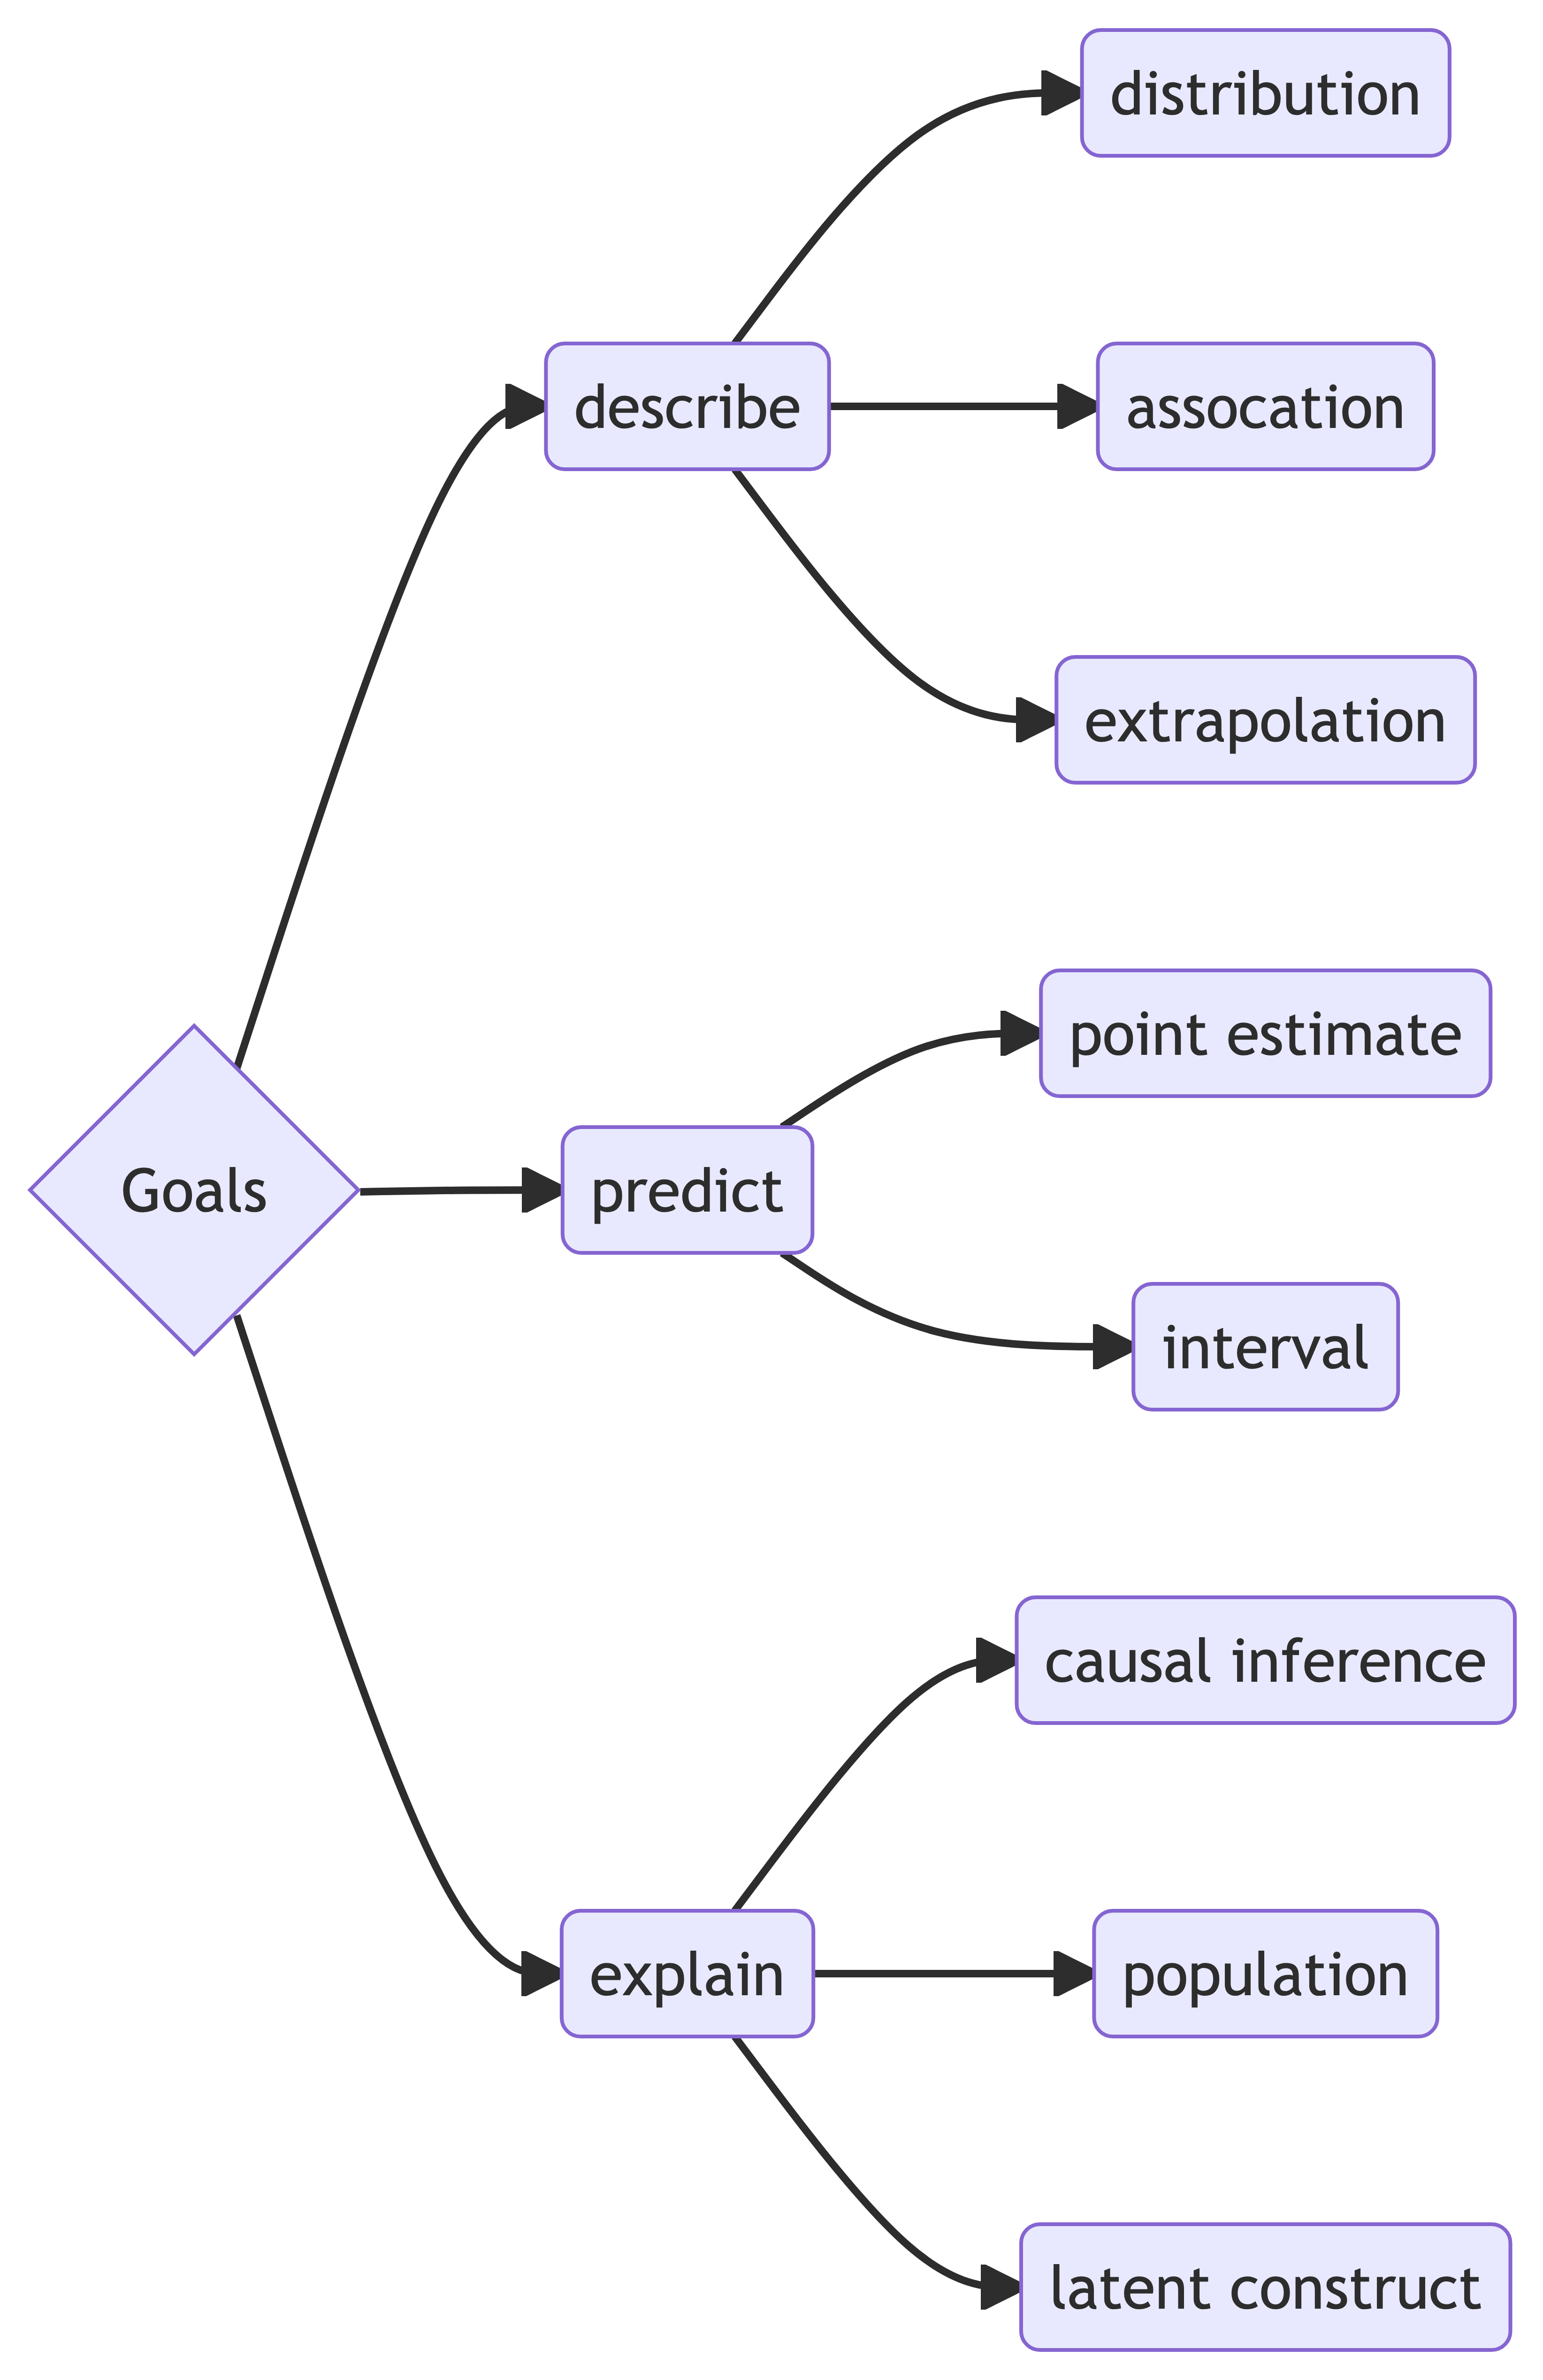
\includegraphics[width=5.5in,height=3.5in]{./goals_files/figure-latex/mermaid-figure-1.png}

}

\end{figure}

}

\caption{\label{fig-goals}A taxonomy of statistical goals}

\end{figure}

\begin{tcolorbox}[enhanced jigsaw, bottomrule=.15mm, toprule=.15mm, coltitle=black, breakable, title=\textcolor{quarto-callout-note-color}{\faInfo}\hspace{0.5em}{Note}, leftrule=.75mm, colback=white, bottomtitle=1mm, toptitle=1mm, left=2mm, opacityback=0, titlerule=0mm, colbacktitle=quarto-callout-note-color!10!white, opacitybacktitle=0.6, colframe=quarto-callout-note-color-frame, rightrule=.15mm, arc=.35mm]
Note that ``goals'' do not exist in the world. We make them up in our
heads. Hence, they have no ontological existence, they are
epistemological beasts. This entails that we are free to devise goals as
we wish, provided we can convince ourselves and other souls of the
utility of our creativity.
\end{tcolorbox}

\hypertarget{further-reading}{%
\section{Further reading}\label{further-reading}}

Hernán, Hsu, and Healy (2019) distinguish:

Hernán et al.~(2019) distinguish:

\begin{itemize}
\item
  \emph{Description}: ``How can women aged 60--80 years with stroke
  history be partitioned in classes defined by their characteristics?''
\item
  \emph{Prediction}: ``What is the probability of having a stroke next
  year for women with certain characteristics?''
\item
  \emph{Causal inference}: ``Will starting a statin reduce, on average,
  the risk of stroke in women with certain characteristics?''
\end{itemize}

Gelman, Hill, and Vehtari (2021), chap.~1.1 proposes three
``challenges'' of statistical inference.

\hypertarget{if-nothing-else-helps}{%
\section{If nothing else helps}\label{if-nothing-else-helps}}

Stay calm and behold the
\href{https://upload.wikimedia.org/wikipedia/commons/thumb/6/69/Spiral_of_black_and_white_squares_10_till_repetition_spiraling_in.gif/600px-Spiral_of_black_and_white_squares_10_till_repetition_spiraling_in.gif?20170912223608}{infinity}.

\bookmarksetup{startatroot}

\hypertarget{basics}{%
\chapter{Basics}\label{basics}}

\hypertarget{ppdac-model-as-a-framework-for-problem-solving}{%
\section{PPDAC Model as a framework for problem
solving}\label{ppdac-model-as-a-framework-for-problem-solving}}

The PPDAC Model is a methodological framework (aka a model) for applying
the scientific method to any analytical or research question, or at
least it is applicable to quite a few (MacKay and Oldford 2000). It is
not meant to be a rigid sequence, but rather a cycle that may turn a
number of rounds like a spiral. Statistician Chris Wild puts the PPDAC
cycle in the following figure, see Figure Figure~\ref{fig-ppdac}.

\begin{figure}

{\centering \includegraphics{https://www.stat.auckland.ac.nz/~wild/StatThink/images/99.Investigative.png}

}

\caption{\label{fig-ppdac}PPDAC cycle. Image source: Chris Wild}

\end{figure}

Wild and Pfannkuch (1999) give a more systematic overview on how a
quantitative research question - applied or basic - can be tackled and
conceived. For example, in their paper the authors enumarate some
dispositions that researcher should embrace in order to fruitfully
engage in empirical research:

\begin{itemize}
\tightlist
\item
  Scepticism
\item
  Imagination
\item
  Curiosity
\item
  Opennness
\item
  A propsenisty to seek deeper menaing
\item
  Being logical
\item
  Engagement
\item
  Perseverance
\end{itemize}

Wild and Pfannkuch (1999) further note that variation is one of the
essential characteristics of data. They discern to types of variation
however, see Figure Figure~\ref{fig-variation}.

\begin{figure}

{\centering \includegraphics{https://www.stat.auckland.ac.nz/~wild/StatThink/images/99.Variation1.png}

}

\caption{\label{fig-variation}Two types of variartion. Image source:
Chris Wild}

\end{figure}

\hypertarget{r-basics}{%
\section{R Basics}\label{r-basics}}

Check out \href{https://moderndive.com/1-getting-started.html}{chapter 1
in ModernDive} for an accessible introduction to getting started with R
and RStudio.

Please also note that R and RStudio should be installed before starting
(this course).

\hypertarget{initial-quiz}{%
\section{Initial quiz}\label{initial-quiz}}

To get an idea whether you have digested some R basics, consider the
following quiz.

\leavevmode\vadjust pre{\hypertarget{exr-q1}{}}%
\begin{exercise}[Define a variable]\label{exr-q1}

Define in R the variable \texttt{age} and assign the value
\texttt{42}.\footnote{\texttt{age\ \textless{}-\ 42}, spaces are
  optional but useful}

\end{exercise}

\leavevmode\vadjust pre{\hypertarget{exr-q2}{}}%
\begin{exercise}[Define a variable as a string]\label{exr-q2}

Define in R the variable \texttt{name} and assign the value
\texttt{me}.\footnote{\texttt{age\ \textless{}-\ "me"}}

\end{exercise}

\leavevmode\vadjust pre{\hypertarget{exr-q3}{}}%
\begin{exercise}[Define a variable by another variable]\label{exr-q3}

Define in R the variable \texttt{name} and assign the \emph{variable}
\texttt{age}.\footnote{\texttt{age\ \textless{}-\ age}}

\end{exercise}

\leavevmode\vadjust pre{\hypertarget{exr-q3a}{}}%
\begin{exercise}[Call a function]\label{exr-q3a}

Ask R what today's \texttt{date()} is, that is, call a
function.\footnote{\texttt{date()}}

\end{exercise}

\leavevmode\vadjust pre{\hypertarget{exr-q4}{}}%
\begin{exercise}[Define a vector]\label{exr-q4}

Define in R a vector \texttt{x} with the values 1,2,3 .\footnote{\texttt{x\ \textless{}-\ c(1,\ 2,\ 3)}}

\end{exercise}

\leavevmode\vadjust pre{\hypertarget{exr-q5}{}}%
\begin{exercise}[Vector wise computation]\label{exr-q5}

Square each value in the vector \texttt{x}.\footnote{\texttt{x\^{}2}}

\end{exercise}

\leavevmode\vadjust pre{\hypertarget{exr-q6}{}}%
\begin{exercise}[Vector wise computation 2]\label{exr-q6}

Square each value in the vector \texttt{x} and sum up the
values.\footnote{\texttt{sum(x\^{}2)}}

\end{exercise}

\leavevmode\vadjust pre{\hypertarget{exr-q7}{}}%
\begin{exercise}[Vector wise computation 3]\label{exr-q7}

Square each value in the vector \texttt{x}, sum up the values, and
divide by 3.\footnote{\texttt{mean(x\^{}2)}}

\end{exercise}

\leavevmode\vadjust pre{\hypertarget{exr-q8}{}}%
\begin{exercise}[Compute the variance]\label{exr-q8}

Compute the variance of \texttt{x} using basic
arithmetic.\footnote{\texttt{sum(x\^{}2)}}\footnote{\begin{Shaded}
\begin{Highlighting}[]
\NormalTok{x }\OtherTok{\textless{}{-}} \FunctionTok{c}\NormalTok{(}\DecValTok{1}\NormalTok{, }\DecValTok{2}\NormalTok{, }\DecValTok{3}\NormalTok{)}

\FunctionTok{sum}\NormalTok{((x }\SpecialCharTok{{-}} \FunctionTok{mean}\NormalTok{(x))}\SpecialCharTok{\^{}}\DecValTok{2}\NormalTok{) }\SpecialCharTok{/}\NormalTok{ (}\FunctionTok{length}\NormalTok{(x)}\SpecialCharTok{{-}}\DecValTok{1}\NormalTok{)}
\end{Highlighting}
\end{Shaded}

\begin{Verbatim}
[1] 1
\end{Verbatim}

\begin{Shaded}
\begin{Highlighting}[]
\CommentTok{\# compare: }
\FunctionTok{var}\NormalTok{(x)  }
\end{Highlighting}
\end{Shaded}

\begin{Verbatim}
[1] 1
\end{Verbatim}
}

\end{exercise}

\leavevmode\vadjust pre{\hypertarget{exr-q9}{}}%
\begin{exercise}[Work with NA]\label{exr-q9}

Define the vector \texttt{y} with the values 1,2,NA. Compute the mean.
Explain the results.\footnote{\texttt{y\ \textless{}-\ c(1,\ 2,\ NA);\ mean(y)}
  NA (not available, ie., missing) is contagious in R: If there's a
  missing element, R will assume that something has gone wrong and will
  raise a red flag, i.e, give you a NA back.}

\end{exercise}

\hypertarget{data-import}{%
\section{Data import}\label{data-import}}

Check out \href{https://moderndive.com/4-tidy.html}{chapter 4 in
ModernDive} on how to import data into RStudio and for some basic
concepts about ``tidy data''.

Spoiler: There's a button in RStudio in the ``Environment'' Pane saying
``Import Dataset''. Just click it, and things should work out.

\hypertarget{sec-blitz-data}{%
\section{Blitz start with data}\label{sec-blitz-data}}

To blitz start with data, type the following in R:

\begin{Shaded}
\begin{Highlighting}[]
\FunctionTok{data}\NormalTok{(mtcars)}
\end{Highlighting}
\end{Shaded}

And the data set \texttt{mtcars} will be available.

To get help for the data set, type \texttt{help(mtcars)}

A bit more advanced, but it's a nice data set, try the Palmer Penguins
data set:

\begin{Shaded}
\begin{Highlighting}[]
\NormalTok{d }\OtherTok{\textless{}{-}} \FunctionTok{read.csv}\NormalTok{(}\StringTok{"https://vincentarelbundock.github.io/Rdatasets/csv/palmerpenguins/penguins.csv"}\NormalTok{)}

\FunctionTok{head}\NormalTok{(d)  }\CommentTok{\# see the first few rows, the "head" of the table}
\end{Highlighting}
\end{Shaded}

\begin{verbatim}
  X species    island bill_length_mm bill_depth_mm flipper_length_mm
1 1  Adelie Torgersen           39.1          18.7               181
2 2  Adelie Torgersen           39.5          17.4               186
3 3  Adelie Torgersen           40.3          18.0               195
4 4  Adelie Torgersen             NA            NA                NA
5 5  Adelie Torgersen           36.7          19.3               193
6 6  Adelie Torgersen           39.3          20.6               190
  body_mass_g    sex year
1        3750   male 2007
2        3800 female 2007
3        3250 female 2007
4          NA   <NA> 2007
5        3450 female 2007
6        3650   male 2007
\end{verbatim}

Here's some
\href{https://vincentarelbundock.github.io/Rdatasets/doc/palmerpenguins/penguins.html}{documentation
(code book)} for this data set.

\hypertarget{more-data-set}{%
\section{More data set}\label{more-data-set}}

Check out
\href{https://data-se.netlify.app/2022/02/23/data-sets-for-for-teaching/}{this
curated list} of data sets useful for learning and practicing your data
skills.

\hypertarget{literature}{%
\section{Literature}\label{literature}}

Ismay and Kim (2020) is a helpful start into the first steps in R.

\bookmarksetup{startatroot}

\hypertarget{exploratory-data-analysis}{%
\chapter{Exploratory Data Analysis}\label{exploratory-data-analysis}}

\includegraphics[width=0.05\textwidth,height=\textheight]{./img/stern.png}

\hypertarget{r-packages-needed-for-this-chapter}{%
\section{R packages needed for this
chapter}\label{r-packages-needed-for-this-chapter}}

\begin{Shaded}
\begin{Highlighting}[]
\FunctionTok{library}\NormalTok{(easystats)}
\FunctionTok{library}\NormalTok{(tidyverse)}
\FunctionTok{library}\NormalTok{(rstanarm)  }\CommentTok{\# optional!}
\end{Highlighting}
\end{Shaded}

\hypertarget{whats-eda}{%
\section{What's EDA?}\label{whats-eda}}

Exploratory Data Analysis (EDA) is a procedure to scrutinize a dataset
at hand in order learn about it. EDA comprises descriptive statistics,
data visualization and data transformation techniques (such as dimension
reduction).

It's not so mathematical deep as modelling, but in practice it's really
important.

There's this famous saying:

\begin{quote}
In Data Science, 80\% of time spent prepare data, 20\% of time spent
complain about the need to prepare data.
\end{quote}

EDA can roughly be said to comprise the following parts:

\begin{itemize}
\tightlist
\item
  Importing (and exporting) data
\item
  Data cleansing (such as deal with missing data etc)
\item
  Data transformation or ``wrangling'' (such as long to wide format)
\item
  Computing desriptive statistics (such as the notorious mean)
\item
  Analyzing distributions (is it normal?)
\item
  Finding patterns in data (aka data mining)
\item
  More complex data transformation techniques (such as factor analysis)
\end{itemize}

\hypertarget{data-journey}{%
\section{Data journey}\label{data-journey}}

Wickham and Grolemund (2016) present a visual sketch of what could be
called the ``data journey'', i.e., the steps we are taking in order to
learn from data, seen from an hands-on angle, see
Figure~\ref{fig-data-journey}.

\begin{figure}

{\centering 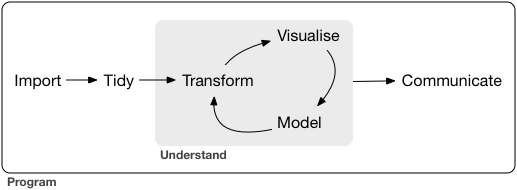
\includegraphics{./img/data-journey.png}

}

\caption{\label{fig-data-journey}The data journey}

\end{figure}

\hypertarget{blitz-data}{%
\section{Blitz data}\label{blitz-data}}

See Section~\ref{sec-blitz-data} for some data sets suitable to get
going.

\hypertarget{data-explorer}{%
\section{Data Explorer}\label{data-explorer}}

There are many systems and approaches to explore data. One particular
interesting system is the R-package \texttt{DataExplorer}.

\begin{figure}

{\centering 
\includegraphics[width=0.2\textwidth,height=\textheight]{./img/dataexplorer-logo.png}

}

\caption{R-package DataExplorer}

\end{figure}

Check it out \href{http://boxuancui.github.io/DataExplorer/}{on its
Githup page}.

\hypertarget{vtree}{%
\section{vtree}\label{vtree}}

A bit similar to \{DataExplorer\}, the
\href{https://nbarrowman.github.io/vtree}{R package \{vtree\}} helps to
explore visually datasets.

\begin{figure}

{\centering 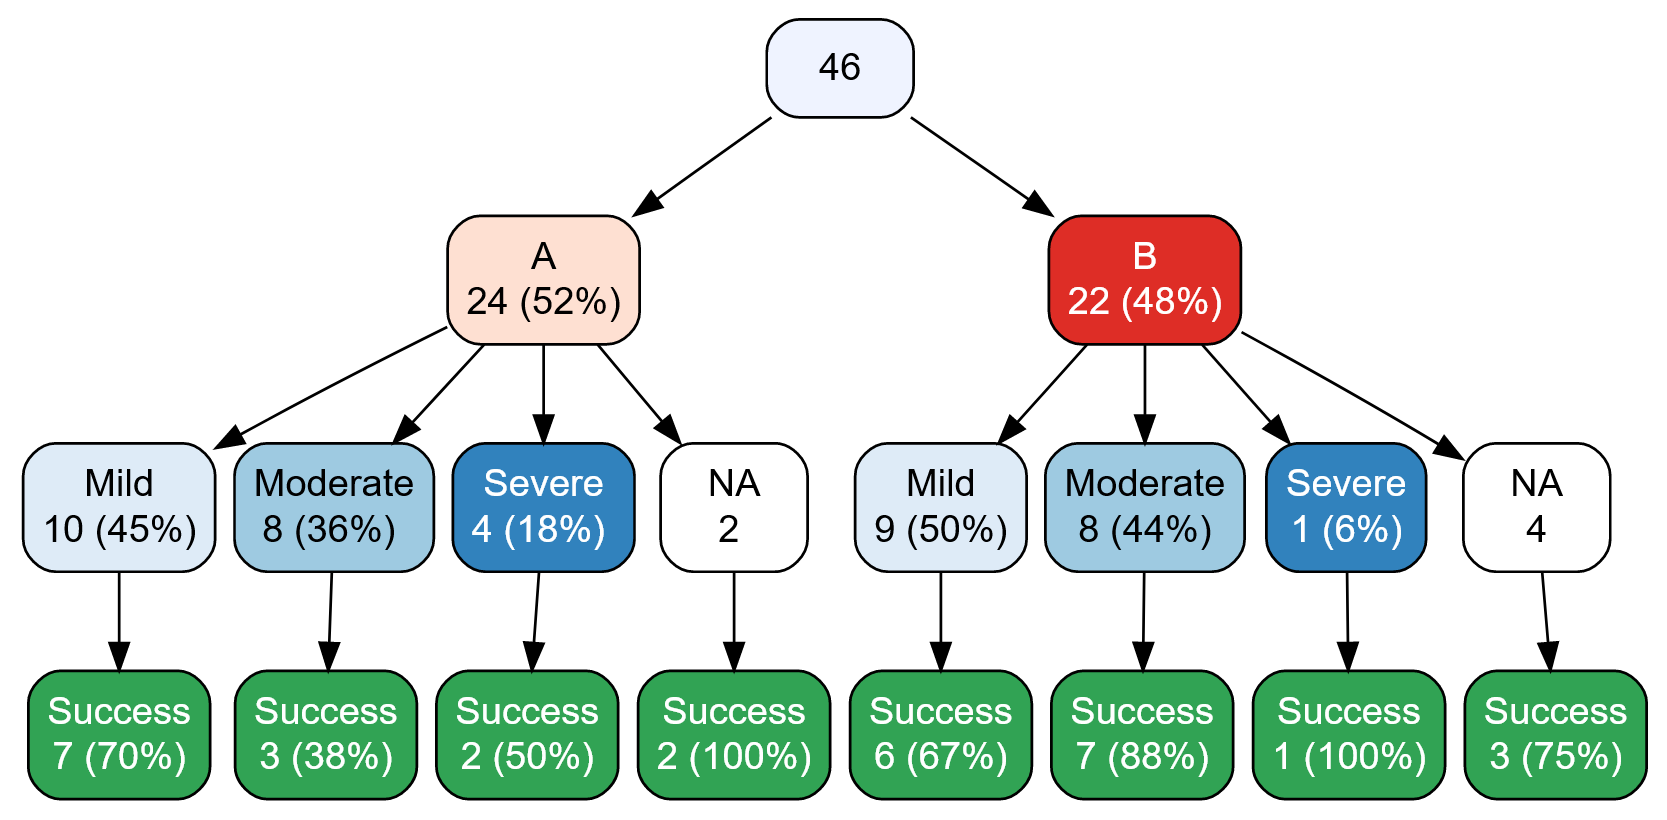
\includegraphics{./img/vtree-vertical.png}

}

\caption{vtree is used to generate variable trees, like the one above.}

\end{figure}

\hypertarget{tidyverse}{%
\section{Tidyverse}\label{tidyverse}}

The Tidyverse is probably the R thing with the most publicity. And it's
great. It's a philosophy baken into an array of R packages. Perhaps
central is the idea that a lot of little lego pieces, if fitting nicely
together, provides a simple yet flexibel and thus powerful machinery.

\hypertarget{janitor}{%
\section{janitor}\label{janitor}}

The R package \{janitor\} provides some nice stuff for data cleansing.
Check out
\href{https://www.exploringdata.org/post/how-to-clean-data-janitor-package/}{this
case study}.

\hypertarget{the-easystats-way}{%
\section{The easystats way}\label{the-easystats-way}}

There are some packages, such as \texttt{\{easystats\}}, which provide
comfortable access to basic statistics:

\begin{Shaded}
\begin{Highlighting}[]
\FunctionTok{library}\NormalTok{(easystats)  }\CommentTok{\# once per session}
\FunctionTok{describe\_distribution}\NormalTok{(mtcars)}
\end{Highlighting}
\end{Shaded}

\begin{verbatim}
Variable |   Mean |     SD |    IQR |           Range | Skewness | Kurtosis |  n | n_Missing
--------------------------------------------------------------------------------------------
mpg      |  20.09 |   6.03 |   7.53 |  [10.40, 33.90] |     0.67 |    -0.02 | 32 |         0
cyl      |   6.19 |   1.79 |   4.00 |    [4.00, 8.00] |    -0.19 |    -1.76 | 32 |         0
disp     | 230.72 | 123.94 | 221.53 | [71.10, 472.00] |     0.42 |    -1.07 | 32 |         0
hp       | 146.69 |  68.56 |  84.50 | [52.00, 335.00] |     0.80 |     0.28 | 32 |         0
drat     |   3.60 |   0.53 |   0.84 |    [2.76, 4.93] |     0.29 |    -0.45 | 32 |         0
wt       |   3.22 |   0.98 |   1.19 |    [1.51, 5.42] |     0.47 |     0.42 | 32 |         0
qsec     |  17.85 |   1.79 |   2.02 |  [14.50, 22.90] |     0.41 |     0.86 | 32 |         0
vs       |   0.44 |   0.50 |   1.00 |    [0.00, 1.00] |     0.26 |    -2.06 | 32 |         0
am       |   0.41 |   0.50 |   1.00 |    [0.00, 1.00] |     0.40 |    -1.97 | 32 |         0
gear     |   3.69 |   0.74 |   1.00 |    [3.00, 5.00] |     0.58 |    -0.90 | 32 |         0
carb     |   2.81 |   1.62 |   2.00 |    [1.00, 8.00] |     1.16 |     2.02 | 32 |         0
\end{verbatim}

\texttt{describe\_distribution} provides us with an overview on typical
descriptive summaries.

For nominal variables, consider \texttt{data\_tabulate}:

\begin{Shaded}
\begin{Highlighting}[]
\FunctionTok{data\_tabulate}\NormalTok{(mtcars, }\AttributeTok{select =} \FunctionTok{c}\NormalTok{(}\StringTok{"am"}\NormalTok{, }\StringTok{"vs"}\NormalTok{))}
\end{Highlighting}
\end{Shaded}

\begin{verbatim}
am (am) <numeric>
# total N=32 valid N=32

Value |  N | Raw % | Valid % | Cumulative %
------+----+-------+---------+-------------
0     | 19 | 59.38 |   59.38 |        59.38
1     | 13 | 40.62 |   40.62 |       100.00
<NA>  |  0 |  0.00 |    <NA> |         <NA>

vs (vs) <numeric>
# total N=32 valid N=32

Value |  N | Raw % | Valid % | Cumulative %
------+----+-------+---------+-------------
0     | 18 | 56.25 |   56.25 |        56.25
1     | 14 | 43.75 |   43.75 |       100.00
<NA>  |  0 |  0.00 |    <NA> |         <NA>
\end{verbatim}

We can also get \emph{grouped} tabulations, which amounts to something
similar to a
\href{https://en.wikipedia.org/wiki/Contingency_table}{contingency
table}:

\begin{Shaded}
\begin{Highlighting}[]
\NormalTok{mtcars }\SpecialCharTok{\%\textgreater{}\%} 
  \FunctionTok{group\_by}\NormalTok{(am) }\SpecialCharTok{\%\textgreater{}\%} 
  \FunctionTok{data\_tabulate}\NormalTok{(}\AttributeTok{select =} \StringTok{"vs"}\NormalTok{, }\AttributeTok{collapse =} \ConstantTok{TRUE}\NormalTok{)}
\end{Highlighting}
\end{Shaded}

\begin{verbatim}
# Frequency Table

Variable |  Group | Value |  N | Raw % | Valid % | Cumulative %
---------+--------+-------+----+-------+---------+-------------
vs       | am (0) |     0 | 12 | 63.16 |   63.16 |        63.16
         |        |     1 |  7 | 36.84 |   36.84 |       100.00
         |        |  <NA> |  0 |  0.00 |    <NA> |         <NA>
---------+--------+-------+----+-------+---------+-------------
vs       | am (1) |     0 |  6 | 46.15 |   46.15 |        46.15
         |        |     1 |  7 | 53.85 |   53.85 |       100.00
         |        |  <NA> |  0 |  0.00 |    <NA> |         <NA>
---------------------------------------------------------------
\end{verbatim}

Checkout the function reference of your favorite package in order to
learn what's on the shelf. For example,
\href{https://easystats.github.io/datawizard/reference/index.html}{here's
the function reference site} of \texttt{datawizard}, one of the packages
in the \texttt{easystats} ecosystem.

\hypertarget{case-study-2}{%
\section{Case Study}\label{case-study-2}}

\begin{figure}

{\centering 
\includegraphics[width=0.2\textwidth,height=\textheight]{./img/palmerpenguins-logo.png}

}

\caption{R package/dataset palmerpenguins}

\end{figure}

Explore the \texttt{palmerpenguins} dataset, it's a famous dataset made
for learning data analysis.

There's a great
\href{https://allisonhorst.shinyapps.io/dplyr-learnr/\#section-welcome}{interactive
course on EDA based on the penguins}. Have a look, it's great!

\href{https://media.giphy.com/media/3og0IO5z8Rd30ktV6g/giphy.gif}{Go
penguins! Allez!}

\hypertarget{cheatsheets}{%
\section{Cheatsheets}\label{cheatsheets}}

There are a number of nice cheat sheets
\href{https://www.rstudio.com/resources/cheatsheets/}{available on an
array of topics related to EDA}, made available by the folks at RStudio.

Consider this collection:

\begin{itemize}
\item
  \href{https://raw.githubusercontent.com/rstudio/cheatsheets/main/pngs/data-transformation.png}{\{dplyr\}:
  data wrangling}
\item
  \href{https://raw.githubusercontent.com/rstudio/cheatsheets/main/pngs/tidyr.png}{\{tidyr\}:
  data preparation}
\item
  \href{https://raw.githubusercontent.com/rstudio/cheatsheets/main/pngs/data-visualization.png}{\{ggplot\}:
  data visualization}
\item
  \href{https://raw.githubusercontent.com/rstudio/cheatsheets/main/pngs/gtsummary.png}{\{gtsummary\}:
  publication ready tables}
\end{itemize}

So much great stuff! A bit too much to digest in one go, but definitely
worthwhile if you plan to dig deeper in data analysis.

\hypertarget{literature-1}{%
\section{Literature}\label{literature-1}}

Wickham and Grolemund (2016) is an highly recommendable resource in
order to get a thorough understanding of data analysis using R. Note
that this source is focusing on the ``how to'', not so much to
theoretical foundations. Ismay and Kim (2020) is a gently introduction
into many steps on the data journey, including EDA.

\bookmarksetup{startatroot}

\hypertarget{inference}{%
\chapter{Inference}\label{inference}}

\includegraphics[width=0.05\textwidth,height=\textheight]{./img/stern.png}

\hypertarget{what-is-it}{%
\section{What is it?}\label{what-is-it}}

Statistical inference, according to Gelman, Hill, and Vehtari (2021),
chap.~1.1, faces the challenge of \emph{generalizing} from the
particular to the general.

In more details, this amounts to generalizing from \ldots{}

\begin{enumerate}
\def\labelenumi{\arabic{enumi}.}
\tightlist
\item
  a sample to a population
\item
  a treatment to a control group (i.e., causal inference)
\item
  observed measurement to the underlying (``latent'') construct of
  interest
\end{enumerate}

\begin{tcolorbox}[enhanced jigsaw, bottomrule=.15mm, toprule=.15mm, coltitle=black, breakable, title=\textcolor{quarto-callout-important-color}{\faExclamation}\hspace{0.5em}{Important}, leftrule=.75mm, colback=white, bottomtitle=1mm, toptitle=1mm, left=2mm, opacityback=0, titlerule=0mm, colbacktitle=quarto-callout-important-color!10!white, opacitybacktitle=0.6, colframe=quarto-callout-important-color-frame, rightrule=.15mm, arc=.35mm]
Statistical inference is concerned with making general claims from
particular data using mathematical tools.
\end{tcolorbox}

\hypertarget{population-and-sample}{%
\section{Population and sample}\label{population-and-sample}}

We want to have an estimate of some population value, for example the
proportion of \texttt{A}.

However, all we have is a subset, a sample of the populuation. Hence, we
need to \emph{infer} from the sample to the popluation. We do so by
generalizing from the sample to the population, see Figure
Figure~\ref{fig-pop-sample}.

\begin{figure}

\begin{minipage}[t]{0.50\linewidth}

{\centering 

\raisebox{-\height}{

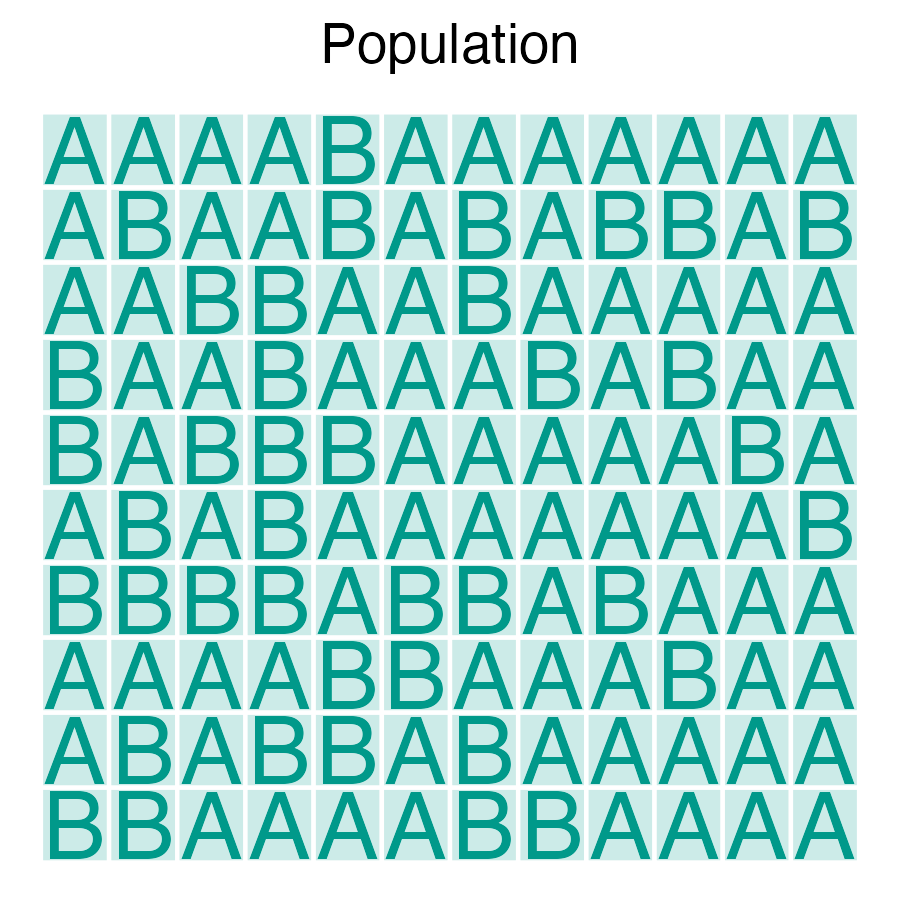
\includegraphics{./img/pvoll.png}

}

}

\subcaption{\label{fig-pop}Population}
\end{minipage}%
%
\begin{minipage}[t]{0.50\linewidth}

{\centering 

\raisebox{-\height}{

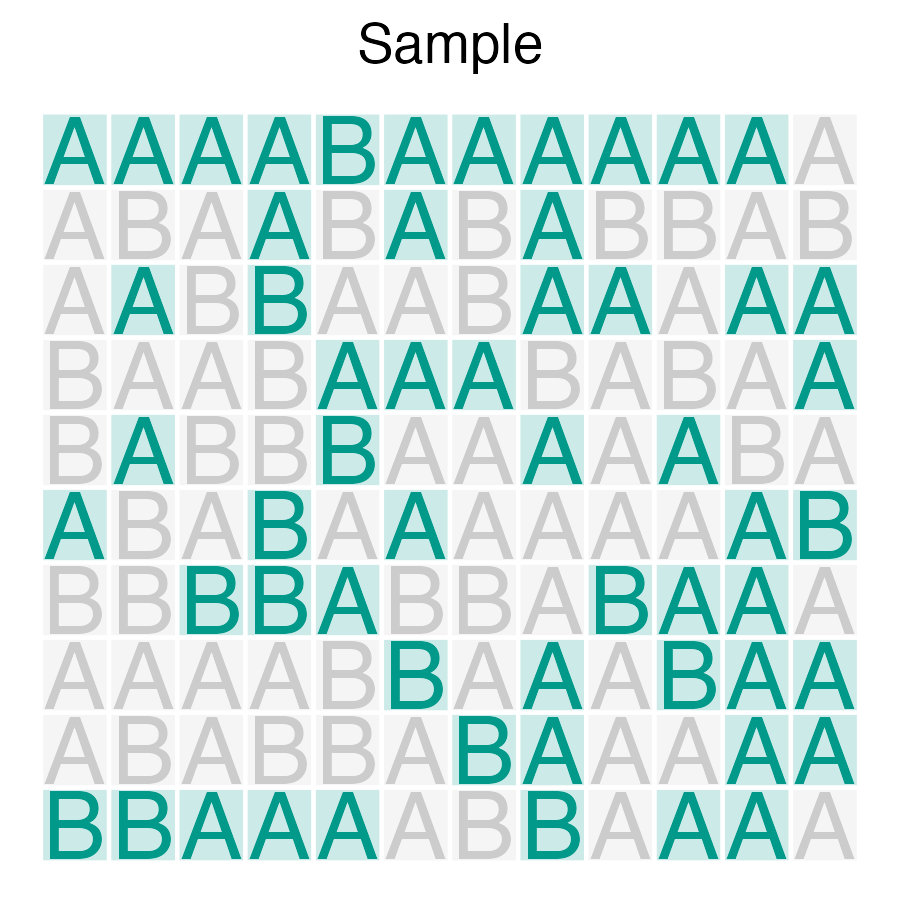
\includegraphics{./img/psti.png}

}

}

\subcaption{\label{fig-sample}Sample}
\end{minipage}%

\caption{\label{fig-pop-sample}Population vs.~sample (Image credit:
Karsten Luebke)}

\end{figure}

\hypertarget{whats-not-inference}{%
\section{What's not inference?}\label{whats-not-inference}}

Consider fig. Figure~\ref{fig-desk-inf} which epitomizes the difference
between \emph{descriptive} and \emph{inferential} statistics.

\begin{figure}

{\centering 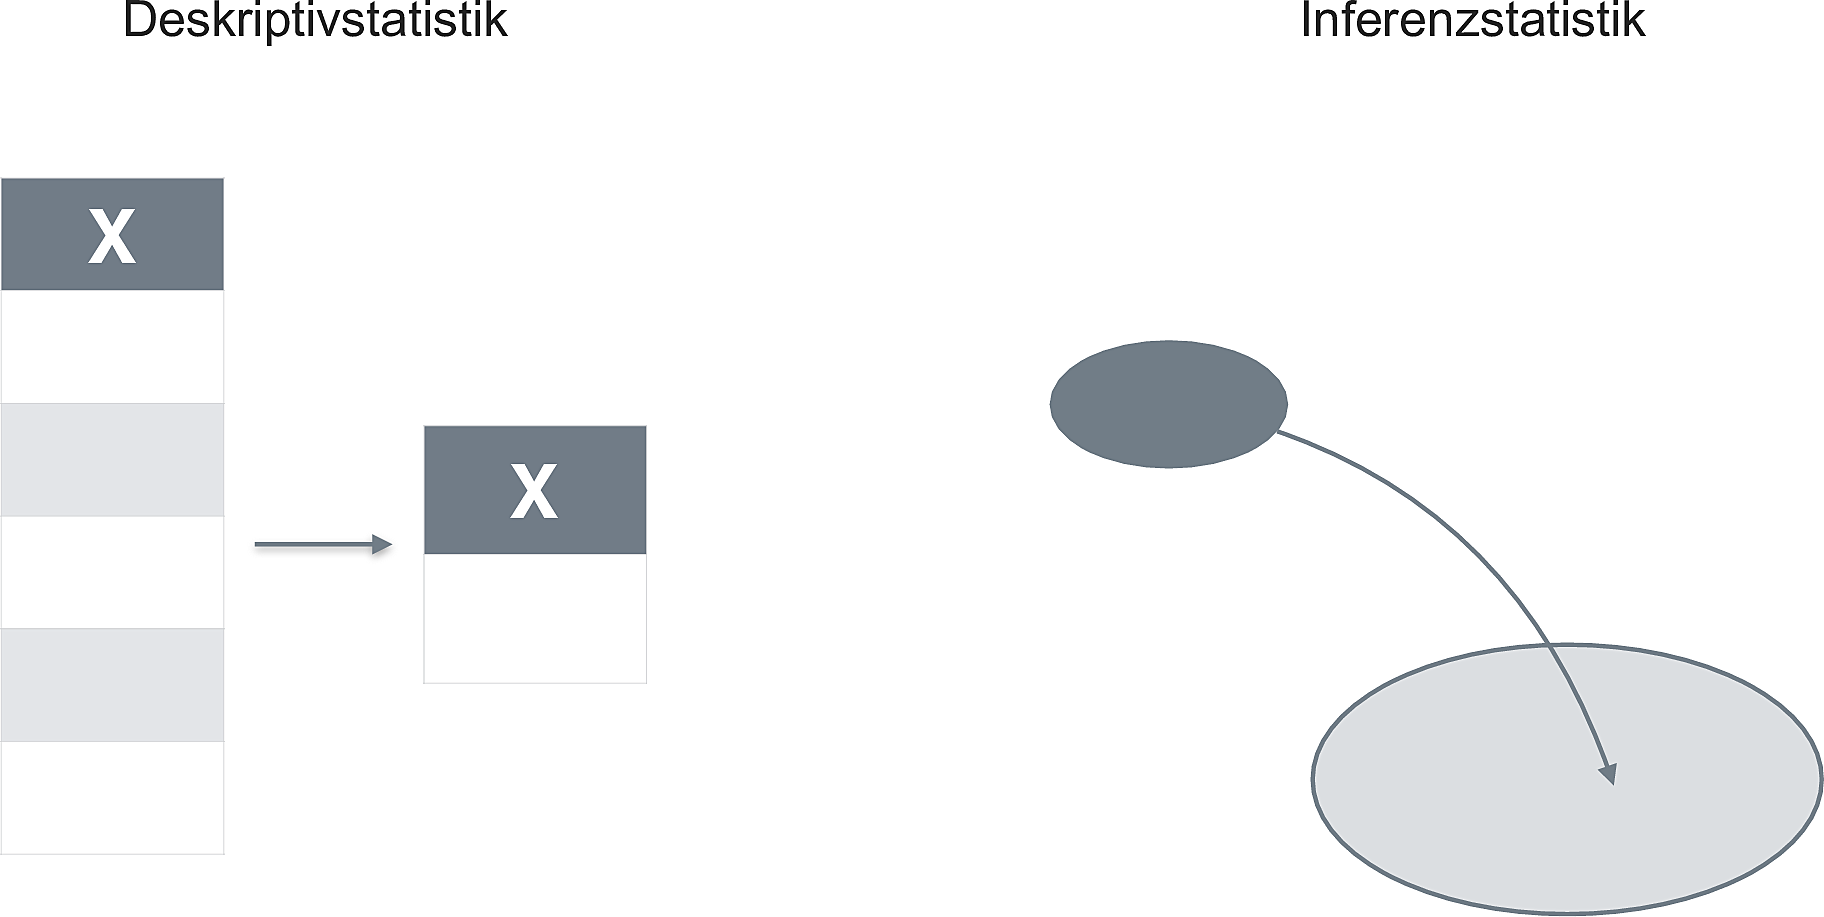
\includegraphics[width=0.5\textwidth,height=\textheight]{./img/desk_vs_inf-crop.png}

}

\caption{\label{fig-desk-inf}The difference between description and
inference}

\end{figure}

\hypertarget{when-size-helps}{%
\section{When size helps}\label{when-size-helps}}

Larger samples allow for more precise estimations (ceteris paribus).

\hypertarget{what-flavors-are-available}{%
\section{What flavors are available?}\label{what-flavors-are-available}}

Typically, when one hears ``inference'' one thinks of p-values and null
hypothesis testing. Those procedures are examples of the school of
\emph{Frequentist statistics}.

However, there's a second flavor of statistics to be mentioned here:
\emph{Bayesian statistics}.

\hypertarget{frequentist-inference}{%
\subsection{Frequentist inference}\label{frequentist-inference}}

Frequentism is \emph{not} concerned about the probability of your
research hypothesis.

Frequentism is all about controlling the \emph{long-term error}. For
illustration, suppose you are the CEO of a factory producing screws, and
many of them. As the boss, you are not so much interested if a
particular scree is in order (or faulty). Rather you are interested that
the overall, long-term error rate of your production is low. One may add
that your goal might not the minimize the long-term error, b ut to
control it to a certain level - it may be to expensive to produce super
high quality screws. Some decent, but cheap screws, might be more
profitable.

\hypertarget{bayes-inference}{%
\subsection{Bayes inference}\label{bayes-inference}}

Bayes inference is concerned about the probability of your research
hypothesis.

It simply redistributes your beliefs based on new data (evidence) you
observe, see Figure \textbf{?@fig-belief-update}:

In more detail, the posterior belief is formalized as the posterior
probability. The Likelihood is the probability of the data given some
hypothesis. The normalizing constant serves to give us a number between
zero and one.

\[\overbrace{\Pr(\color{blue}{H}|\color{green}{D})}^\text{posterior probability} = \overbrace{Pr(\color{blue}{H})}^\text{prior} \frac{\overbrace{Pr(\color{green}{D}|\color{blue}{H})}^\text{likelihood}}{\underbrace{Pr(\color{green}{D})}_{\text{normalizing constant}}}\]

In practice, the posterior probability of your hypothesis is, the
average of your prior and the Likelihood of your data.

\begin{figure}

{\centering 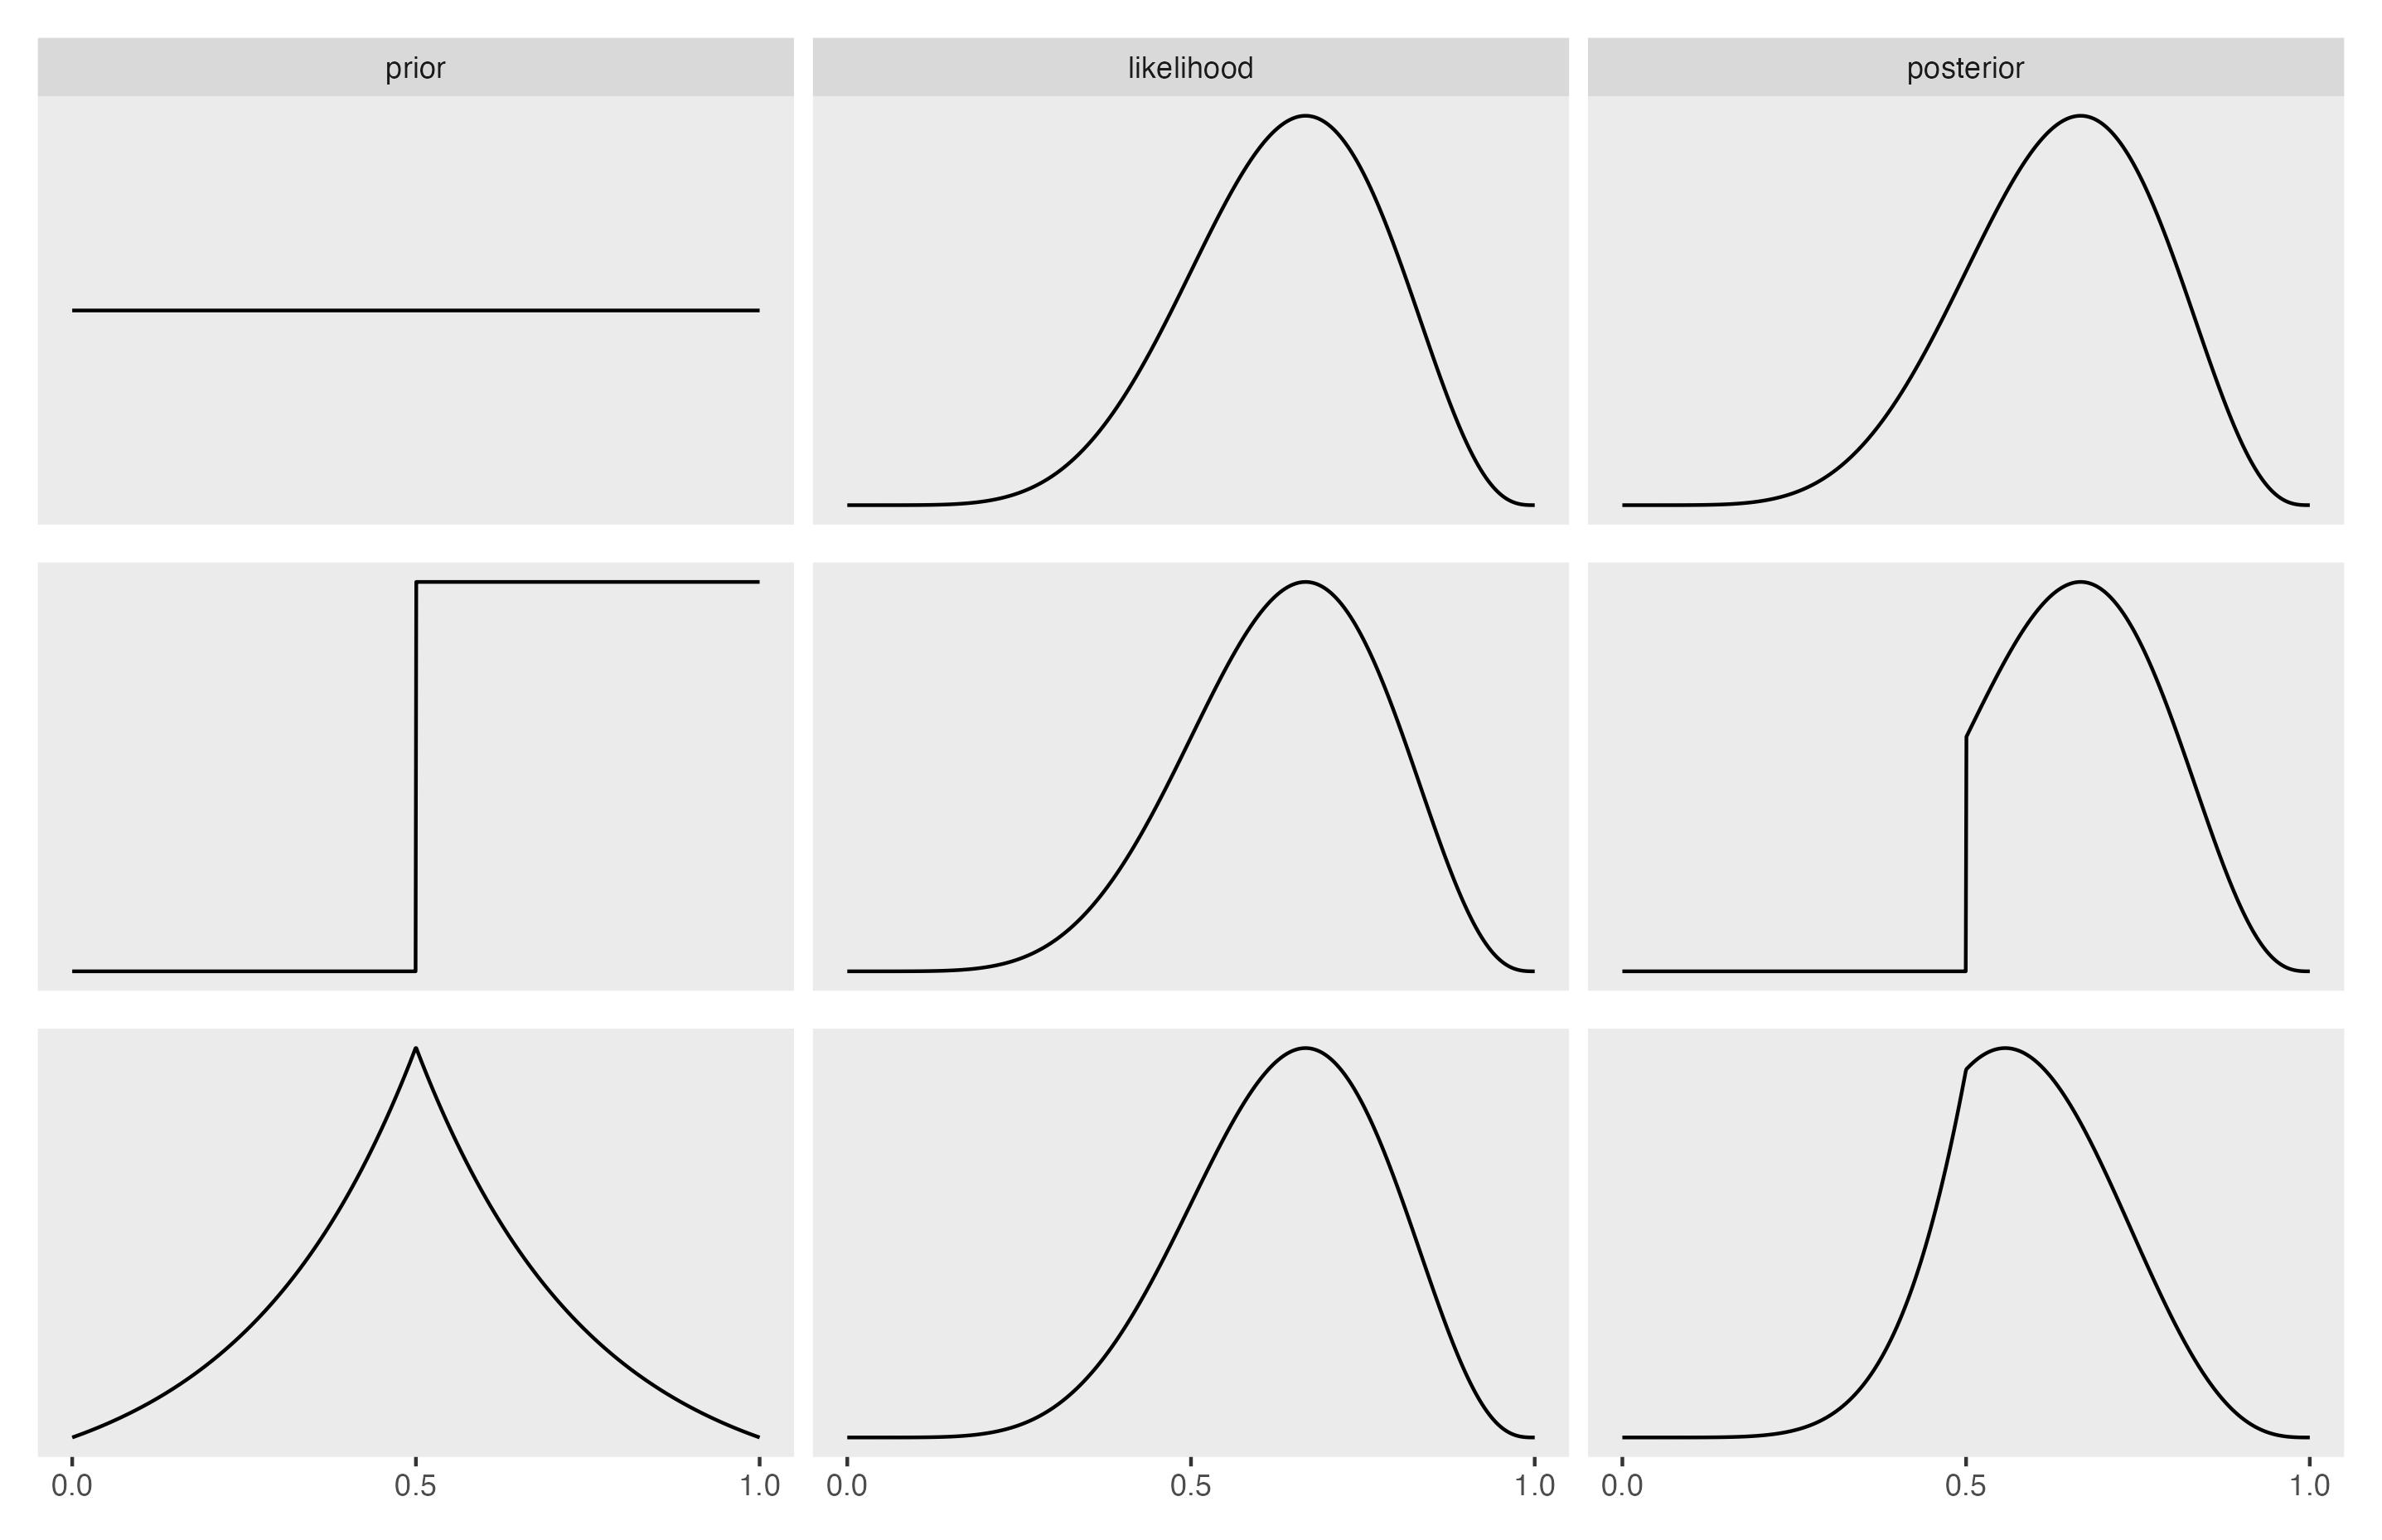
\includegraphics[width=0.7\textwidth,height=\textheight]{./img/prior-l-post.png}

}

\caption{Prior-Likelihood-Posterior}

\end{figure}

Can you see that the posterior is some average of prior and likelihood?

Check out this \href{https://youtu.be/HZGCoVF3YvM}{great video on Bayes
Theorem by 3b1b}.

\hypertarget{but-which-one-should-i-consume}{%
\section{But which one should I
consume?}\label{but-which-one-should-i-consume}}

PRO Frequentist:

\begin{itemize}
\tightlist
\item
  Your supervisor and reviewers will be more familiar with it
\item
  The technical overhead is simpler compared to Bayes
\end{itemize}

PRO Bayes:

\begin{itemize}
\tightlist
\item
  You'll probably want to have a posterior probability of your
  hypothesis
\item
  You may appear as a cool kid and an early adoptor of emering
  statistical methods
\end{itemize}

\begin{tcolorbox}[enhanced jigsaw, bottomrule=.15mm, toprule=.15mm, coltitle=black, breakable, title=\textcolor{quarto-callout-tip-color}{\faLightbulb}\hspace{0.5em}{Tip}, leftrule=.75mm, colback=white, bottomtitle=1mm, toptitle=1mm, left=2mm, opacityback=0, titlerule=0mm, colbacktitle=quarto-callout-tip-color!10!white, opacitybacktitle=0.6, colframe=quarto-callout-tip-color-frame, rightrule=.15mm, arc=.35mm]
You'll learn that the technical setup used for doing Bayes statistics is
quite similar to doing frequentist statistics. Stay tuned.
\end{tcolorbox}

\hypertarget{comment-from-xkcd}{%
\section{Comment from xkcd}\label{comment-from-xkcd}}

\begin{figure}

{\centering 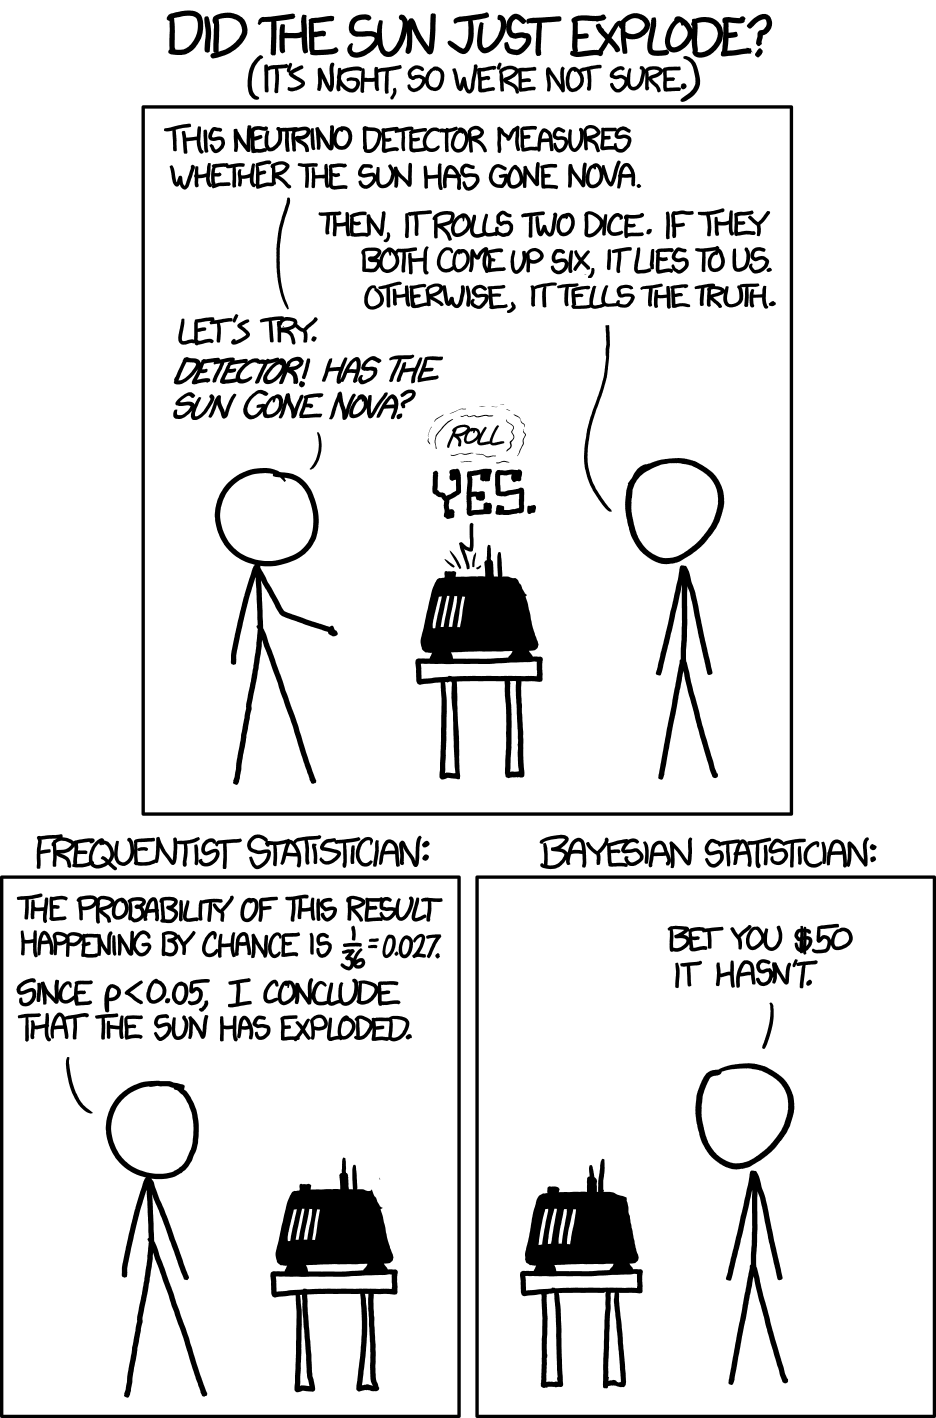
\includegraphics[width=0.5\textwidth,height=\textheight]{./img/frequentists_vs_bayesians_2x.png}

}

\end{figure}

\href{https://xkcd.com/1132/}{Quelle}

\hypertarget{p-value}{%
\section{p-value}\label{p-value}}

The p-value has been used as the pivotal criterion to decide about
whether or not a research hypothesis were to be ``accepted'' (a term
forbidden in frequentist and Popperian langauge) or to be rejected.
However, more recently, it is advised to use the p-value only as
\emph{one} indicator among multiple; see Wasserstein and Lazar (2016)
and Wasserstein, Schirm, and Lazar (2019).

\begin{tcolorbox}[enhanced jigsaw, bottomrule=.15mm, toprule=.15mm, coltitle=black, breakable, title=\textcolor{quarto-callout-important-color}{\faExclamation}\hspace{0.5em}{Important}, leftrule=.75mm, colback=white, bottomtitle=1mm, toptitle=1mm, left=2mm, opacityback=0, titlerule=0mm, colbacktitle=quarto-callout-important-color!10!white, opacitybacktitle=0.6, colframe=quarto-callout-important-color-frame, rightrule=.15mm, arc=.35mm]
The p-value is defined as the probability of obtaining the observed data
(or more extreme) under the assumption of no effect.
\end{tcolorbox}

Figure Figure~\ref{fig-pvalue} visualizes the p-value.

\begin{figure}

{\centering 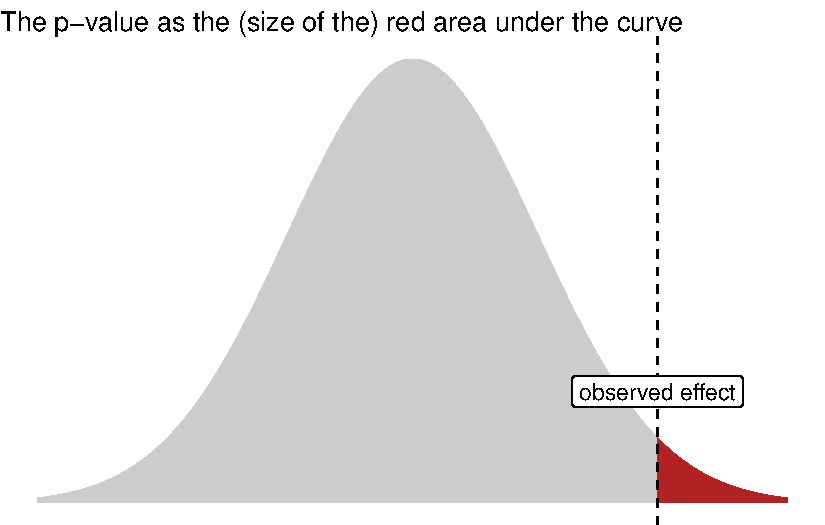
\includegraphics[width=0.5\textwidth,height=\textheight]{./inference_files/figure-pdf/fig-pvalue-1.pdf}

}

\caption{\label{fig-pvalue}Visualization of the p-value}

\end{figure}

\hypertarget{some-confusion-remains-about-the-p-value}{%
\section{Some confusion remains about the
p-value}\label{some-confusion-remains-about-the-p-value}}

\begin{figure}

{\centering 
\includegraphics[width=0.25\textwidth,height=\textheight]{./img/6m29tz.jpeg}

}

\caption{Source: from ImgFlip Meme Generator}

\end{figure}

Goodman (2008) provides an entertaining overview on typical
misconceptions of the p-value
\href{https://www.ohri.ca//newsroom/seminars/SeminarUploads/1829/Suggested\%20Reading\%20-\%20Nov\%203,\%202014.pdf}{full
text}.

\bookmarksetup{startatroot}

\hypertarget{modelling-and-regression}{%
\chapter{Modelling and regression}\label{modelling-and-regression}}

\includegraphics[width=0.05\textwidth,height=\textheight]{./img/stern.png}

\hypertarget{r-packages-needed-for-this-chapter-1}{%
\section{R packages needed for this
chapter}\label{r-packages-needed-for-this-chapter-1}}

\begin{Shaded}
\begin{Highlighting}[]
\FunctionTok{library}\NormalTok{(easystats)}
\FunctionTok{library}\NormalTok{(tidyverse)}
\FunctionTok{library}\NormalTok{(rstanarm)  }\CommentTok{\# optional!}
\end{Highlighting}
\end{Shaded}

\hypertarget{whats-modelling}{%
\section{What's modelling?}\label{whats-modelling}}

\href{https://statsthinking21.github.io/statsthinking21-core-site/fitting-models.html\#what-is-a-model}{Read
this great introduction by modelling by Russel Poldrack}. Actually, the
whole book is nice Poldrack (2022).

An epitome of modelling is this, let's call it the fundamental modelling
equation, a bit grandiose but at the point, see
Equation~\ref{eq-modelling}.

The data can be separated in the model's prediction and the rest (the
``error''), i.e., what's unaccounted for by the model.

\begin{equation}\protect\hypertarget{eq-modelling}{}{
\text{data} = \text{model} + \text{error}
}\label{eq-modelling}\end{equation}

A more visual account of our basic modelling equation is depicted in
\textbf{?@fig-model1}.

\hypertarget{regression-as-the-umbrella-tool-for-modelling}{%
\section{Regression as the umbrella tool for
modelling}\label{regression-as-the-umbrella-tool-for-modelling}}


\includegraphics[width=0.5\textwidth,height=\textheight]{./img/one-regression-to-rule-them-all.jpeg}
\href{www.imgflip.com}{Source: Image Flip}

Alternatively, venture into the forest of statistical tests as
\href{https://web.archive.org/web/20091029162244/http://www.wiwi.uni-muenster.de/ioeb/en/organisation/pfaff/stat_overview_table.html}{outlined
e.g.~here, at Uni Muenster}.

You may want to ponder on this image of a decision tree of which test to
choose, see Figure Figure~\ref{fig-choose-test}.

\begin{figure}

{\centering 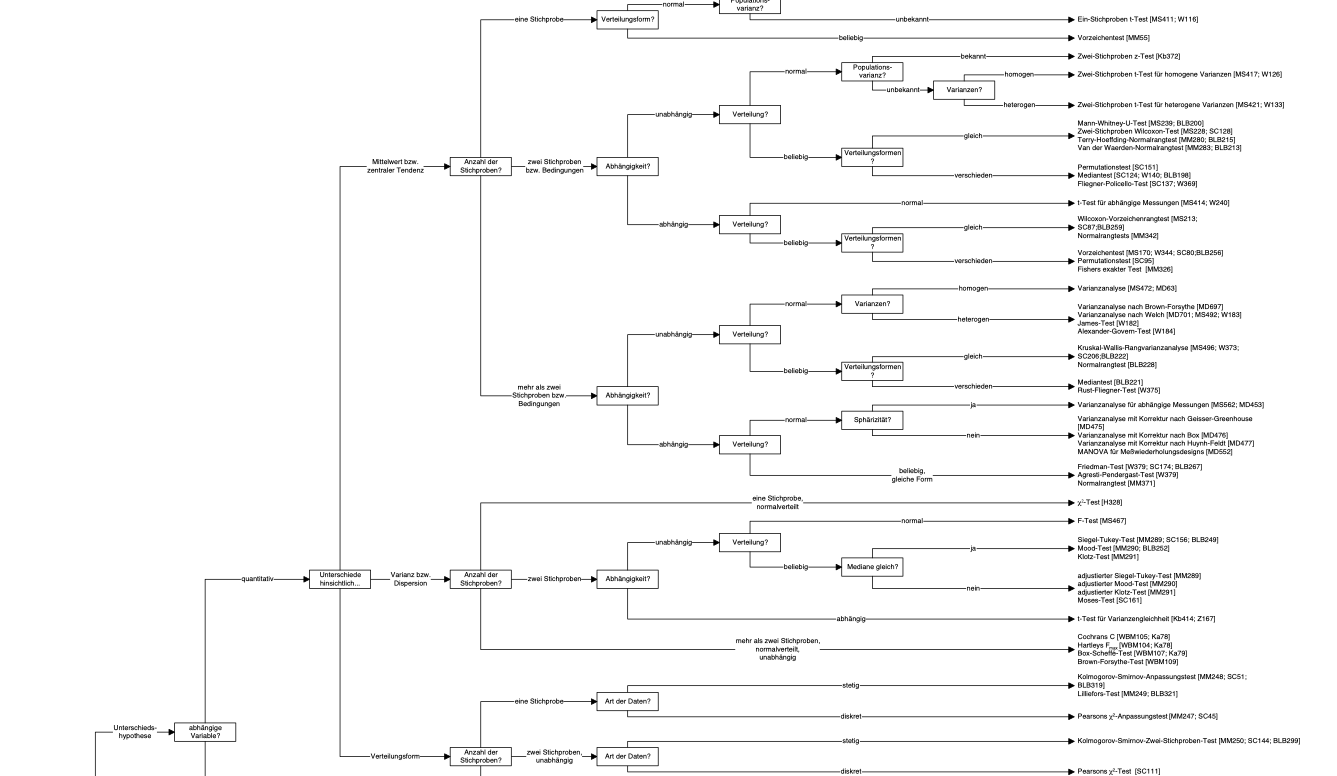
\includegraphics{./img/choose-test.png}

}

\caption{\label{fig-choose-test}Choose your test carefully}

\end{figure}

\hypertarget{common-statistical-tests-are-linear-models}{%
\subsection{Common statistical tests are linear
models}\label{common-statistical-tests-are-linear-models}}

As Jonas Kristoffer Lindeløv tells us, we can formulate most statistical
tests as a linear model, ie., a regression.

\begin{figure}

{\centering 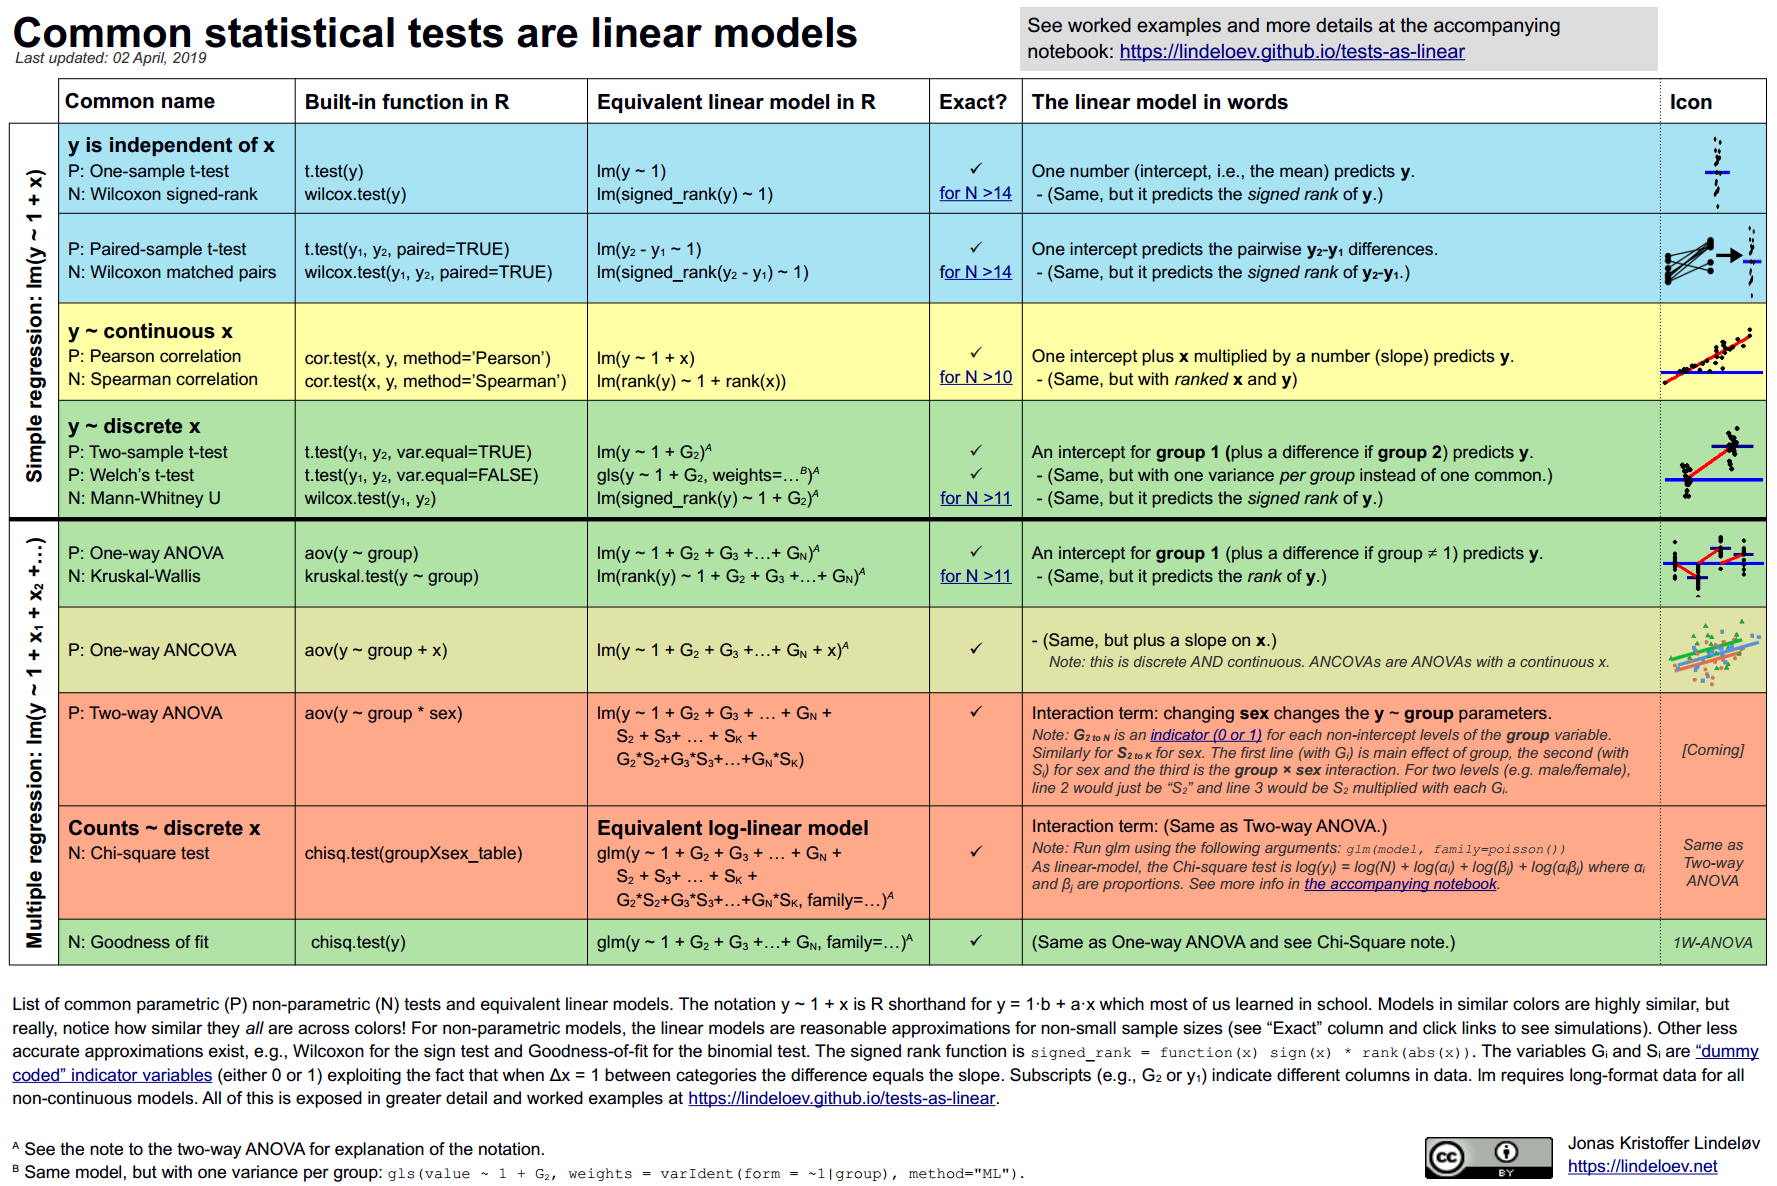
\includegraphics[width=0.75\textwidth,height=\textheight]{./img/linear_tests_cheat_sheet.png}

}

\caption{Common statistical tests as linear models}

\end{figure}

\hypertarget{how-to-find-the-regression-line}{%
\subsection{How to find the regression
line}\label{how-to-find-the-regression-line}}

In the simplest case, regression analyses can be interpreted
geometrically as a line in a 2D coordinate system, see Figure
Figure~\ref{fig-regr1}.

\begin{figure}

{\centering 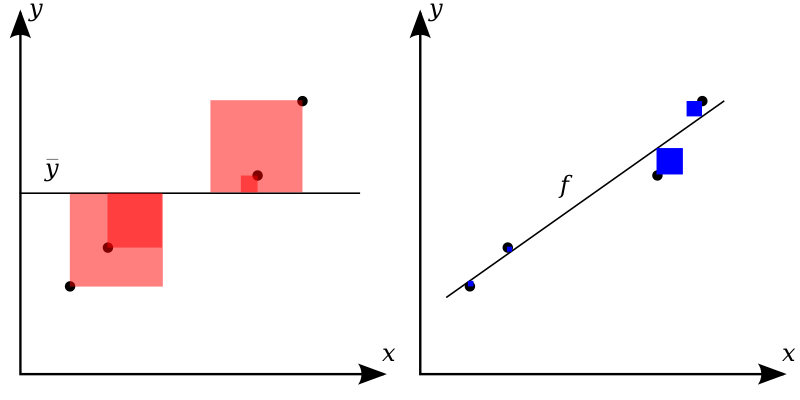
\includegraphics{./img/800px-Coefficient_of_Determination.svg.png}

}

\caption{\label{fig-regr1}Least Square Regression}

\end{figure}

\href{https://commons.wikimedia.org/wiki/File:Coefficient_of_Determination.svg}{Source:
Orzetoo, CC-SA, Wikimedia}

Put simple, we are looking for the line which is in the ``middle of the
points''. More precisely, we place the line such that the squared
distances from the line to the points is minimal, see Figre
Figure~\ref{fig-regr1}.

Consider Figure Figure~\ref{fig-regr2}, from
\href{https://bookdown.org/roback/bookdown-BeyondMLR/ch-MLRreview.html\#assumptions-for-linear-least-squares-regression}{this
source} by Roback and Legler (2021). It visualizes not only the
notorious regression line, but also sheds light on regression
assumptions, particularly on the error distribution.

\begin{figure}

{\centering 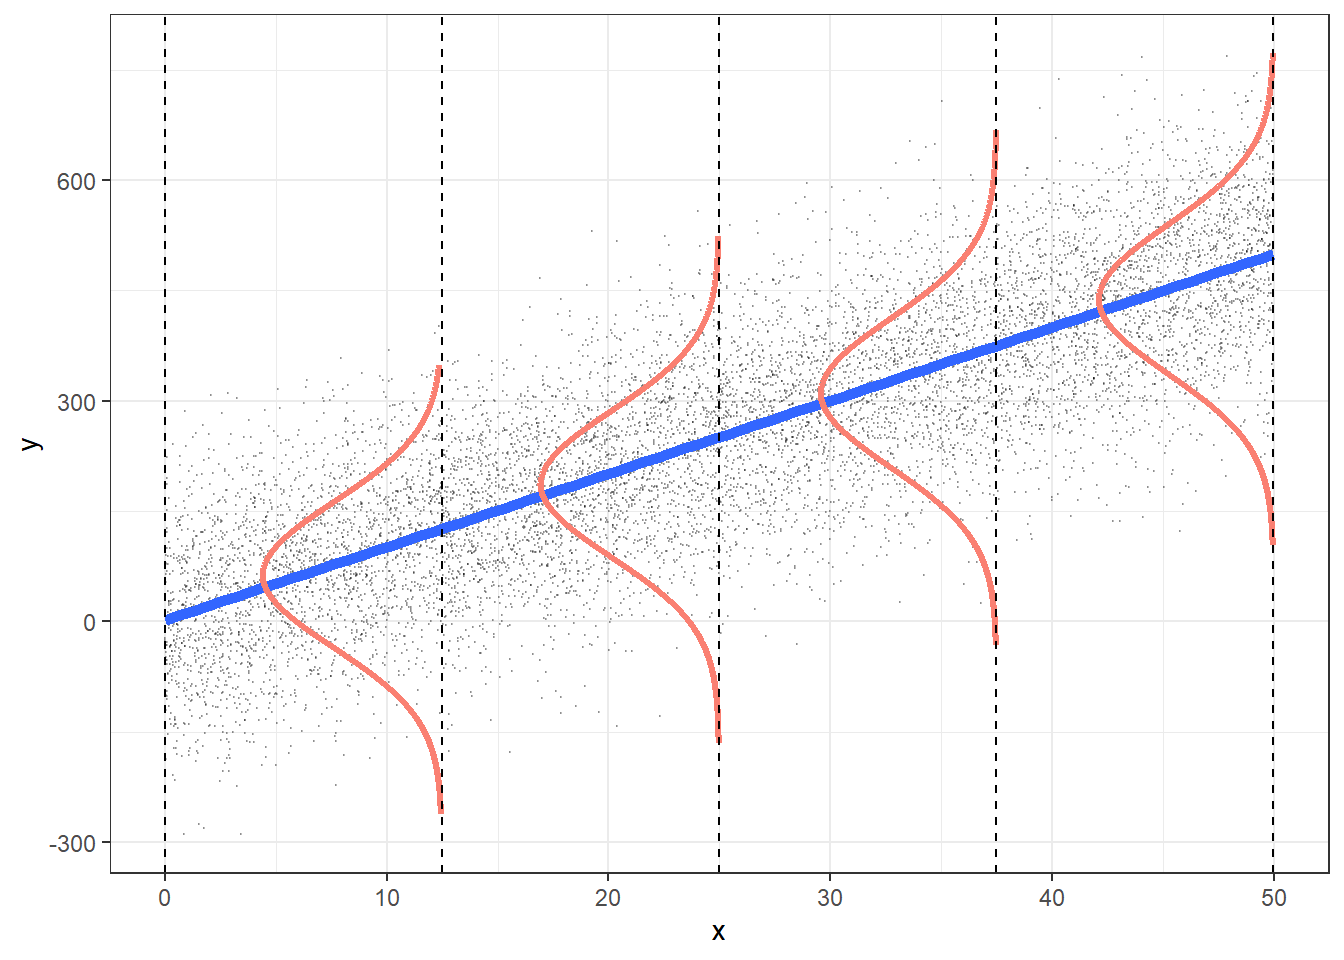
\includegraphics{./img/OLSassumptions-1.png}

}

\caption{\label{fig-regr2}Regression and some of its assumptions}

\end{figure}

\hypertarget{the-linear-model}{%
\subsection{The linear model}\label{the-linear-model}}

Here's the canonical form of the linear model.

Consider a model with \(k\) predictors:

\[y = \beta_0 + \beta_1 x_1 + \ldots + \beta_k x_k + \epsilon\]

\hypertarget{algebraic-derivation}{%
\subsection{Algebraic derivation}\label{algebraic-derivation}}

For the mathematical inclined, check out
\href{https://data-se.netlify.app/2022/05/23/ableitung-der-koeffizienten-der-einfachen-regression/}{this
derivation} of the simple case regression model. Note that the article
is written in German, but your browser can effortlessly translate into
English. Here's a
\href{https://math.stackexchange.com/questions/716826/derivation-of-simple-linear-regression-parameters}{similar
English article from StackExchange}.

\hypertarget{in-all-its-glory}{%
\section{In all its glory}\label{in-all-its-glory}}

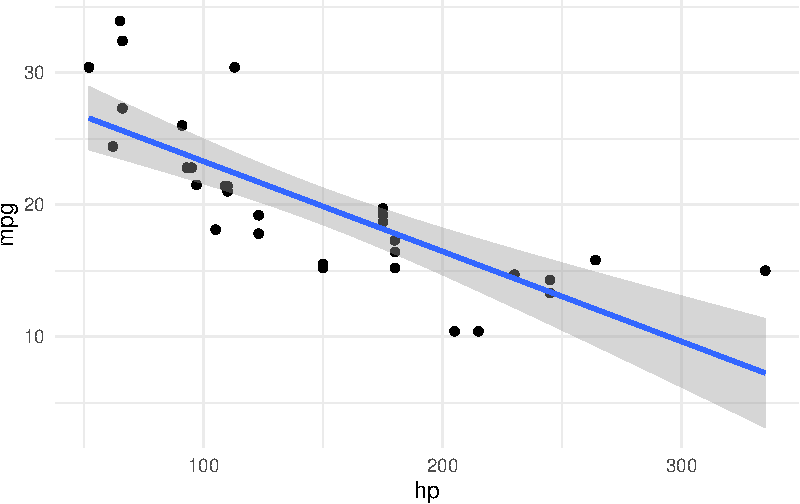
\includegraphics{./regression1_files/figure-pdf/in-all-its-glory-1.pdf}

\hypertarget{first-model-one-metric-predictor}{%
\section{First model: one metric
predictor}\label{first-model-one-metric-predictor}}

First, let's load some data:

\begin{Shaded}
\begin{Highlighting}[]
\FunctionTok{data}\NormalTok{(mtcars)}
\FunctionTok{glimpse}\NormalTok{(mtcars)}
\end{Highlighting}
\end{Shaded}

\begin{verbatim}
Rows: 32
Columns: 11
$ mpg  <dbl> 21.0, 21.0, 22.8, 21.4, 18.7, 18.1, 14.3, 24.4, 22.8, 19.2, 17.8,~
$ cyl  <dbl> 6, 6, 4, 6, 8, 6, 8, 4, 4, 6, 6, 8, 8, 8, 8, 8, 8, 4, 4, 4, 4, 8,~
$ disp <dbl> 160.0, 160.0, 108.0, 258.0, 360.0, 225.0, 360.0, 146.7, 140.8, 16~
$ hp   <dbl> 110, 110, 93, 110, 175, 105, 245, 62, 95, 123, 123, 180, 180, 180~
$ drat <dbl> 3.90, 3.90, 3.85, 3.08, 3.15, 2.76, 3.21, 3.69, 3.92, 3.92, 3.92,~
$ wt   <dbl> 2.620, 2.875, 2.320, 3.215, 3.440, 3.460, 3.570, 3.190, 3.150, 3.~
$ qsec <dbl> 16.46, 17.02, 18.61, 19.44, 17.02, 20.22, 15.84, 20.00, 22.90, 18~
$ vs   <dbl> 0, 0, 1, 1, 0, 1, 0, 1, 1, 1, 1, 0, 0, 0, 0, 0, 0, 1, 1, 1, 1, 0,~
$ am   <dbl> 1, 1, 1, 0, 0, 0, 0, 0, 0, 0, 0, 0, 0, 0, 0, 0, 0, 1, 1, 1, 0, 0,~
$ gear <dbl> 4, 4, 4, 3, 3, 3, 3, 4, 4, 4, 4, 3, 3, 3, 3, 3, 3, 4, 4, 4, 3, 3,~
$ carb <dbl> 4, 4, 1, 1, 2, 1, 4, 2, 2, 4, 4, 3, 3, 3, 4, 4, 4, 1, 2, 1, 1, 2,~
\end{verbatim}

\hypertarget{frequentist}{%
\subsection{Frequentist}\label{frequentist}}

Define and fit the model:

\begin{Shaded}
\begin{Highlighting}[]
\NormalTok{lm1\_freq }\OtherTok{\textless{}{-}} \FunctionTok{lm}\NormalTok{(mpg }\SpecialCharTok{\textasciitilde{}}\NormalTok{ hp, }\AttributeTok{data =}\NormalTok{ mtcars)}
\end{Highlighting}
\end{Shaded}

Get the parameter values:

\begin{Shaded}
\begin{Highlighting}[]
\FunctionTok{parameters}\NormalTok{(lm1\_freq)}
\end{Highlighting}
\end{Shaded}

\begin{verbatim}
Parameter   | Coefficient |   SE |         95% CI | t(30) |      p
------------------------------------------------------------------
(Intercept) |       30.10 | 1.63 | [26.76, 33.44] | 18.42 | < .001
hp          |       -0.07 | 0.01 | [-0.09, -0.05] | -6.74 | < .001
\end{verbatim}

Plot the model parameters:

\begin{Shaded}
\begin{Highlighting}[]
\FunctionTok{plot}\NormalTok{(}\FunctionTok{parameters}\NormalTok{(lm1\_freq))}
\end{Highlighting}
\end{Shaded}

\begin{figure}[H]

{\centering 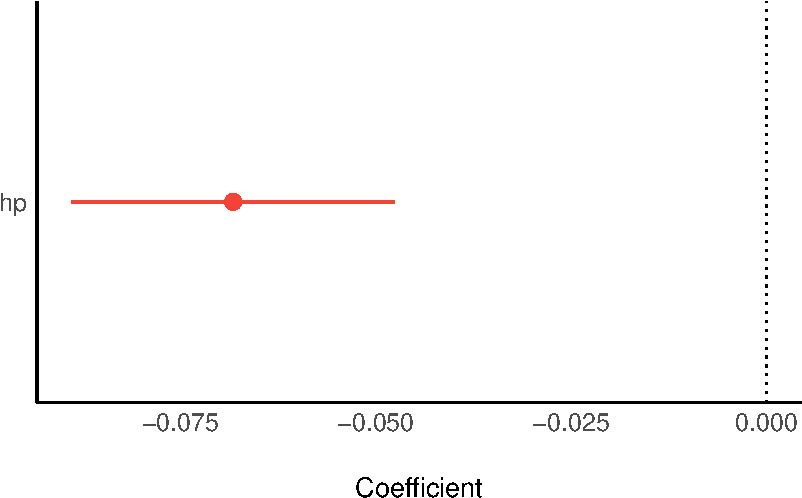
\includegraphics{./regression1_files/figure-pdf/plot-lm1-freq-1.pdf}

}

\end{figure}

\hypertarget{bayesian}{%
\subsection{Bayesian}\label{bayesian}}

\begin{Shaded}
\begin{Highlighting}[]
\NormalTok{lm1\_bayes }\OtherTok{\textless{}{-}} \FunctionTok{stan\_glm}\NormalTok{(mpg }\SpecialCharTok{\textasciitilde{}}\NormalTok{ hp, }\AttributeTok{data =}\NormalTok{ mtcars)}
\end{Highlighting}
\end{Shaded}

\begin{verbatim}

SAMPLING FOR MODEL 'continuous' NOW (CHAIN 1).
Chain 1: 
Chain 1: Gradient evaluation took 0.000671 seconds
Chain 1: 1000 transitions using 10 leapfrog steps per transition would take 6.71 seconds.
Chain 1: Adjust your expectations accordingly!
Chain 1: 
Chain 1: 
Chain 1: Iteration:    1 / 2000 [  0%]  (Warmup)
Chain 1: Iteration:  200 / 2000 [ 10%]  (Warmup)
Chain 1: Iteration:  400 / 2000 [ 20%]  (Warmup)
Chain 1: Iteration:  600 / 2000 [ 30%]  (Warmup)
Chain 1: Iteration:  800 / 2000 [ 40%]  (Warmup)
Chain 1: Iteration: 1000 / 2000 [ 50%]  (Warmup)
Chain 1: Iteration: 1001 / 2000 [ 50%]  (Sampling)
Chain 1: Iteration: 1200 / 2000 [ 60%]  (Sampling)
Chain 1: Iteration: 1400 / 2000 [ 70%]  (Sampling)
Chain 1: Iteration: 1600 / 2000 [ 80%]  (Sampling)
Chain 1: Iteration: 1800 / 2000 [ 90%]  (Sampling)
Chain 1: Iteration: 2000 / 2000 [100%]  (Sampling)
Chain 1: 
Chain 1:  Elapsed Time: 0.031964 seconds (Warm-up)
Chain 1:                0.030428 seconds (Sampling)
Chain 1:                0.062392 seconds (Total)
Chain 1: 

SAMPLING FOR MODEL 'continuous' NOW (CHAIN 2).
Chain 2: 
Chain 2: Gradient evaluation took 1.4e-05 seconds
Chain 2: 1000 transitions using 10 leapfrog steps per transition would take 0.14 seconds.
Chain 2: Adjust your expectations accordingly!
Chain 2: 
Chain 2: 
Chain 2: Iteration:    1 / 2000 [  0%]  (Warmup)
Chain 2: Iteration:  200 / 2000 [ 10%]  (Warmup)
Chain 2: Iteration:  400 / 2000 [ 20%]  (Warmup)
Chain 2: Iteration:  600 / 2000 [ 30%]  (Warmup)
Chain 2: Iteration:  800 / 2000 [ 40%]  (Warmup)
Chain 2: Iteration: 1000 / 2000 [ 50%]  (Warmup)
Chain 2: Iteration: 1001 / 2000 [ 50%]  (Sampling)
Chain 2: Iteration: 1200 / 2000 [ 60%]  (Sampling)
Chain 2: Iteration: 1400 / 2000 [ 70%]  (Sampling)
Chain 2: Iteration: 1600 / 2000 [ 80%]  (Sampling)
Chain 2: Iteration: 1800 / 2000 [ 90%]  (Sampling)
Chain 2: Iteration: 2000 / 2000 [100%]  (Sampling)
Chain 2: 
Chain 2:  Elapsed Time: 0.032053 seconds (Warm-up)
Chain 2:                0.030316 seconds (Sampling)
Chain 2:                0.062369 seconds (Total)
Chain 2: 

SAMPLING FOR MODEL 'continuous' NOW (CHAIN 3).
Chain 3: 
Chain 3: Gradient evaluation took 1.7e-05 seconds
Chain 3: 1000 transitions using 10 leapfrog steps per transition would take 0.17 seconds.
Chain 3: Adjust your expectations accordingly!
Chain 3: 
Chain 3: 
Chain 3: Iteration:    1 / 2000 [  0%]  (Warmup)
Chain 3: Iteration:  200 / 2000 [ 10%]  (Warmup)
Chain 3: Iteration:  400 / 2000 [ 20%]  (Warmup)
Chain 3: Iteration:  600 / 2000 [ 30%]  (Warmup)
Chain 3: Iteration:  800 / 2000 [ 40%]  (Warmup)
Chain 3: Iteration: 1000 / 2000 [ 50%]  (Warmup)
Chain 3: Iteration: 1001 / 2000 [ 50%]  (Sampling)
Chain 3: Iteration: 1200 / 2000 [ 60%]  (Sampling)
Chain 3: Iteration: 1400 / 2000 [ 70%]  (Sampling)
Chain 3: Iteration: 1600 / 2000 [ 80%]  (Sampling)
Chain 3: Iteration: 1800 / 2000 [ 90%]  (Sampling)
Chain 3: Iteration: 2000 / 2000 [100%]  (Sampling)
Chain 3: 
Chain 3:  Elapsed Time: 0.030275 seconds (Warm-up)
Chain 3:                0.03358 seconds (Sampling)
Chain 3:                0.063855 seconds (Total)
Chain 3: 

SAMPLING FOR MODEL 'continuous' NOW (CHAIN 4).
Chain 4: 
Chain 4: Gradient evaluation took 1.6e-05 seconds
Chain 4: 1000 transitions using 10 leapfrog steps per transition would take 0.16 seconds.
Chain 4: Adjust your expectations accordingly!
Chain 4: 
Chain 4: 
Chain 4: Iteration:    1 / 2000 [  0%]  (Warmup)
Chain 4: Iteration:  200 / 2000 [ 10%]  (Warmup)
Chain 4: Iteration:  400 / 2000 [ 20%]  (Warmup)
Chain 4: Iteration:  600 / 2000 [ 30%]  (Warmup)
Chain 4: Iteration:  800 / 2000 [ 40%]  (Warmup)
Chain 4: Iteration: 1000 / 2000 [ 50%]  (Warmup)
Chain 4: Iteration: 1001 / 2000 [ 50%]  (Sampling)
Chain 4: Iteration: 1200 / 2000 [ 60%]  (Sampling)
Chain 4: Iteration: 1400 / 2000 [ 70%]  (Sampling)
Chain 4: Iteration: 1600 / 2000 [ 80%]  (Sampling)
Chain 4: Iteration: 1800 / 2000 [ 90%]  (Sampling)
Chain 4: Iteration: 2000 / 2000 [100%]  (Sampling)
Chain 4: 
Chain 4:  Elapsed Time: 0.031825 seconds (Warm-up)
Chain 4:                0.029619 seconds (Sampling)
Chain 4:                0.061444 seconds (Total)
Chain 4: 
\end{verbatim}

Actually, we want to suppress some overly verbose output of the
sampling, so add the argument \texttt{refresh\ =\ 0}:

\begin{Shaded}
\begin{Highlighting}[]
\NormalTok{lm1\_bayes }\OtherTok{\textless{}{-}} \FunctionTok{stan\_glm}\NormalTok{(mpg }\SpecialCharTok{\textasciitilde{}}\NormalTok{ hp, }\AttributeTok{data =}\NormalTok{ mtcars, }\AttributeTok{refresh =} \DecValTok{0}\NormalTok{)}
\end{Highlighting}
\end{Shaded}

Get the parameter values:

\begin{Shaded}
\begin{Highlighting}[]
\FunctionTok{parameters}\NormalTok{(lm1\_bayes)}
\end{Highlighting}
\end{Shaded}

\begin{verbatim}
Parameter   | Median |         95% CI |   pd | % in ROPE |  Rhat |     ESS |                   Prior
----------------------------------------------------------------------------------------------------
(Intercept) |  30.12 | [26.85, 33.34] | 100% |        0% | 1.001 | 3257.00 | Normal (20.09 +- 15.07)
hp          |  -0.07 | [-0.09, -0.05] | 100% |      100% | 1.000 | 3387.00 |   Normal (0.00 +- 0.22)
\end{verbatim}

Plot the model parameters:

\begin{Shaded}
\begin{Highlighting}[]
\FunctionTok{plot}\NormalTok{(}\FunctionTok{parameters}\NormalTok{(lm1\_bayes))}
\end{Highlighting}
\end{Shaded}

\begin{figure}[H]

{\centering 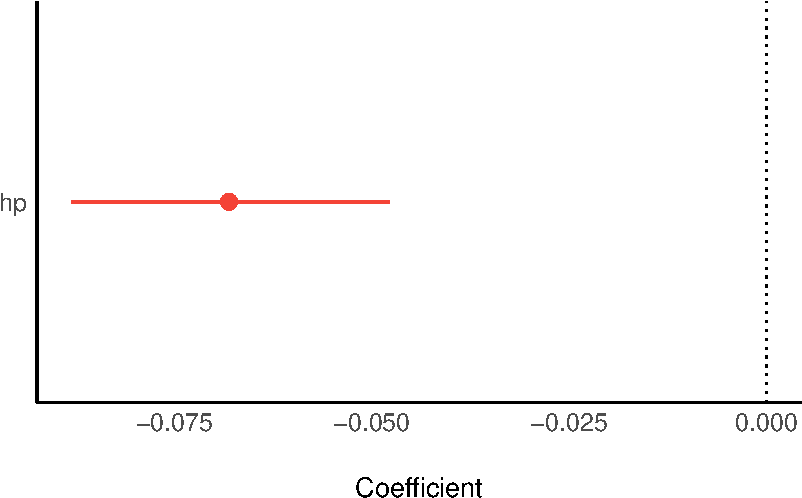
\includegraphics{./regression1_files/figure-pdf/unnamed-chunk-4-1.pdf}

}

\end{figure}

\hypertarget{model-performance}{%
\subsection{Model performance}\label{model-performance}}

\begin{Shaded}
\begin{Highlighting}[]
\FunctionTok{r2}\NormalTok{(lm1\_freq)}
\end{Highlighting}
\end{Shaded}

\begin{verbatim}
# R2 for Linear Regression
       R2: 0.602
  adj. R2: 0.589
\end{verbatim}

\begin{Shaded}
\begin{Highlighting}[]
\FunctionTok{r2}\NormalTok{(lm1\_bayes)}
\end{Highlighting}
\end{Shaded}

\begin{verbatim}
# Bayesian R2 with Compatibility Interval

  Conditional R2: 0.585 (95% CI [0.376, 0.744])
\end{verbatim}

\hypertarget{model-check}{%
\subsection{Model check}\label{model-check}}

Here's a bunch of typical model checks in the Frequentist sense.

\begin{Shaded}
\begin{Highlighting}[]
\FunctionTok{check\_model}\NormalTok{(lm1\_freq)}
\end{Highlighting}
\end{Shaded}

\begin{figure}[H]

{\centering 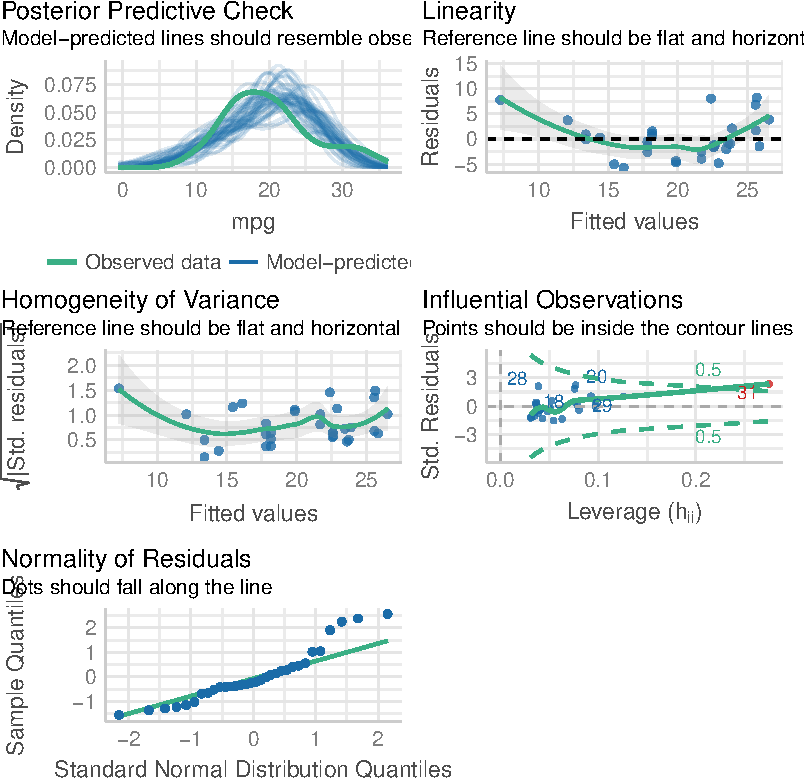
\includegraphics[width=1\textwidth,height=\textheight]{./regression1_files/figure-pdf/checkmodel-lm1-freq-1.pdf}

}

\end{figure}

And here are some Bayesian flavored model checks.

\begin{Shaded}
\begin{Highlighting}[]
\FunctionTok{check\_model}\NormalTok{(lm1\_bayes)}
\end{Highlighting}
\end{Shaded}

\begin{figure}[H]

{\centering 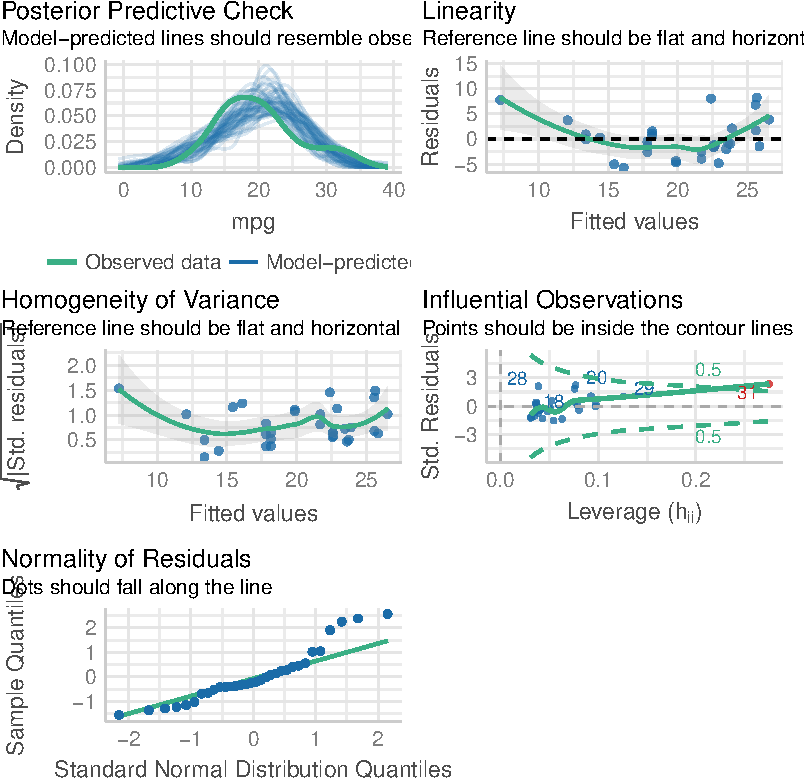
\includegraphics[width=1\textwidth,height=\textheight]{./regression1_files/figure-pdf/checkmodel-lm1-bayes-1.pdf}

}

\end{figure}

\hypertarget{get-some-predictions}{%
\subsection{Get some predictions}\label{get-some-predictions}}

\begin{Shaded}
\begin{Highlighting}[]
\NormalTok{lm1\_pred }\OtherTok{\textless{}{-}} \FunctionTok{estimate\_relation}\NormalTok{(lm1\_freq)}
\NormalTok{lm1\_pred}
\end{Highlighting}
\end{Shaded}

\begin{verbatim}
Model-based Expectation

hp     | Predicted |   SE |         95% CI
------------------------------------------
52.00  |     26.55 | 1.18 | [24.15, 28.95]
83.44  |     24.41 | 0.94 | [22.49, 26.32]
114.89 |     22.26 | 0.75 | [20.72, 23.80]
146.33 |     20.11 | 0.68 | [18.72, 21.51]
177.78 |     17.97 | 0.75 | [16.43, 19.50]
209.22 |     15.82 | 0.93 | [13.92, 17.73]
240.67 |     13.68 | 1.17 | [11.29, 16.07]
272.11 |     11.53 | 1.44 | [ 8.59, 14.48]
303.56 |      9.39 | 1.73 | [ 5.86, 12.92]
335.00 |      7.24 | 2.02 | [ 3.11, 11.38]

Variable predicted: mpg
Predictors modulated: hp
\end{verbatim}

More details on the above function can be found on the
\href{https://easystats.github.io/modelbased/reference/estimate_expectation.html\#functions-for-estimating-predicted-values-and-uncertainty}{respective
page at the easystats site}.

\hypertarget{plot-the-model}{%
\subsection{Plot the model}\label{plot-the-model}}

\begin{Shaded}
\begin{Highlighting}[]
\FunctionTok{plot}\NormalTok{(lm1\_pred)}
\end{Highlighting}
\end{Shaded}

\begin{figure}[H]

{\centering 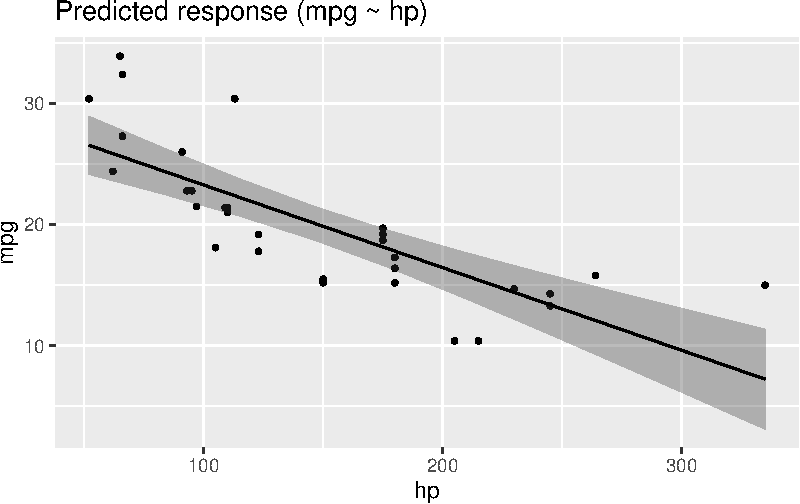
\includegraphics{./regression1_files/figure-pdf/plot-lm1-pred-1.pdf}

}

\end{figure}

\hypertarget{more-of-this}{%
\section{More of this}\label{more-of-this}}

More technical details for gauging model performance and model quality,
can be found on the site of
\href{https://easystats.github.io/performance/}{the R package
``performance} at the easystats site.

\hypertarget{bayes-members-only}{%
\section{Bayes-members only}\label{bayes-members-only}}

Bayes statistics provide a distribution as the result of the analysis,
the posterior distribution, which provides us with quite some luxury.

As the posterior distribution manifests itself by a number of samples,
we can easily filter and manipulate this sample distribution in order to
ask some interesing questions.

See:

\begin{Shaded}
\begin{Highlighting}[]
\NormalTok{lm1\_bayes }\SpecialCharTok{\%\textgreater{}\%} 
  \FunctionTok{as\_tibble}\NormalTok{() }\SpecialCharTok{\%\textgreater{}\%} 
  \FunctionTok{head}\NormalTok{()}
\end{Highlighting}
\end{Shaded}

\begin{verbatim}
# A tibble: 6 x 3
  `(Intercept)`      hp sigma
          <dbl>   <dbl> <dbl>
1          27.5 -0.0545  3.86
2          32.4 -0.0812  3.60
3          29.7 -0.0567  3.86
4          29.5 -0.0608  4.47
5          30.7 -0.0664  3.78
6          29.4 -0.0682  3.89
\end{verbatim}

\hypertarget{asking-for-probabilites}{%
\subsection{Asking for probabilites}\label{asking-for-probabilites}}

\emph{What's the probability that the effect of hp is negative?}

\begin{Shaded}
\begin{Highlighting}[]
\NormalTok{lm1\_bayes }\SpecialCharTok{\%\textgreater{}\%} 
  \FunctionTok{as\_tibble}\NormalTok{() }\SpecialCharTok{\%\textgreater{}\%} 
  \FunctionTok{count}\NormalTok{(hp }\SpecialCharTok{\textless{}} \DecValTok{0}\NormalTok{)}
\end{Highlighting}
\end{Shaded}

\begin{verbatim}
# A tibble: 1 x 2
  `hp < 0`     n
  <lgl>    <int>
1 TRUE      4000
\end{verbatim}

Feel free to ask similar questions!

\hypertarget{asking-for-quantiles}{%
\subsection{Asking for quantiles}\label{asking-for-quantiles}}

\emph{With a given probability of, say 90\%, how large is the effect of
hp?}

\begin{Shaded}
\begin{Highlighting}[]
\NormalTok{lm1\_bayes }\SpecialCharTok{\%\textgreater{}\%} 
  \FunctionTok{as\_tibble}\NormalTok{() }\SpecialCharTok{\%\textgreater{}\%} 
  \FunctionTok{summarise}\NormalTok{(}\AttributeTok{q\_90 =} \FunctionTok{quantile}\NormalTok{(hp, .}\DecValTok{9}\NormalTok{))}
\end{Highlighting}
\end{Shaded}

\begin{verbatim}
# A tibble: 1 x 1
     q_90
    <dbl>
1 -0.0550
\end{verbatim}

\emph{What's the smallest 95\% percent interval for the effect of hp?}

\begin{Shaded}
\begin{Highlighting}[]
\FunctionTok{hdi}\NormalTok{(lm1\_bayes)}
\end{Highlighting}
\end{Shaded}

\begin{verbatim}
Highest Density Interval

Parameter   |        95% HDI
----------------------------
(Intercept) | [26.95, 33.43]
hp          | [-0.09, -0.05]
\end{verbatim}

In case you prefer 89\% intervals (I do!):

\begin{Shaded}
\begin{Highlighting}[]
\FunctionTok{hdi}\NormalTok{(lm1\_bayes, }\AttributeTok{ci =}\NormalTok{ .}\DecValTok{89}\NormalTok{)}
\end{Highlighting}
\end{Shaded}

\begin{verbatim}
Highest Density Interval

Parameter   |        89% HDI
----------------------------
(Intercept) | [27.41, 32.68]
hp          | [-0.09, -0.05]
\end{verbatim}

\hypertarget{multiple-metric-predictors}{%
\section{Multiple metric predictors}\label{multiple-metric-predictors}}

Assume we have a theory that dictates that fuel economy is a (causal)
function of horse power and engine displacement.

\begin{Shaded}
\begin{Highlighting}[]
\NormalTok{lm2\_freq }\OtherTok{\textless{}{-}} \FunctionTok{lm}\NormalTok{(mpg }\SpecialCharTok{\textasciitilde{}}\NormalTok{ hp }\SpecialCharTok{+}\NormalTok{ disp, }\AttributeTok{data =}\NormalTok{ mtcars)}
\FunctionTok{parameters}\NormalTok{(lm2\_freq)}
\end{Highlighting}
\end{Shaded}

\begin{verbatim}
Parameter   | Coefficient |       SE |         95% CI | t(29) |      p
----------------------------------------------------------------------
(Intercept) |       30.74 |     1.33 | [28.01, 33.46] | 23.08 | < .001
hp          |       -0.02 |     0.01 | [-0.05,  0.00] | -1.86 | 0.074 
disp        |       -0.03 | 7.40e-03 | [-0.05, -0.02] | -4.10 | < .001
\end{verbatim}

Similarly for Bayes inference:

\begin{Shaded}
\begin{Highlighting}[]
\NormalTok{lm2\_bayes }\OtherTok{\textless{}{-}} \FunctionTok{stan\_glm}\NormalTok{(mpg }\SpecialCharTok{\textasciitilde{}}\NormalTok{ hp }\SpecialCharTok{+}\NormalTok{ disp, }\AttributeTok{data =}\NormalTok{ mtcars)}
\end{Highlighting}
\end{Shaded}

Results

\begin{Shaded}
\begin{Highlighting}[]
\FunctionTok{parameters}\NormalTok{(lm2\_bayes)}
\end{Highlighting}
\end{Shaded}

\begin{verbatim}
Parameter   | Median |         95% CI |     pd | % in ROPE |  Rhat |     ESS |                   Prior
------------------------------------------------------------------------------------------------------
(Intercept) |  30.78 | [27.94, 33.57] |   100% |        0% | 0.999 | 5095.00 | Normal (20.09 +- 15.07)
hp          |  -0.02 | [-0.05,  0.00] | 97.28% |      100% | 1.001 | 2226.00 |   Normal (0.00 +- 0.22)
disp        |  -0.03 | [-0.04, -0.01] |   100% |      100% | 1.001 | 2150.00 |   Normal (0.00 +- 0.12)
\end{verbatim}

\begin{Shaded}
\begin{Highlighting}[]
\FunctionTok{plot}\NormalTok{(}\FunctionTok{parameters}\NormalTok{(lm2\_bayes))}
\end{Highlighting}
\end{Shaded}

\begin{figure}[H]

{\centering 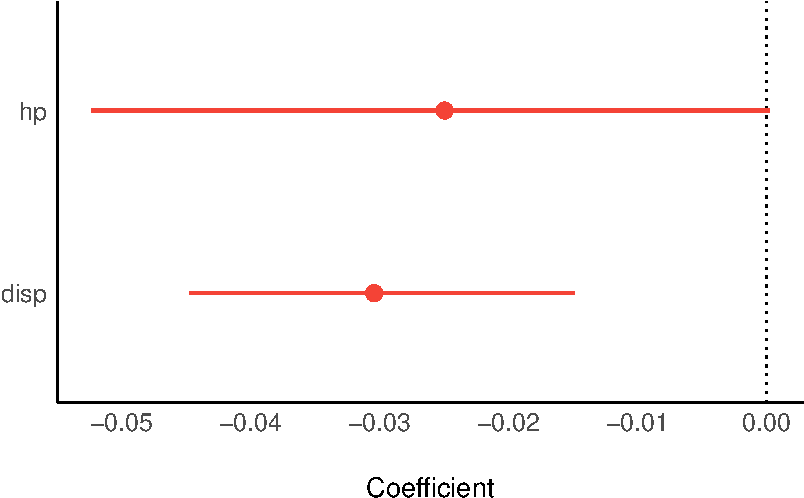
\includegraphics{./regression1_files/figure-pdf/lm2-results-1.pdf}

}

\end{figure}

\begin{Shaded}
\begin{Highlighting}[]
\FunctionTok{r2}\NormalTok{(lm2\_bayes)}
\end{Highlighting}
\end{Shaded}

\begin{verbatim}
# Bayesian R2 with Compatibility Interval

  Conditional R2: 0.731 (95% CI [0.579, 0.847])
\end{verbatim}

Depending on the value of \texttt{disp} the prediction of \texttt{mpg}
from \texttt{hp} will vary:

\begin{Shaded}
\begin{Highlighting}[]
\NormalTok{lm2\_pred }\OtherTok{\textless{}{-}} \FunctionTok{estimate\_relation}\NormalTok{(lm2\_freq)}
\FunctionTok{plot}\NormalTok{(lm2\_pred)}
\end{Highlighting}
\end{Shaded}

\begin{figure}[H]

{\centering 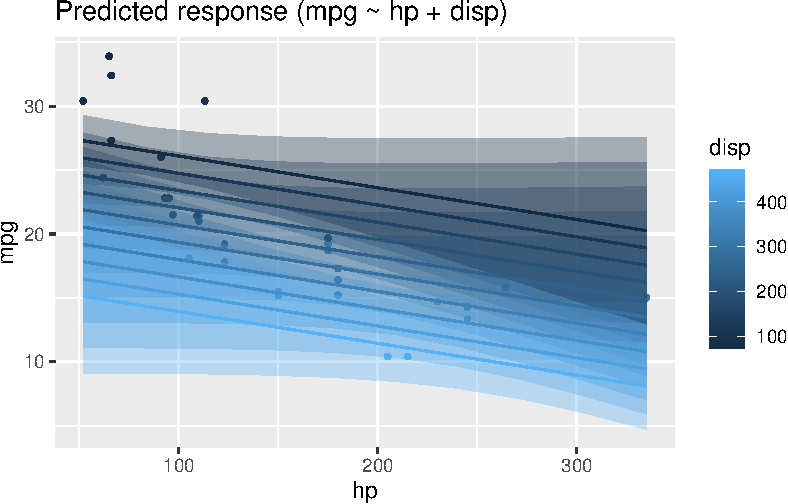
\includegraphics{./regression1_files/figure-pdf/lm2-pred-1.pdf}

}

\end{figure}

\hypertarget{one-nominal-predictor}{%
\section{One nominal predictor}\label{one-nominal-predictor}}

\begin{Shaded}
\begin{Highlighting}[]
\NormalTok{lm3a }\OtherTok{\textless{}{-}} \FunctionTok{lm}\NormalTok{(mpg }\SpecialCharTok{\textasciitilde{}}\NormalTok{ am, }\AttributeTok{data =}\NormalTok{ mtcars)}
\FunctionTok{parameters}\NormalTok{(lm3a)}
\end{Highlighting}
\end{Shaded}

\begin{verbatim}
Parameter   | Coefficient |   SE |         95% CI | t(30) |      p
------------------------------------------------------------------
(Intercept) |       17.15 | 1.12 | [14.85, 19.44] | 15.25 | < .001
am          |        7.24 | 1.76 | [ 3.64, 10.85] |  4.11 | < .001
\end{verbatim}

\begin{Shaded}
\begin{Highlighting}[]
\NormalTok{lm3a\_means }\OtherTok{\textless{}{-}} \FunctionTok{estimate\_means}\NormalTok{(lm3a, }\AttributeTok{at =} \StringTok{"am = c(0, 1)"}\NormalTok{)}
\NormalTok{lm3a\_means }
\end{Highlighting}
\end{Shaded}

\begin{verbatim}
Estimated Marginal Means

am   |  Mean |   SE |         95% CI
------------------------------------
0.00 | 17.15 | 1.12 | [14.85, 19.44]
1.00 | 24.39 | 1.36 | [21.62, 27.17]

Marginal means estimated at am
\end{verbatim}

If we were not to specify the values of \texttt{am} which we would like
to get predictions for, the default of the function would select 10
values, spreaded across the range of \texttt{am}. For numeric variables,
this is usually fine. However, for nominal variables - and \texttt{am}
is in fact a nominally scaled variable - we insist that we want
predictions for the levels of the variable only, that is for \texttt{0}
and \texttt{1}.

However, unfortunately, the plot \emph{needs} a nominal variable if we
are to compare groups. In our case, \texttt{am} is considered a numeric
variables, since it consists of numbers only. The plot does not work,
malheureusement:

\begin{Shaded}
\begin{Highlighting}[]
\FunctionTok{plot}\NormalTok{(lm3a\_means)}
\end{Highlighting}
\end{Shaded}

\begin{figure}[H]

{\centering 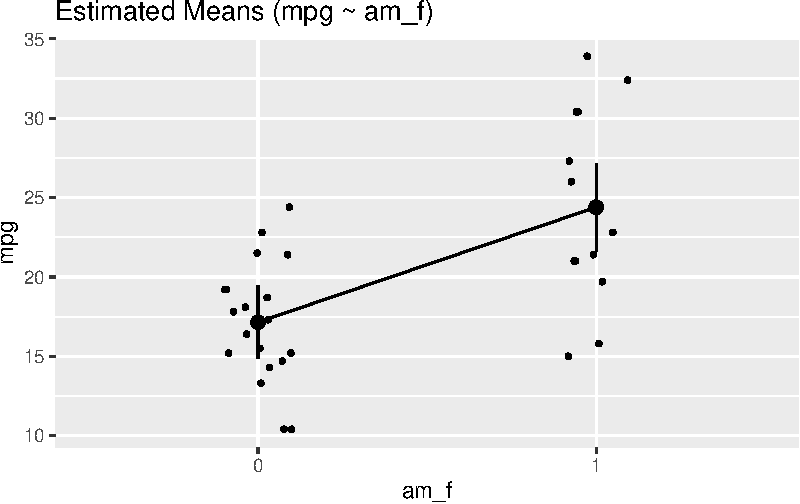
\includegraphics{./regression1_files/figure-pdf/unnamed-chunk-12-1.pdf}

}

\end{figure}

We need to transform \texttt{am} to a factor variable. That's something
like a string. If we hand over a \texttt{factor()} to the plotting
function, everything will run smoothly. Computationwise, no big
differences:

\begin{Shaded}
\begin{Highlighting}[]
\NormalTok{mtcars2 }\OtherTok{\textless{}{-}}
\NormalTok{  mtcars }\SpecialCharTok{\%\textgreater{}\%} 
  \FunctionTok{mutate}\NormalTok{(}\AttributeTok{am\_f =} \FunctionTok{factor}\NormalTok{(am))}

\NormalTok{lm3a }\OtherTok{\textless{}{-}} \FunctionTok{lm}\NormalTok{(mpg }\SpecialCharTok{\textasciitilde{}}\NormalTok{ am\_f, }\AttributeTok{data =}\NormalTok{ mtcars2)}
\FunctionTok{parameters}\NormalTok{(lm3a)}
\end{Highlighting}
\end{Shaded}

\begin{verbatim}
Parameter   | Coefficient |   SE |         95% CI | t(30) |      p
------------------------------------------------------------------
(Intercept) |       17.15 | 1.12 | [14.85, 19.44] | 15.25 | < .001
am f [1]    |        7.24 | 1.76 | [ 3.64, 10.85] |  4.11 | < .001
\end{verbatim}

\begin{Shaded}
\begin{Highlighting}[]
\NormalTok{lm3a\_means }\OtherTok{\textless{}{-}} \FunctionTok{estimate\_means}\NormalTok{(lm3a)}
\FunctionTok{plot}\NormalTok{(lm3a\_means)}
\end{Highlighting}
\end{Shaded}

\begin{figure}[H]

{\centering 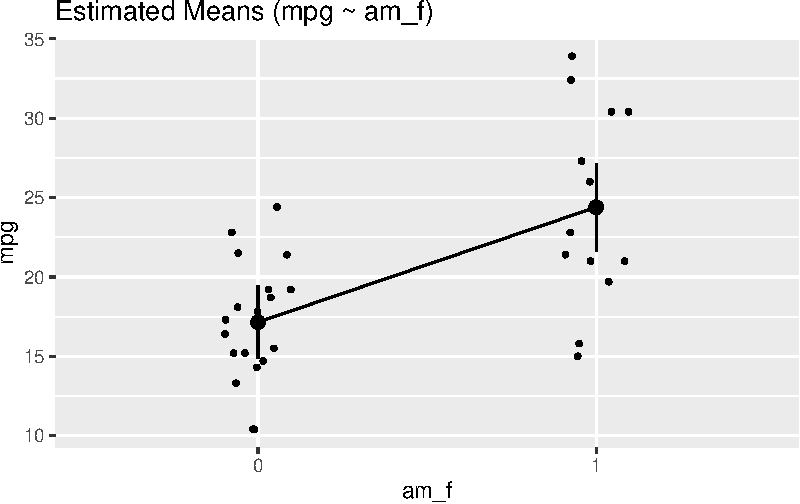
\includegraphics{./regression1_files/figure-pdf/unnamed-chunk-13-1.pdf}

}

\end{figure}

Note that we should have converted \texttt{am} to a factor variable
before fitting the model. Otherwise, the plot won't work.

Here's a more hand-crafted version of the last plot, see Fig.
Figure~\ref{fig-lm3a-means}.

\begin{Shaded}
\begin{Highlighting}[]
\FunctionTok{ggplot}\NormalTok{(mtcars2) }\SpecialCharTok{+}
  \FunctionTok{aes}\NormalTok{(}\AttributeTok{x =}\NormalTok{ am\_f, }\AttributeTok{y =}\NormalTok{ mpg) }\SpecialCharTok{+}
  \FunctionTok{geom\_violin}\NormalTok{() }\SpecialCharTok{+}
  \FunctionTok{geom\_jitter}\NormalTok{(}\AttributeTok{width =}\NormalTok{ .}\DecValTok{1}\NormalTok{, }\AttributeTok{alpha =}\NormalTok{ .}\DecValTok{5}\NormalTok{) }\SpecialCharTok{+}
  \FunctionTok{geom\_pointrange}\NormalTok{(}\AttributeTok{data =}\NormalTok{ lm3a\_means,}
                  \AttributeTok{color =} \StringTok{"orange"}\NormalTok{,}
                  \FunctionTok{aes}\NormalTok{(}\AttributeTok{ymin =}\NormalTok{ CI\_low, }\AttributeTok{ymax =}\NormalTok{ CI\_high, }\AttributeTok{y =}\NormalTok{ Mean)) }\SpecialCharTok{+}
  \FunctionTok{geom\_line}\NormalTok{(}\AttributeTok{data =}\NormalTok{ lm3a\_means, }\FunctionTok{aes}\NormalTok{(}\AttributeTok{y =}\NormalTok{ Mean, }\AttributeTok{group =} \DecValTok{1}\NormalTok{))}
\end{Highlighting}
\end{Shaded}

\begin{figure}[H]

{\centering 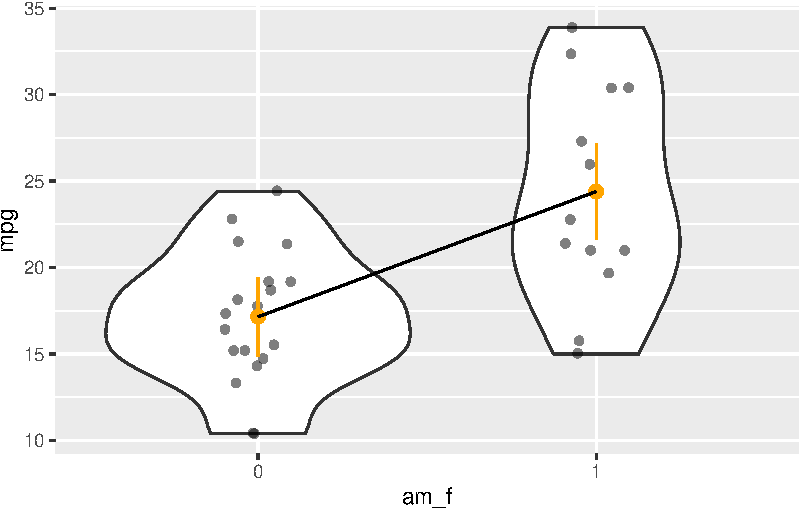
\includegraphics{./regression1_files/figure-pdf/fig-lm3a-means-1.pdf}

}

\caption{\label{fig-lm3a-means}\textbf{?(caption)}}

\end{figure}

\hypertarget{one-metric-and-one-nominal-predictor}{%
\section{One metric and one nominal
predictor}\label{one-metric-and-one-nominal-predictor}}

\begin{Shaded}
\begin{Highlighting}[]
\NormalTok{mtcars2 }\OtherTok{\textless{}{-}}
\NormalTok{  mtcars }\SpecialCharTok{\%\textgreater{}\%} 
  \FunctionTok{mutate}\NormalTok{(}\AttributeTok{cyl =} \FunctionTok{factor}\NormalTok{(cyl))}

\NormalTok{lm4 }\OtherTok{\textless{}{-}} \FunctionTok{lm}\NormalTok{(mpg }\SpecialCharTok{\textasciitilde{}}\NormalTok{ hp }\SpecialCharTok{+}\NormalTok{ cyl, }\AttributeTok{data =}\NormalTok{ mtcars2)}
\FunctionTok{parameters}\NormalTok{(lm4)}
\end{Highlighting}
\end{Shaded}

\begin{verbatim}
Parameter   | Coefficient |   SE |          95% CI | t(28) |      p
-------------------------------------------------------------------
(Intercept) |       28.65 | 1.59 | [ 25.40, 31.90] | 18.04 | < .001
hp          |       -0.02 | 0.02 | [ -0.06,  0.01] | -1.56 | 0.130 
cyl [6]     |       -5.97 | 1.64 | [ -9.33, -2.61] | -3.64 | 0.001 
cyl [8]     |       -8.52 | 2.33 | [-13.29, -3.76] | -3.66 | 0.001 
\end{verbatim}

\begin{Shaded}
\begin{Highlighting}[]
\NormalTok{lm4\_pred }\OtherTok{\textless{}{-}} \FunctionTok{estimate\_relation}\NormalTok{(lm4)}
\FunctionTok{plot}\NormalTok{(lm4\_pred)}
\end{Highlighting}
\end{Shaded}

\begin{figure}[H]

{\centering 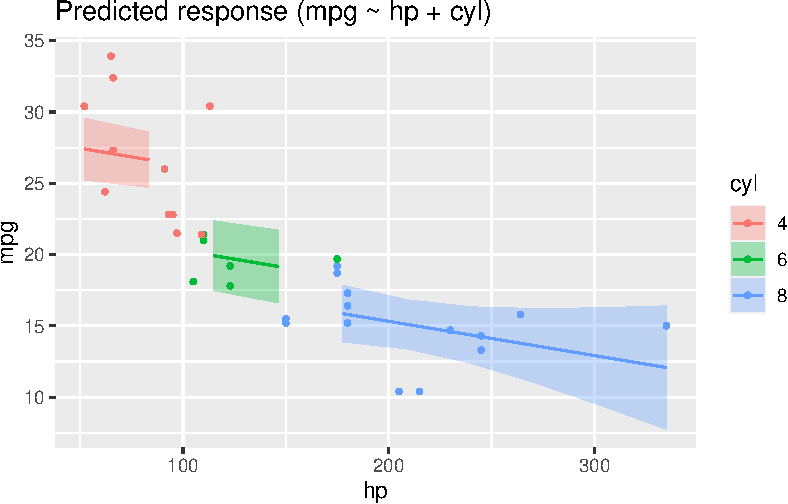
\includegraphics{./regression1_files/figure-pdf/lm4-pred-1.pdf}

}

\end{figure}

\hypertarget{watch-out-for-simpson}{%
\section{Watch out for Simpson}\label{watch-out-for-simpson}}

Beware! Model estimates can swing wildly if you add (or remove) some
predictor from your model.
\href{https://ecologyforthemasses.com/2022/06/08/who-is-simpson-and-what-does-his-paradox-mean-for-ecologists/}{See
this post} for an demonstration.

\hypertarget{what-about-correlation}{%
\section{What about correlation?}\label{what-about-correlation}}

Correlation is really a close cousin to regression. In fact, regression
with standardized variables amounts to correlation.

Let's get the correlation matrix of the variables in involved in
\texttt{lm4}.

\begin{Shaded}
\begin{Highlighting}[]
\NormalTok{lm4\_corr }\OtherTok{\textless{}{-}} 
\NormalTok{  mtcars }\SpecialCharTok{\%\textgreater{}\%} 
  \FunctionTok{select}\NormalTok{(mpg, hp, disp) }\SpecialCharTok{\%\textgreater{}\%} 
  \FunctionTok{correlation}\NormalTok{()}

\NormalTok{lm4\_corr}
\end{Highlighting}
\end{Shaded}

\begin{verbatim}
# Correlation Matrix (pearson-method)

Parameter1 | Parameter2 |     r |         95% CI | t(30) |         p
--------------------------------------------------------------------
mpg        |         hp | -0.78 | [-0.89, -0.59] | -6.74 | < .001***
mpg        |       disp | -0.85 | [-0.92, -0.71] | -8.75 | < .001***
hp         |       disp |  0.79 | [ 0.61,  0.89] |  7.08 | < .001***

p-value adjustment method: Holm (1979)
Observations: 32
\end{verbatim}

\begin{Shaded}
\begin{Highlighting}[]
\FunctionTok{plot}\NormalTok{(}\FunctionTok{summary}\NormalTok{(lm4\_corr))}
\end{Highlighting}
\end{Shaded}

\begin{figure}[H]

{\centering 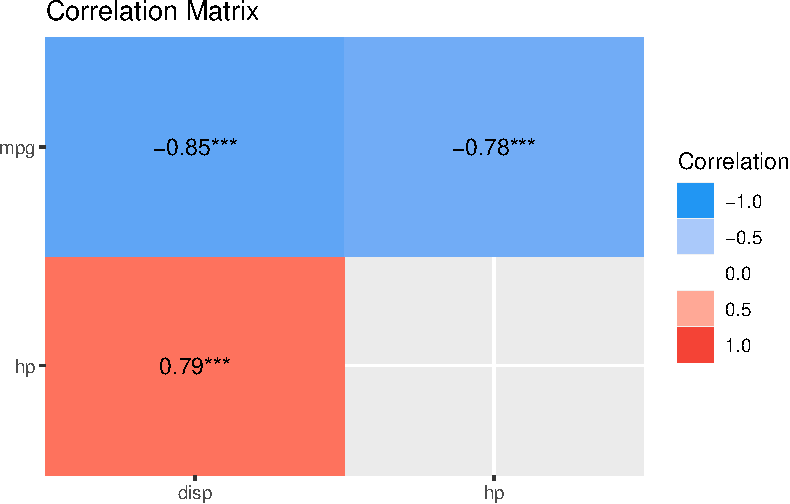
\includegraphics{./regression1_files/figure-pdf/unnamed-chunk-14-1.pdf}

}

\end{figure}

\hypertarget{exercises}{%
\section{Exercises}\label{exercises}}

\begin{enumerate}
\def\labelenumi{\arabic{enumi}.}
\tightlist
\item
  \href{https://datenwerk.netlify.app/posts/mtcars-simple1/mtcars-simple1/}{mtcars
  simple 1}
\item
  \href{https://datenwerk.netlify.app/posts/mtcars-simple2/mtcars-simple2/}{mtcars
  simple 2}
\item
  \href{https://datenwerk.netlify.app/posts/mtcars-simple3/mtcars-simple3/}{mtcars
  simple 3}
\end{enumerate}

\hypertarget{lab}{%
\section{Lab}\label{lab}}

Get your own data, and build a simple model reflecting your research
hypothesis. If you are lacking data (or hypothesis) get something close
to it.

\hypertarget{literature-2}{%
\section{Literature}\label{literature-2}}

An accessible treatment of regression is provided by Ismay and Kim
(2020).

Roback and Legler (2021) provide a more than introductory account of
regression while being accessible. A recent but already classic book (if
this is possible) is the book by Gelman, Hill, and Vehtari (2021). You
may also benefit from Poldrack (2022) (open access).

\hypertarget{debrief}{%
\section{Debrief}\label{debrief}}

\href{https://media.giphy.com/media/141amBdjqs9Vvy/giphy.gif}{Science!}

\bookmarksetup{startatroot}

\hypertarget{more-lineare-models}{%
\chapter{More lineare models}\label{more-lineare-models}}

\includegraphics[width=0.05\textwidth,height=\textheight]{./img/stern.png}

\hypertarget{r-packages-needed}{%
\section{R-packages needed}\label{r-packages-needed}}

\hypertarget{r-packages-needed-for-this-chapter-2}{%
\section{R packages needed for this
chapter}\label{r-packages-needed-for-this-chapter-2}}

\begin{Shaded}
\begin{Highlighting}[]
\FunctionTok{library}\NormalTok{(easystats)}
\FunctionTok{library}\NormalTok{(tidyverse)}
\end{Highlighting}
\end{Shaded}

\hypertarget{multiplicative-associations}{%
\section{Multiplicative
associations}\label{multiplicative-associations}}

\hypertarget{the-log-y-model}{%
\subsection{The Log-Y model}\label{the-log-y-model}}

Consider again the linear model, in a simple form:

\[\hat{y} = \beta_0 + \beta_1 x_1 +  \ldots + b_kx_k +\] Surprisingly,
we can use this \emph{linear} model to describe \emph{multiplicative}
assocations:

\(\hat{y} = e^{b_0 + b_1x_1 + b_2x_2 + \ldots + b_kx_k}\)

(I wrote \texttt{b} instead of \(\beta\) just to show that both has its
meaning, but are separate things.)

Exponentiate both sides to get:

\(log (\hat{y}) = b_0 + b_1x_1 + b_2x_2 + \ldots + b_kx_k\)

For simplicity, let's drop the subscripts in the following without loss
of generality and keep it short:

\(y = e^{x}\), with \(e \approx 2.71...\)

Exponentiate both sides to get:

\(log(y) = x\)

This association is called multiplicative, because if x increases by 1,
y increased by a \emph{constant factor}.

\begin{tcolorbox}[enhanced jigsaw, bottomrule=.15mm, toprule=.15mm, coltitle=black, breakable, title=\textcolor{quarto-callout-note-color}{\faInfo}\hspace{0.5em}{Note}, leftrule=.75mm, colback=white, bottomtitle=1mm, toptitle=1mm, left=2mm, opacityback=0, titlerule=0mm, colbacktitle=quarto-callout-note-color!10!white, opacitybacktitle=0.6, colframe=quarto-callout-note-color-frame, rightrule=.15mm, arc=.35mm]
The logarithm is not defined for negative (input) values. And
\(log(0) = -\infty\).
\end{tcolorbox}

A side-effect of modelling \texttt{log\_y} instead of \texttt{y} is that
the distribution shape of the outcome variable changes. This can be
useful at times.

Log-Y Regression can usefully be employed for modelling growth, among
othrs, see Example~\ref{exm-logy}.

\leavevmode\vadjust pre{\hypertarget{exm-logy}{}}%
\begin{example}[Bacteria growth]\label{exm-logy}

Some bacteria dish grows with at a fixed proportional rate, that is it
doubles its population size in a fixed period of time. This is what is
called exponential growth. For concreteness, say, the bacteriae double
each two days, starting with 1 unit of bacteria.

After about three weeks, we'll have this number (of units) of bacteriae:

\begin{Shaded}
\begin{Highlighting}[]
\NormalTok{e }\OtherTok{\textless{}{-}} \FloatTok{2.7178}
\NormalTok{e}\SpecialCharTok{\^{}}\DecValTok{10}
\end{Highlighting}
\end{Shaded}

\begin{verbatim}
[1] 21987.45
\end{verbatim}

\end{example}

\hypertarget{exercise}{%
\subsection{Exercise}\label{exercise}}

\begin{itemize}
\tightlist
\item
  \href{https://datenwerk.netlify.app/post/log-y-regr1/log-y-regr1/}{Effect
  of education on income}
\item
  \href{https://datenwerk.netlify.app/post/log-y-regr2/log-y-regr2/}{Effect
  of log-y transformation on the distribution, an example}
\end{itemize}

\begin{tcolorbox}[enhanced jigsaw, bottomrule=.15mm, toprule=.15mm, coltitle=black, breakable, title=\textcolor{quarto-callout-note-color}{\faInfo}\hspace{0.5em}{Note}, leftrule=.75mm, colback=white, bottomtitle=1mm, toptitle=1mm, left=2mm, opacityback=0, titlerule=0mm, colbacktitle=quarto-callout-note-color!10!white, opacitybacktitle=0.6, colframe=quarto-callout-note-color-frame, rightrule=.15mm, arc=.35mm]
The exercises are written in German Language. Don't fret. Browsers are
able to translate websites instantaneously. Alternatively, go to sites
such as
\href{https://translate.google.de/?sl=de\&tl=en\&op=websites}{Google
Translate} and enter the URL of the website to be translated. Also check
out the webstor of your favorite browser to get an extention
\href{https://chrome.google.com/webstore/detail/google-translate}{such
as this one for Google Chrome}.
\end{tcolorbox}

\hypertarget{visualizing-log-transformation}{%
\subsection{Visualizing Log
Transformation}\label{visualizing-log-transformation}}

Check out
\href{https://data-se.netlify.app/2022/01/14/visualizing-a-log-y-regression-model/}{this
post} for an example of a log-y regression visualized.

\href{https://data-se.netlify.app/2021/06/17/ein-beispiel-zum-nutzen-einer-log-transformation/}{This
post} puts some more weight to the argument that a log-y transformation
is useful (if you want to model multiplicative relations).

\hypertarget{further-reading-1}{%
\subsection{Further reading}\label{further-reading-1}}

Check out
\href{https://kenbenoit.net/assets/courses/ME104/logmodels2.pdf}{this
great essay by Kenneth Benoit} on different log-variants in regression.
Also Gelman, Hill, and Vehtari (2021), chapter 12 (and others), is
useful.

\hypertarget{interaction}{%
\section{Interaction}\label{interaction}}

\hypertarget{multiple-predictors-no-interaction}{%
\subsection{Multiple predictors, no
interaction}\label{multiple-predictors-no-interaction}}

Regression analyses can be used with more than one predictor, see Figure
Figure~\ref{fig-multregr}.

\begin{figure}

{\centering 

\begin{figure}[H]

{\centering 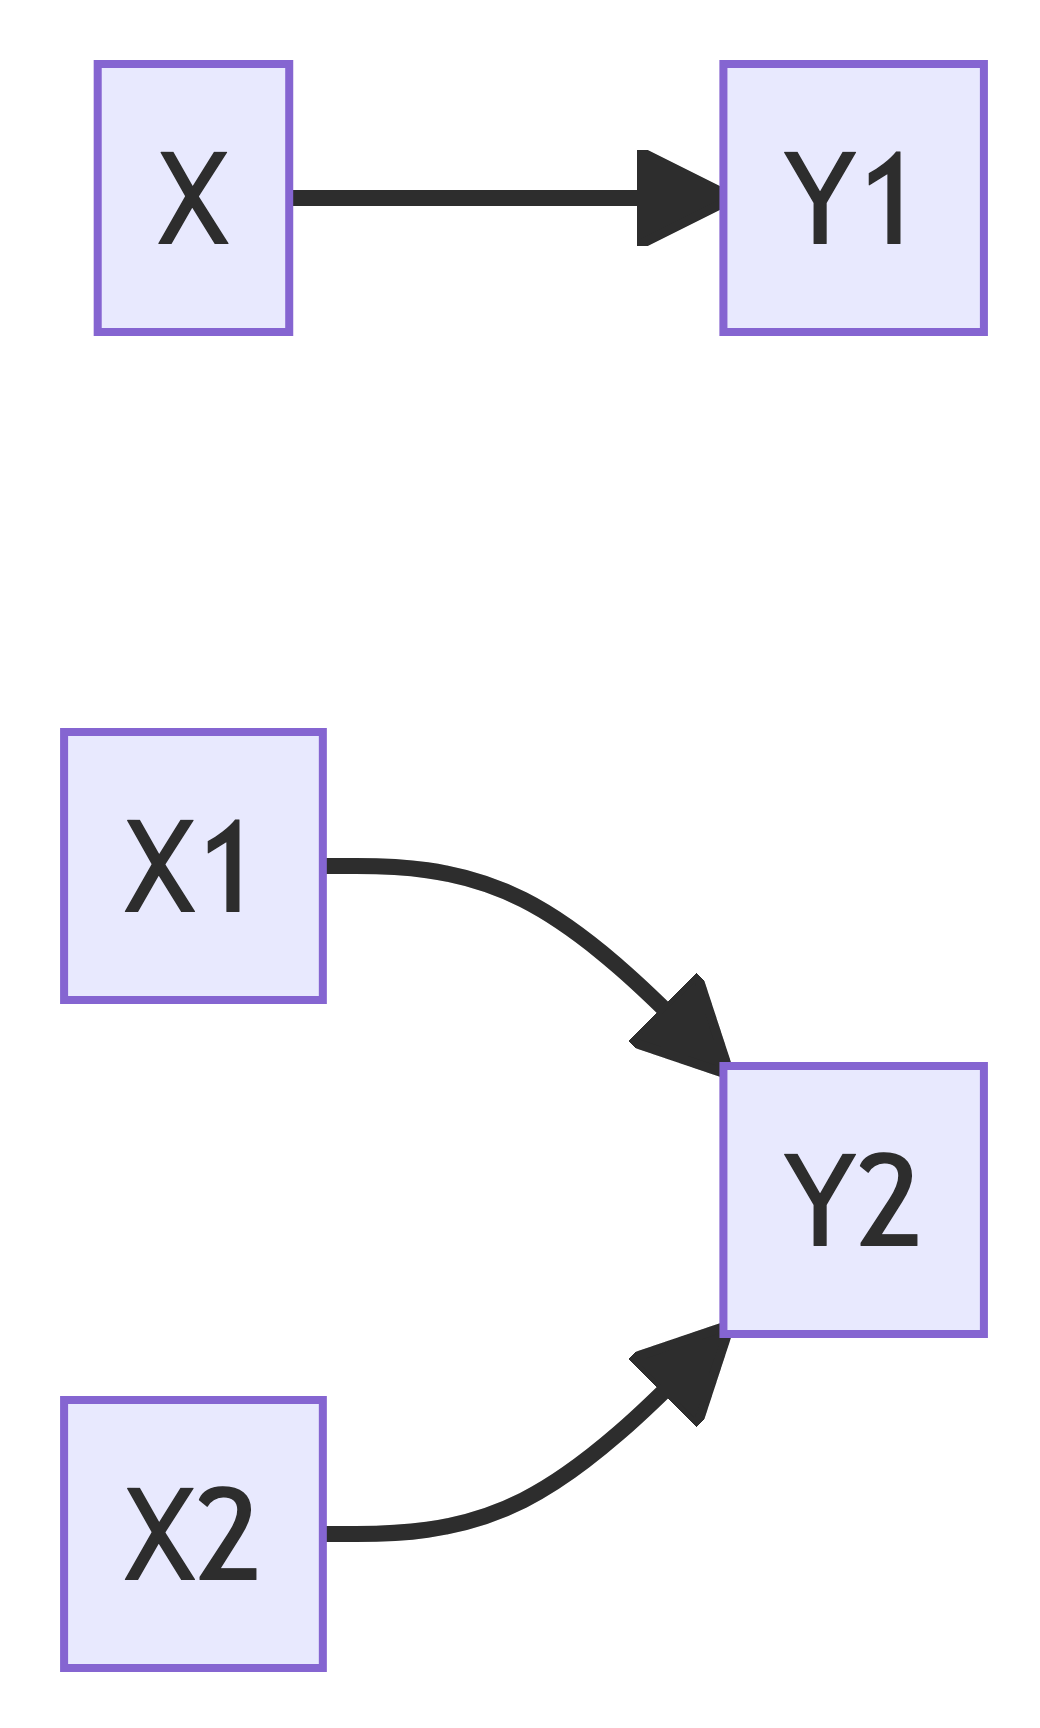
\includegraphics[width=6.5in,height=3.5in]{./regression2_files/figure-latex/mermaid-figure-1.png}

}

\end{figure}

}

\caption{\label{fig-multregr}One predictor (X) vs.~two predictors (X1,
X2)}

\end{figure}

given by Figure \textbf{?@fig-3dregr}, where a 3D account of a
regression is given. 3D means to input variables, and (which is always
the case) one output variable.

\begin{tcolorbox}[enhanced jigsaw, bottomrule=.15mm, toprule=.15mm, coltitle=black, breakable, title=\textcolor{quarto-callout-note-color}{\faInfo}\hspace{0.5em}{Note}, leftrule=.75mm, colback=white, bottomtitle=1mm, toptitle=1mm, left=2mm, opacityback=0, titlerule=0mm, colbacktitle=quarto-callout-note-color!10!white, opacitybacktitle=0.6, colframe=quarto-callout-note-color-frame, rightrule=.15mm, arc=.35mm]
Note that the slope in linear in both axis (X1 and X2).
\end{tcolorbox}

A different perspective is shown
\href{https://upload.wikimedia.org/wikipedia/commons/a/ae/2d_multiple_linear_regression.gif?20161014061355}{here},\\
where a 3D account of a regression is given. 3D means to input
variables, and (which is always the case) one output variable.

\begin{tcolorbox}[enhanced jigsaw, bottomrule=.15mm, toprule=.15mm, coltitle=black, breakable, title=\textcolor{quarto-callout-important-color}{\faExclamation}\hspace{0.5em}{Important}, leftrule=.75mm, colback=white, bottomtitle=1mm, toptitle=1mm, left=2mm, opacityback=0, titlerule=0mm, colbacktitle=quarto-callout-important-color!10!white, opacitybacktitle=0.6, colframe=quarto-callout-important-color-frame, rightrule=.15mm, arc=.35mm]
If the slope for one predictor is the same for all values of the other
predictor, then we say that no interaction is taking place.
\end{tcolorbox}

Here's a visualization of a 3D regression plane (not line) \emph{without
interaction}: constant slope in one axis, see the following figure,
\textbf{?@fig-3dregr2}.

\begin{figure}

{\centering 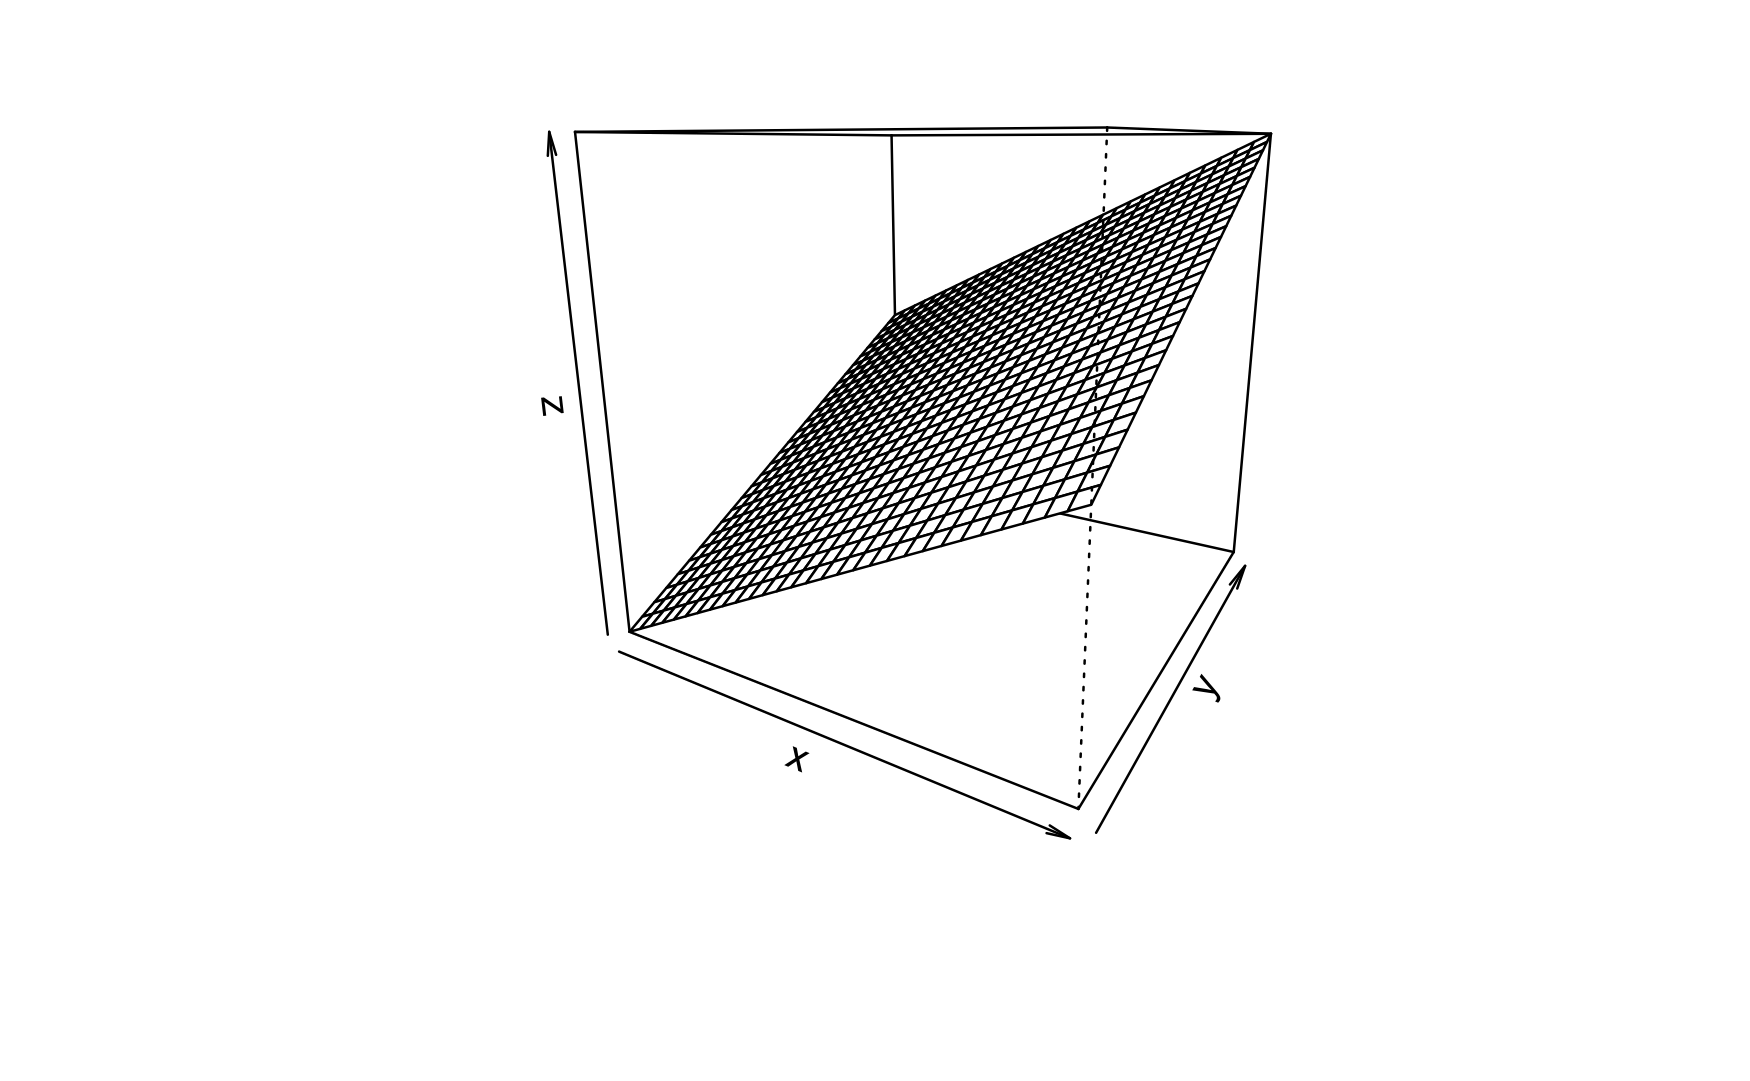
\includegraphics[width=5.83in,height=\textheight]{./img/3d1.png}

}

\caption{\label{fig-3dregr2-1}3D regression plane (not line) without
interaction}

\end{figure}

\begin{figure}

{\centering 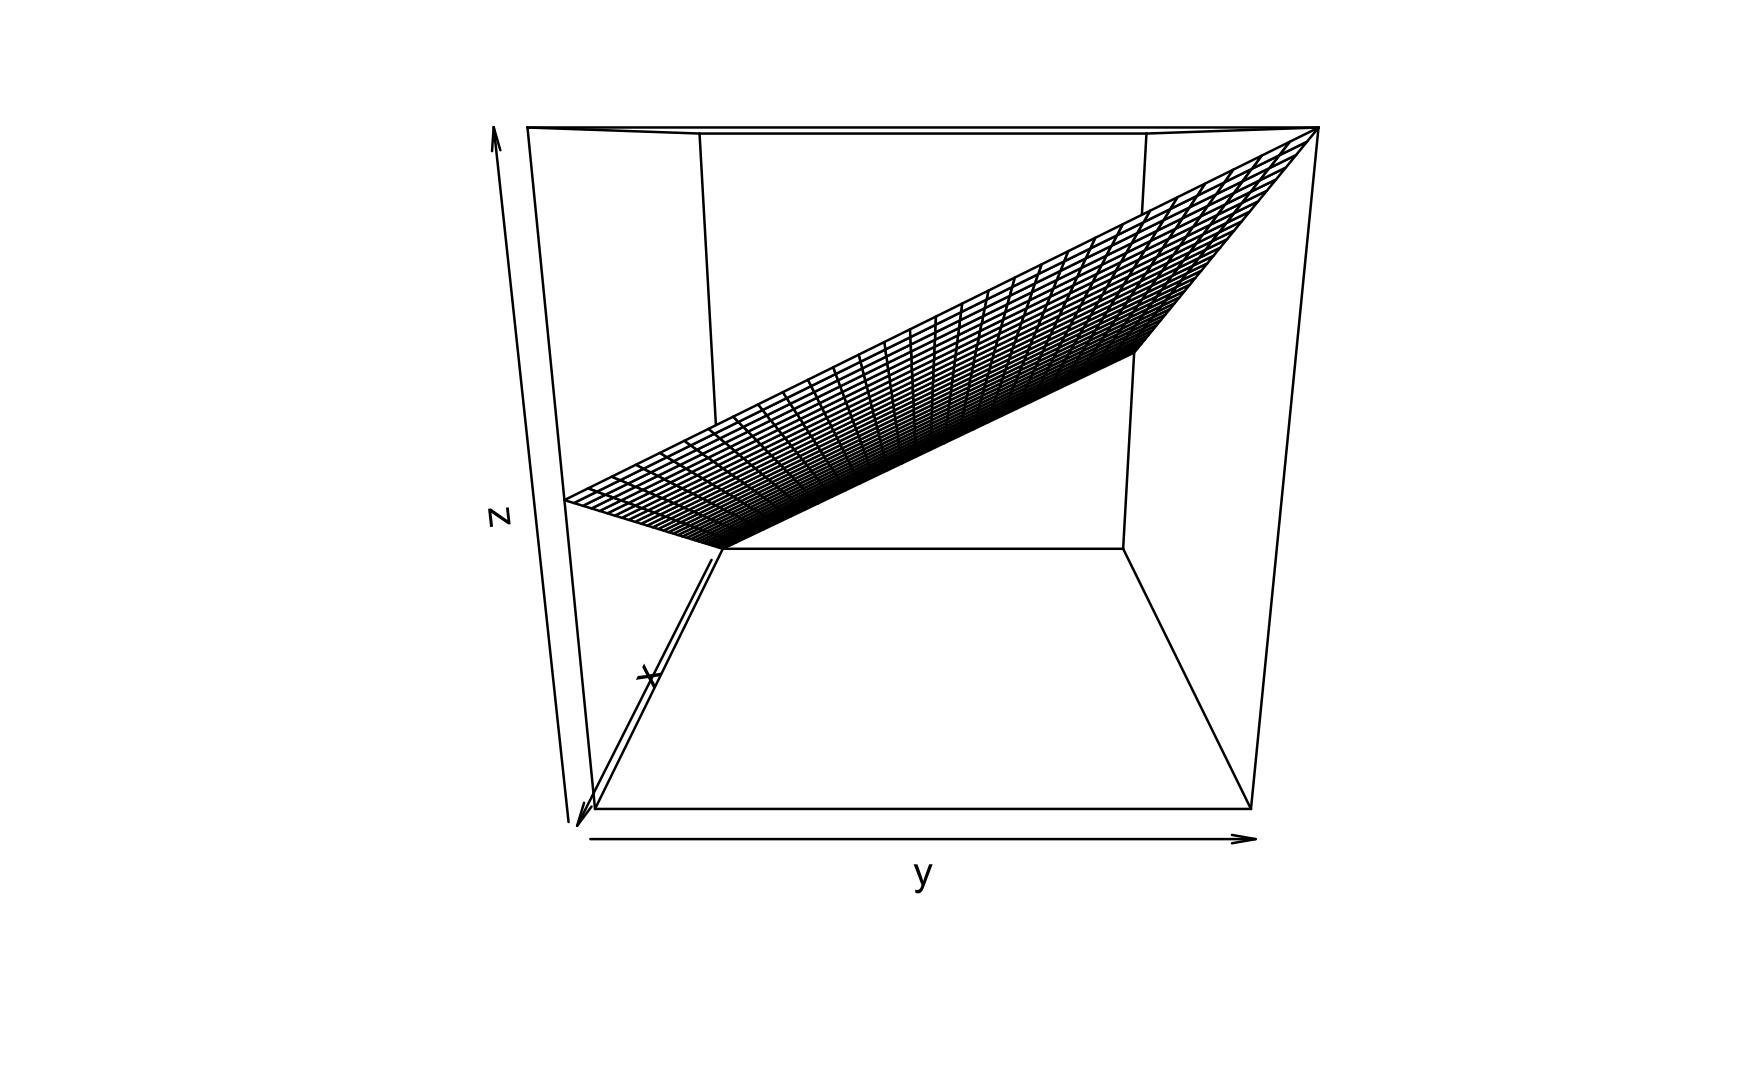
\includegraphics[width=5.83in,height=\textheight]{./img/3d2.png}

}

\caption{\label{fig-3dregr2-2}3D regression plane (not line) without
interaction}

\end{figure}

\begin{figure}

{\centering 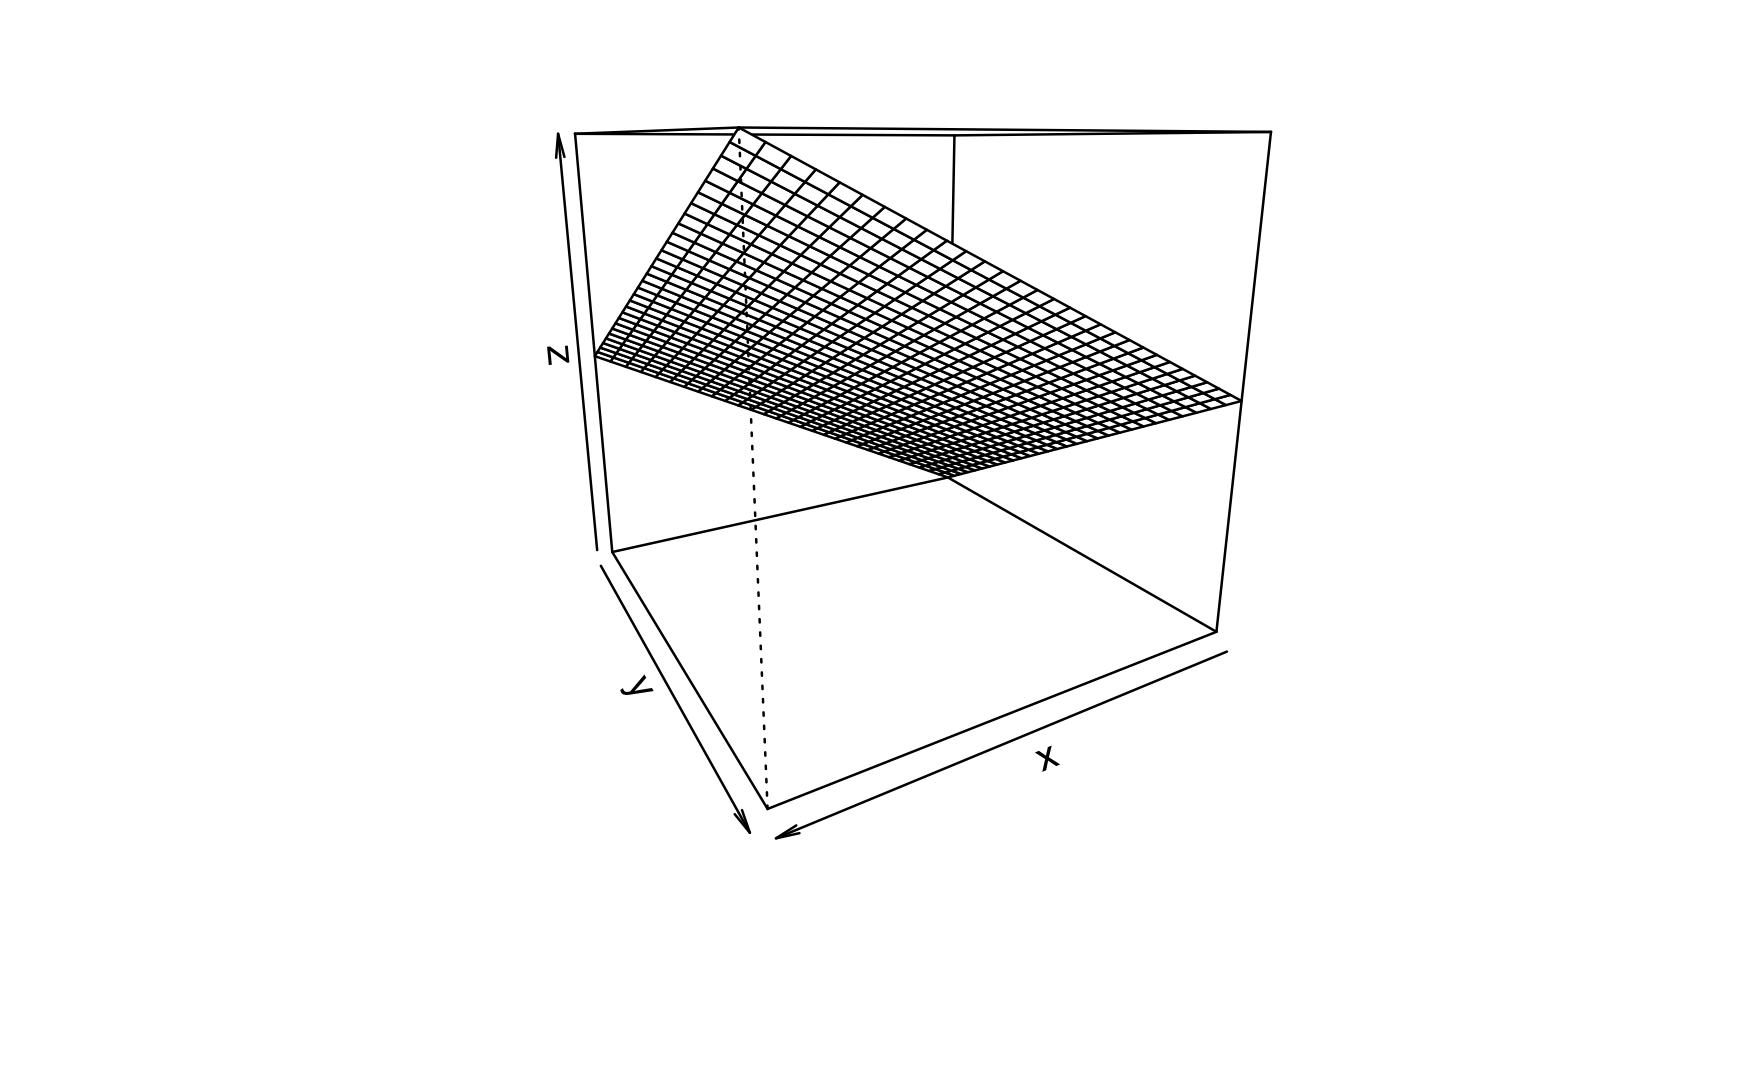
\includegraphics[width=5.83in,height=\textheight]{./img/3d3.png}

}

\caption{\label{fig-3dregr2-3}3D regression plane (not line) without
interaction}

\end{figure}

Note that in the above figure, the slope in each predictor axis equals
1, boringly. Hence the according 2D plots are boring, too.

For the sake of an example, consider this linear model:

\(mpg \sim hp + disp\)

Or, in more regression like terms:

\(y = \beta_0 + \beta_1 x_1 + \beta_2 x_2 + \epsilon\), where x1 is
\texttt{hp} and \texttt{x2} is \texttt{disp} in the \texttt{mtcars}
dataset.

In R terms:

\begin{Shaded}
\begin{Highlighting}[]
\NormalTok{lm3d }\OtherTok{\textless{}{-}} \FunctionTok{lm}\NormalTok{(mpg }\SpecialCharTok{\textasciitilde{}}\NormalTok{ hp }\SpecialCharTok{+}\NormalTok{ disp, }\AttributeTok{data =}\NormalTok{ mtcars)}
\end{Highlighting}
\end{Shaded}

The 3D plot is shown in Figure Figure~\ref{fig-mtcars3d}.

\begin{figure}

{\centering 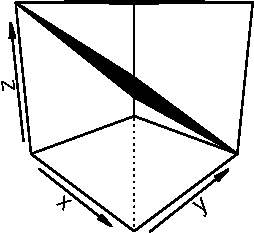
\includegraphics{./regression2_files/figure-pdf/fig-mtcars3d-1.pdf}

}

\caption{\label{fig-mtcars3d}mpg \textasciitilde{} hp + disp}

\end{figure}

Here are the two corresponding 2d (1 predictor) regression models:

\begin{Shaded}
\begin{Highlighting}[]
\NormalTok{lm1 }\OtherTok{\textless{}{-}} \FunctionTok{lm}\NormalTok{(mpg }\SpecialCharTok{\textasciitilde{}}\NormalTok{ hp, }\AttributeTok{data =}\NormalTok{ mtcars)}
\FunctionTok{plot}\NormalTok{(}\FunctionTok{estimate\_relation}\NormalTok{(lm1))}
\end{Highlighting}
\end{Shaded}

\begin{figure}[H]

{\centering 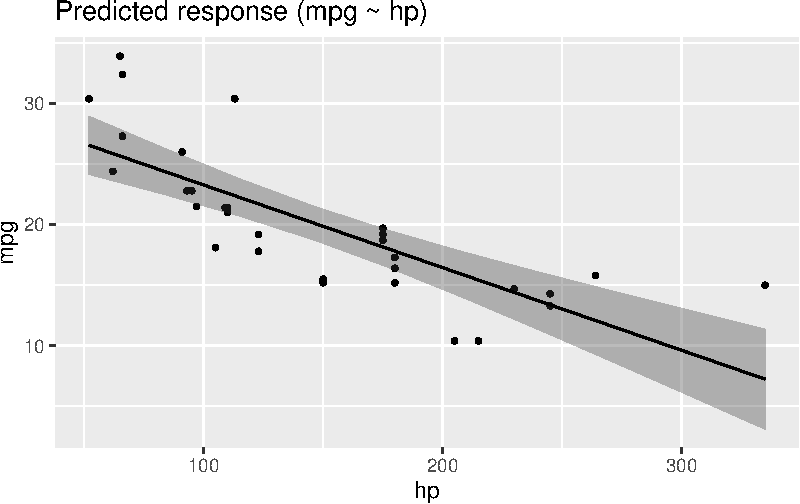
\includegraphics{./regression2_files/figure-pdf/unnamed-chunk-6-1.pdf}

}

\end{figure}

\begin{Shaded}
\begin{Highlighting}[]
\NormalTok{lm2 }\OtherTok{\textless{}{-}} \FunctionTok{lm}\NormalTok{(mpg }\SpecialCharTok{\textasciitilde{}}\NormalTok{ disp, }\AttributeTok{data =}\NormalTok{ mtcars)}
\FunctionTok{plot}\NormalTok{(}\FunctionTok{estimate\_relation}\NormalTok{(lm2))}
\end{Highlighting}
\end{Shaded}

\begin{figure}[H]

{\centering 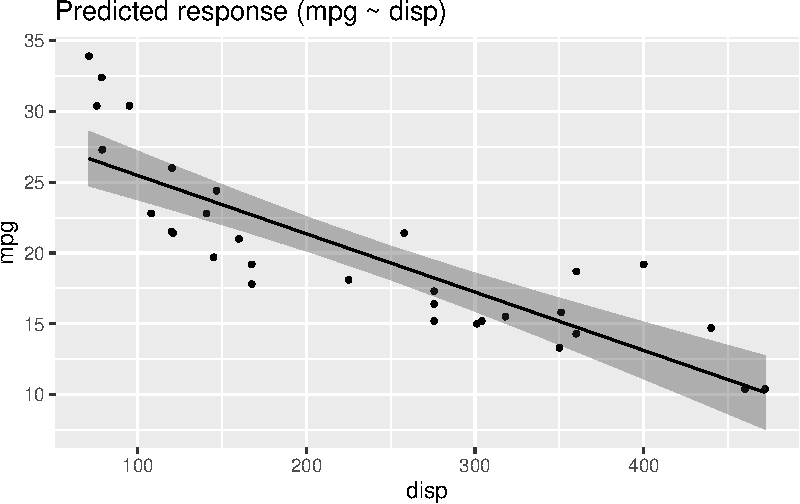
\includegraphics{./regression2_files/figure-pdf/unnamed-chunk-6-2.pdf}

}

\end{figure}

Checkout
\href{https://data-se.netlify.app/2022/04/19/3d-regression-plane-with-scatter-plot/}{this
post} for a visually slightly more appealing 3d regression plane.

\hypertarget{interaction-1}{%
\subsection{Interaction}\label{interaction-1}}

For interaction to happen we relax the assumption that the slope of
predictor 1 must be constant for all values of predictor 2.

In R, we specify an interaction model like this:

\begin{Shaded}
\begin{Highlighting}[]
\NormalTok{lm3d\_interact }\OtherTok{\textless{}{-}} \FunctionTok{lm}\NormalTok{(mpg }\SpecialCharTok{\textasciitilde{}}\NormalTok{ hp }\SpecialCharTok{+}\NormalTok{ disp }\SpecialCharTok{+}\NormalTok{ hp}\SpecialCharTok{:}\NormalTok{disp, }\AttributeTok{data =}\NormalTok{ mtcars)}
\end{Highlighting}
\end{Shaded}

The symbol \texttt{hp:disp} can be read as ``the interaction effect of
\texttt{hp} and \texttt{disp}''.

Here's a visual account, see Figure Figure~\ref{fig-mtcars3d-interact}.

\begin{figure}

{\centering 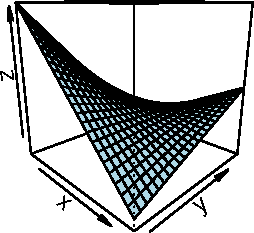
\includegraphics{./regression2_files/figure-pdf/fig-mtcars3d-interact-1.pdf}

}

\caption{\label{fig-mtcars3d-interact}mpg \textasciitilde{} hp + disp}

\end{figure}

Compare Figure~\ref{fig-mtcars3d-interact} and
Figure~\ref{fig-mtcars3d}.

In Figure~\ref{fig-mtcars3d-interact} you'll see that the lines along
the Y axis are not parallel anymore. Similarly, the lines along the X
axis are not parallel anymore.

\begin{tcolorbox}[enhanced jigsaw, bottomrule=.15mm, toprule=.15mm, coltitle=black, breakable, title=\textcolor{quarto-callout-important-color}{\faExclamation}\hspace{0.5em}{Important}, leftrule=.75mm, colback=white, bottomtitle=1mm, toptitle=1mm, left=2mm, opacityback=0, titlerule=0mm, colbacktitle=quarto-callout-important-color!10!white, opacitybacktitle=0.6, colframe=quarto-callout-important-color-frame, rightrule=.15mm, arc=.35mm]
If the regression lines (indicating different values of one predictor)
are \emph{not} parallel, we say that an interaction effect is taking
place.
\end{tcolorbox}

However, the \emph{difference} or \emph{change} between two adjacent
values (lines) is constant. This value is the size the regression
effect.

\hypertarget{interaction-made-simple}{%
\subsection{Interaction made simple}\label{interaction-made-simple}}

If you find that two sophisticated, consider the following simple case.

First, we mutate \texttt{am} to be a factor variable, in order to make
things simpler (without loss of generality).

\begin{Shaded}
\begin{Highlighting}[]
\NormalTok{mtcars2 }\OtherTok{\textless{}{-}}
\NormalTok{  mtcars }\SpecialCharTok{\%\textgreater{}\%} 
  \FunctionTok{mutate}\NormalTok{(}\AttributeTok{am\_f =} \FunctionTok{factor}\NormalTok{(am))}
\end{Highlighting}
\end{Shaded}

Now we use this new variable for a simple regression model:

\begin{Shaded}
\begin{Highlighting}[]
\NormalTok{lm\_interact\_simple }\OtherTok{\textless{}{-}} \FunctionTok{lm}\NormalTok{(mpg }\SpecialCharTok{\textasciitilde{}}\NormalTok{ disp }\SpecialCharTok{+}\NormalTok{ am\_f }\SpecialCharTok{+}\NormalTok{ disp}\SpecialCharTok{:}\NormalTok{am\_f, }\AttributeTok{data =}\NormalTok{ mtcars2)}
\end{Highlighting}
\end{Shaded}

Here's the plot, Figure Figure~\ref{fig-interact-simple}.

\begin{Shaded}
\begin{Highlighting}[]
\FunctionTok{plot}\NormalTok{(}\FunctionTok{estimate\_relation}\NormalTok{(lm\_interact\_simple))}
\end{Highlighting}
\end{Shaded}

\begin{figure}[H]

{\centering 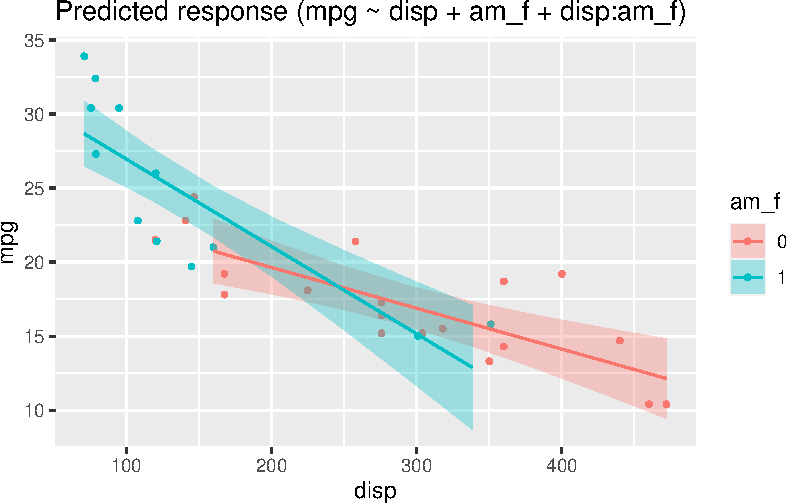
\includegraphics{./regression2_files/figure-pdf/fig-interact-simple-1.pdf}

}

\caption{\label{fig-interact-simple}A simple interaction model}

\end{figure}

In this picture, we see that the two regression lines are \emph{not}
parallel, and hence there is evidence of an interaction effect.

The interaction effect amounts to the \emph{difference} in slops in
Figure Figure~\ref{fig-interact-simple}.

One might be inclined to interpret Figure
Figure~\ref{fig-interact-simple} as an 3D image, where the one (reddish)
line is in the foreground and the blueish line in the background (or
vice versa, as you like). Given a 3D image (and hence 2 predictors), we
are where we started further above.

For completeness, here are the parameters of the model.

\begin{longtable}[]{@{}
  >{\raggedright\arraybackslash}p{(\columnwidth - 10\tabcolsep) * \real{0.2162}}
  >{\centering\arraybackslash}p{(\columnwidth - 10\tabcolsep) * \real{0.1757}}
  >{\centering\arraybackslash}p{(\columnwidth - 10\tabcolsep) * \real{0.1351}}
  >{\centering\arraybackslash}p{(\columnwidth - 10\tabcolsep) * \real{0.2703}}
  >{\centering\arraybackslash}p{(\columnwidth - 10\tabcolsep) * \real{0.0946}}
  >{\centering\arraybackslash}p{(\columnwidth - 10\tabcolsep) * \real{0.1081}}@{}}
\toprule()
\begin{minipage}[b]{\linewidth}\raggedright
Parameter
\end{minipage} & \begin{minipage}[b]{\linewidth}\centering
Coefficient
\end{minipage} & \begin{minipage}[b]{\linewidth}\centering
SE
\end{minipage} & \begin{minipage}[b]{\linewidth}\centering
95\% CI
\end{minipage} & \begin{minipage}[b]{\linewidth}\centering
t(28)
\end{minipage} & \begin{minipage}[b]{\linewidth}\centering
p
\end{minipage} \\
\midrule()
\endhead
(Intercept) & 25.16 & 1.93 & (21.21, 29.10) & 13.07 & \textless{}
.001 \\
disp & -0.03 & 6.22e-03 & (-0.04, -0.01) & -4.44 & \textless{} .001 \\
am f (1) & 7.71 & 2.50 & (2.58, 12.84) & 3.08 & 0.005 \\
disp * am f (1) & -0.03 & 0.01 & (-0.05, -7.99e-03) & -2.75 & 0.010 \\
\bottomrule()
\end{longtable}

\hypertarget{centering-variables}{%
\subsection{Centering variables}\label{centering-variables}}

The effect of of \texttt{am\_f} must be interpreted when \texttt{disp}
is zero, which does not make much sense.

Therefore it simplifies the interpretation of regression coefficients to
\emph{center} all input variables, by subtrating the mean value
(``demeaning'' or ``centering''):

\[x' = x - \bar{x}\] In R, this can be achieved e.g,. in this way:

\begin{Shaded}
\begin{Highlighting}[]
\NormalTok{mtcars3 }\OtherTok{\textless{}{-}} 
\NormalTok{mtcars2 }\SpecialCharTok{\%\textgreater{}\%} 
  \FunctionTok{mutate}\NormalTok{(}\AttributeTok{disp\_c =}\NormalTok{ disp }\SpecialCharTok{{-}} \FunctionTok{mean}\NormalTok{(disp))}
\end{Highlighting}
\end{Shaded}

\begin{Shaded}
\begin{Highlighting}[]
\NormalTok{lm\_interact\_simple2 }\OtherTok{\textless{}{-}} \FunctionTok{lm}\NormalTok{(mpg }\SpecialCharTok{\textasciitilde{}}\NormalTok{ disp\_c }\SpecialCharTok{+}\NormalTok{ am\_f }\SpecialCharTok{+}\NormalTok{ disp\_c}\SpecialCharTok{:}\NormalTok{am\_f, }\AttributeTok{data =}\NormalTok{ mtcars3)}
\FunctionTok{parameters}\NormalTok{(lm\_interact\_simple2)}
\end{Highlighting}
\end{Shaded}

\begin{verbatim}
Parameter         | Coefficient |       SE |         95% CI | t(28) |      p
----------------------------------------------------------------------------
(Intercept)       |       18.79 |     0.76 | [17.23, 20.36] | 24.63 | < .001
disp c            |       -0.03 | 6.22e-03 | [-0.04, -0.01] | -4.44 | < .001
am f [1]          |        0.45 |     1.39 | [-2.40,  3.30] |  0.32 | 0.748 
disp c * am f [1] |       -0.03 |     0.01 | [-0.05, -0.01] | -2.75 | 0.010 
\end{verbatim}

\hypertarget{predictor-relevance}{%
\section{Predictor relevance}\label{predictor-relevance}}

Given a model, we might want to know which predictor has the strongest
association with the outcome?

In order to answer this question, all predictor must have the same
scale. Otherwise the importance of a predictor would increase by 1000,
if we multiply each of the observations' values by the same factor.
However, this multiplication should not change the relevance of a
predictor.

A simple solution is to standardize all predictors to the same scale
(sd=1).

\begin{Shaded}
\begin{Highlighting}[]
\NormalTok{mtcars4 }\OtherTok{\textless{}{-}}
\NormalTok{  mtcars }\SpecialCharTok{\%\textgreater{}\%} 
  \FunctionTok{standardize}\NormalTok{(}\AttributeTok{select =} \FunctionTok{c}\NormalTok{(}\StringTok{"disp"}\NormalTok{, }\StringTok{"hp"}\NormalTok{, }\StringTok{"cyl"}\NormalTok{))}
\end{Highlighting}
\end{Shaded}

By the way, ``standardizing'' centers the variable by default to a mean
value of zero (by demeaning).

See:

\begin{Shaded}
\begin{Highlighting}[]
\FunctionTok{head}\NormalTok{(mtcars4}\SpecialCharTok{$}\NormalTok{disp)}
\end{Highlighting}
\end{Shaded}

\begin{verbatim}
[1] -0.57061982 -0.57061982 -0.99018209  0.22009369  1.04308123 -0.04616698
\end{verbatim}

\begin{Shaded}
\begin{Highlighting}[]
\FunctionTok{head}\NormalTok{(mtcars}\SpecialCharTok{$}\NormalTok{disp)}
\end{Highlighting}
\end{Shaded}

\begin{verbatim}
[1] 160 160 108 258 360 225
\end{verbatim}

Here's the SD:

\begin{Shaded}
\begin{Highlighting}[]
\FunctionTok{sd}\NormalTok{(mtcars4}\SpecialCharTok{$}\NormalTok{disp)}
\end{Highlighting}
\end{Shaded}

\begin{verbatim}
[1] 1
\end{verbatim}

\begin{Shaded}
\begin{Highlighting}[]
\FunctionTok{sd}\NormalTok{(mtcars}\SpecialCharTok{$}\NormalTok{disp)}
\end{Highlighting}
\end{Shaded}

\begin{verbatim}
[1] 123.9387
\end{verbatim}

And here's the mean value:

\begin{Shaded}
\begin{Highlighting}[]
\FunctionTok{mean}\NormalTok{(mtcars4}\SpecialCharTok{$}\NormalTok{disp)}
\end{Highlighting}
\end{Shaded}

\begin{verbatim}
[1] -9.084937e-17
\end{verbatim}

\begin{Shaded}
\begin{Highlighting}[]
\FunctionTok{mean}\NormalTok{(mtcars}\SpecialCharTok{$}\NormalTok{disp)}
\end{Highlighting}
\end{Shaded}

\begin{verbatim}
[1] 230.7219
\end{verbatim}

Now we are in a position to decide which predictor is more important:

\begin{Shaded}
\begin{Highlighting}[]
\NormalTok{m }\OtherTok{\textless{}{-}} \FunctionTok{lm}\NormalTok{(mpg }\SpecialCharTok{\textasciitilde{}}\NormalTok{ disp }\SpecialCharTok{+}\NormalTok{ hp }\SpecialCharTok{+}\NormalTok{ cyl, }\AttributeTok{data =}\NormalTok{ mtcars4)}
\FunctionTok{parameters}\NormalTok{(m)}
\end{Highlighting}
\end{Shaded}

\begin{verbatim}
Parameter   | Coefficient |   SE |         95% CI | t(28) |      p
------------------------------------------------------------------
(Intercept) |       20.09 | 0.54 | [18.98, 21.20] | 37.20 | < .001
disp        |       -2.33 | 1.29 | [-4.98,  0.31] | -1.81 | 0.081 
hp          |       -1.01 | 1.00 | [-3.06,  1.05] | -1.00 | 0.325 
cyl         |       -2.19 | 1.42 | [-5.11,  0.72] | -1.54 | 0.135 
\end{verbatim}

\hypertarget{exercises-1}{%
\section{Exercises}\label{exercises-1}}

\begin{itemize}
\tightlist
\item
  \href{https://datenwerk.netlify.app/posts/log-y-regr3/log-y-regr3/}{Predictor
  relevance}
\item
  \href{https://datenwerk.netlify.app/posts/adjustieren1/adjustieren1/}{Adjusting}
\item
  \href{https://datenwerk.netlify.app/posts/adjustieren2/adjustieren2/}{Adjusting
  2}
\item
  \href{https://datenwerk.netlify.app/posts/interpret-koeff/interpret-koeff/}{Interpreting
  Regression coefficients}
\end{itemize}

\hypertarget{lab-1}{%
\section{Lab}\label{lab-1}}

Get your own data, and build a simple model reflecting your research
hypothesis based on the topics covered in this chapter. If you are
lacking data (or hypothesis) get something close to it.

\hypertarget{glimpse-on-parameter-estimation}{%
\section{Glimpse on parameter
estimation}\label{glimpse-on-parameter-estimation}}

An elegant yet simple explanation of the math of parameter estimation
can be found
\href{https://godatadriven.com/blog/the-linear-algebra-behind-linear-regression/}{at
``go data driven''}. A similar approach is presented
\href{https://shainarace.github.io/LinearAlgebra/leastsquares.html}{here}.

Consider this geometric interpretation of the least square method in
Figure Figure~\ref{fig-leastsq}.

\begin{figure}

{\centering 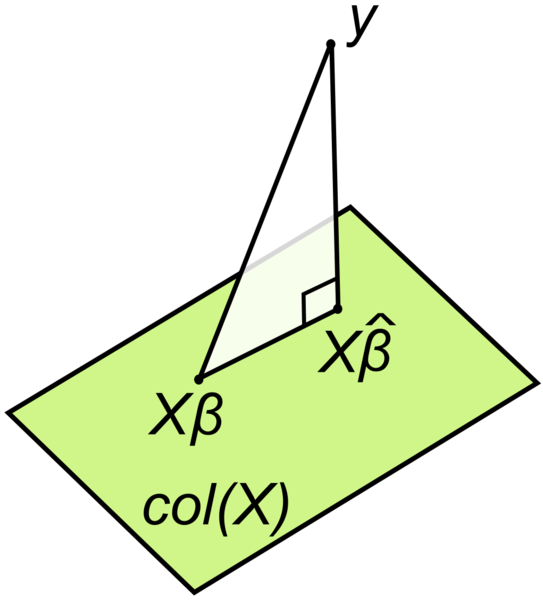
\includegraphics[width=0.25\textwidth,height=\textheight]{./img/543px-Linear_least_squares_geometric_interpretation.png}

}

\caption{\label{fig-leastsq}Geometric interpretation of the least square
method. Source: Oleg Alexandrov on Wikimedia}

\end{figure}

\hypertarget{literatur}{%
\section{Literatur}\label{literatur}}

A recent but already classic book on regression and inference (if this
is possible) is the book by Gelman, Hill, and Vehtari (2021). A great
textbook on statistical modelling (with a Bayesian flavor) was written
by McElreath (2020); it's suitable for PhD level.

Mathematical foundations can be found in Deisenroth, Faisal, and Ong
(2020).
\href{https://data-se.netlify.app/2022/06/13/free-resources-for-aspiring-data-adepts/}{Here's}
a collection of online resources tapping into statistics and machine
learning.

\bookmarksetup{startatroot}

\hypertarget{causality}{%
\chapter{Causality}\label{causality}}

\includegraphics[width=0.05\textwidth,height=\textheight]{./img/stern.png}

\hypertarget{r-packages-needed-for-this-chapter-3}{%
\section{R packages needed for this
chapter}\label{r-packages-needed-for-this-chapter-3}}

\begin{Shaded}
\begin{Highlighting}[]
\FunctionTok{library}\NormalTok{(tidyverse)}
\FunctionTok{library}\NormalTok{(ggdag)  }\CommentTok{\# optional  }
\end{Highlighting}
\end{Shaded}

\hypertarget{intro-to-causality}{%
\section{Intro to causality}\label{intro-to-causality}}

Check out this
\href{https://sebastiansauer-academic.netlify.app/uploads/Intro-to-Causality.pdf}{talk}.

\hypertarget{literature-3}{%
\section{Literature}\label{literature-3}}

Rohrer (2018) provides an accessible introduction to causal inference.
Slightly more advanced is the introduction by one of the leading figures
of the Field, Judea Pearl, Pearl, Glymour, and Jewell (2016). If your
after a text book on modelling that covers causal inference, and if you
like Bayesian statistics, than you should definitely check out McElreath
(2020).

\bookmarksetup{startatroot}

\hypertarget{case-studies}{%
\chapter{Case studies}\label{case-studies}}

\hypertarget{case-studies-on-explorative-data-analysis}{%
\section{Case studies on explorative data
analysis}\label{case-studies-on-explorative-data-analysis}}

\textbf{FALLSTUDIEN - NUR EXPLORATIVE DATENANALYSE}

\begin{itemize}
\item
  \href{https://allisonhorst.shinyapps.io/dplyr-learnr/\#section-welcome}{Datenjudo
  mit Pinguinen}
\item
  \href{https://data-se.netlify.app/2021/02/24/exercises-to-data-wrangling-with-the-tidyverse/}{Data-Wranglinng-Aufgaben
  zur Lebenserwartung}
\item
  \href{https://data-se.netlify.app/2021/02/24/case-study-data-vizualization-on-flight-delays-using-tidyverse-tools/}{Case
  study: data vizualization on flight delays using tidyverse tools}
\item
  \href{https://data-se.netlify.app/2020/12/07/ex-visualizing-diamonds/}{Aufgabe
  zur Datenvisualisierung des Diamantenpreises}
\item
  \href{https://data-se.netlify.app/2021/03/08/eda-zu-flugversp\%C3\%A4tungen/}{Fallstudie
  Flugverspätungen - EDA}
\item
  \href{https://data-se.netlify.app/2021/02/11/yacda-topgear/}{Fallstudie
  zur EDA: Top-Gear}
\item
  \href{https://data-se.netlify.app/2021/02/11/explorative-datenanalyse-zum-datensatz-oecd-wellbeing/}{Fallstudie
  zur EDA: OECD-Wellbeing-Studie}
\item
  \href{https://minimaxir.com/2018/07/imdb-data-analysis/}{Fallstudie
  zur EDA: Movie Rating}
\item
  \href{https://github.com/saghirb/WiP-tidyverse/blob/master/doc/WiP-tidyverse.pdf}{Fallstudie
  zur EDA: Women in Parliament}
\item
  \href{https://data-se.netlify.app/2021/05/27/datensatz-flights-finde-den-tag-mit-den-meisten-abfl\%C3\%BCgen/}{Finde
  den Tag mit den meisten Flugverspätungen, Datensatz `nycflights13'}
\item
  \href{http://varianceexplained.org/r/tidy-genomics/}{Cleaning and
  visualizing genomic data: a case study in tidy analysis}
\item
  \href{https://www.njtierney.com/post/2017/11/07/tidyverse-billboard/}{Tidyverse
  Case Study: Exploring the Billboard Charts}
\item
  \href{https://data-se.netlify.app/2021/11/27/analyse-der-rki-coronadaten/}{Analyse
  einiger RKI-Coronadaten: Eine reproduzierbare Fallstudie}
\item
  \href{https://www.opencasestudies.org/casestudies/ocs-healthexpenditure.html}{OpenCaseStudies
  - Health Expenditure}
\item
  \href{https://www.opencasestudies.org/ocs-bp-school-shootings-dashboard/\#Motivation}{Open
  Case Studies: School Shootings in the United States} - includes
  dashboards
\item
  \href{https://www.opencasestudies.org/ocs-bp-youth-disconnection/}{Open
  Case Studies: Disparities in Youth Disconnection}
\item
  \href{https://data-se.netlify.app/2021/05/28/yacsda-seitenspr\%C3\%BCnge/}{YACSDA
  Seitensprünge}
\item
  \href{https://www.opencasestudies.org/}{The Open Case Study Search}
  provides a nice collection of helpful case studies.
\item
  \href{https://fallstudien.netlify.app/}{ifes@FOM Fallstudienseite}
\end{itemize}

\hypertarget{case-studies-on-linear-modesl}{%
\section{Case studies on linear
modesl}\label{case-studies-on-linear-modesl}}

\textbf{FALLSTUDIEN - NUR LINEARE MODELLE}

\begin{itemize}
\item
  \href{https://youtu.be/5pBTHrnRIZY}{Beispiel für Prognosemodellierung
  1, grundlegender Anspruch, Video}
\item
  \href{https://data-se.netlify.app/2020/11/13/fallstudie-zur-regressionsanalyse-ggplot2movies/}{Beispiel
  für Ihre Prognosemodellierung 2, mittlerer Anspruch}
\item
  \href{https://data-se.netlify.app/2021/03/10/fallstudie-modellierung-von-flugversp\%C3\%A4tungen/}{Beispiel
  für Ihre Prognosemodellierung 3, hoher Anspruch}
\item
  \href{https://data-se.netlify.app/2021/03/10/fallstudie-modellierung-von-flugversp\%C3\%A4tungen/}{Fallstudie:
  Modellierung von Flugverspätungen}
\item
  \href{https://data-se.netlify.app/2021/02/24/modelling-movie-successes-linear-regression/}{Modelling
  movie successes: linear regression}
\item
  \href{https://data-se.netlify.app/2020/11/13/fallstudie-zur-regressionsanalyse-ggplot2movies/}{Movies}
\item
  \href{https://www.kaggle.com/code/ssauer/tmdb-simple-regression-beginners}{Fallstudie
  Einfache lineare Regression in Base-R, Anfängerniveau,
  Kaggle-Competition TMDB}
\item
  \href{https://data-se.netlify.app/2022/05/02/fallstudie-spritverbrauch/}{Fallstudie
  Sprit sparen}
\item
  \href{https://www.kaggle.com/code/saikatkumardey/linear-regression-case-study/notebook}{Fallstudie
  zum Beitrag verschiedener Werbeformate zum Umsatz}; eine Fallstudie in
  Python, aber mit etwas Erfahrung wird man den Code einfach in R
  umsetzen können (wenn man nicht in Python schreiben will)
\item
  \href{https://www.linkedin.com/pulse/practical-linear-regression-r-case-study-diamond-prices-valdeleon/?trk=public_profile_article_view}{Practical
  Linear Regression with R: A case study on diamond prices}
\item
  \href{https://stat-ata-asu.github.io/MultipleAndLogisticRegression/case-study-italian-restaurants-in-nyc.html}{Case
  Study: Italian restaurants in NYC}
\item
  \href{https://data-se.netlify.app/2021/05/19/vohrersgage-modellierung-des-preises-von-diamanten/}{Vorhersage-Modellierung
  des Preises von Diamanten}
\item
  \href{https://data-se.netlify.app/2021/05/25/modellierung-diamantenpreis-2/}{Modellierung
  Diamantenpreis 2}
\end{itemize}

\hypertarget{case-studies-on-machine-learning-using-tidymodels}{%
\section{Case studies on machine learning using
tidymodels}\label{case-studies-on-machine-learning-using-tidymodels}}

\textbf{FALLSTUDIEN - MASCHINELLES LERNEN MIT TIDYMODELS}

\begin{itemize}
\item
  \href{https://www.r-bloggers.com/2021/08/experimenting-with-machine-learning-in-r-with-tidymodels-and-the-kaggle-titanic-dataset/}{Experimenting
  with machine learning in R with tidymodels and the Kaggle titanic
  dataset}
\item
  \href{https://hansjoerg.me/2020/02/09/tidymodels-for-machine-learning/}{Tutorial
  on tidymodels for Machine Learning}
\item
  \href{https://www.kirenz.com/post/2021-02-17-r-classification-tidymodels/}{Classification
  with Tidymodels, Workflows and Recipes}
\item
  \href{https://www.kaggle.com/code/varimp/a-mostly-tidyverse-tour-of-the-titanic/report}{A
  (mostly!) tidyverse tour of the Titanic}
\item
  \href{https://www.kaggle.com/code/headsortails/personalised-medicine-eda-with-tidy-r/report}{Personalised
  Medicine - EDA with tidy R}
\item
  \href{https://www.kaggle.com/code/headsortails/tidy-titarnic/report}{Tidy
  TitaRnic}
\item
  \href{https://www.tidymodels.org/start/models/}{Fallstudie Seegurken}
\item
  \href{https://juliasilge.com/blog/student-debt/}{Sehr einfache
  Fallstudie zur Modellierung einer Regression mit tidymodels}
\item
  \href{https://www.gmudatamining.com/lesson-10-r-tutorial.html}{Fallstudie
  zur linearen Regression mit Tidymodels}
\item
  \href{https://github.com/sebastiansauer/covid-icu}{Analyse zum Verlauf
  von Covid-Fällen}
\item
  \href{https://onezero.blog/modelling-binary-logistic-regression-using-tidymodels-library-in-r-part-1/}{Fallstudie
  zur Modellierung einer logististischen Regression mit tidymodels}
\item
  \href{https://juliasilge.com/blog/multinomial-volcano-eruptions/}{Fallstudie
  zu Vulkanausbrüchen}
\item
  \href{https://juliasilge.com/blog/himalayan-climbing/}{Fallstudie
  Himalaya}
\item
  \href{https://juliasilge.com/blog/tuition-resampling/}{Fallstudien zu
  Studiengebühren}
\item
  \href{https://www.tidymodels.org/start/case-study/}{1. Modell der
  Fallstudie Hotel Bookings}
\item
  \href{https://github.com/sebastiansauer/datascience1/blob/main/Aufgaben/Thema8-Loesungen1.pdf}{Aufgaben
  zur logistischen Regression, PDF}
\item
  \href{https://bcullen.rbind.io/post/2020-06-02-tidymodels-decision-tree-learning-in-r/}{Fallstudie
  Oregon Schools}
\item
  \href{https://juliasilge.com/blog/wind-turbine/}{Fallstudie
  Windturbinen}
\item
  \href{https://www.gmudatamining.com/lesson-13-r-tutorial.html}{Fallstudie
  Churn}
\item
  \href{https://data-se.netlify.app/2020/12/14/titanic-tidymodels-boost/}{Einfache
  Durchführung eines Modellierung mit XGBoost}
\item
  \href{https://bcullen.rbind.io/post/2020-06-02-tidymodels-decision-tree-learning-in-r/}{Fallstudie
  Oregon Schools}
\item
  \href{https://www.gmudatamining.com/lesson-13-r-tutorial.html}{Fallstudie
  Churn}
\item
  \href{https://juliasilge.com/blog/ikea-prices/}{Fallstudie Ikea}
\item
  \href{https://juliasilge.com/blog/water-sources/}{Fallstudie
  Wasserquellen in Sierra Leone}
\item
  \href{https://dev.to/juliasilge/tuning-random-forest-hyperparameters-in-r-with-tidytuesday-trees-data-4ilh}{Fallstudie
  Bäume in San Francisco}
\item
  \href{https://juliasilge.com/blog/multinomial-volcano-eruptions/}{Fallstudie
  Vulkanausbrüche}
\item
  \href{https://juliasilge.com/blog/board-games/}{Fallstudie Brettspiele
  mit XGBoost}
\item
  \href{https://juliasilge.com/blog/lasso-the-office/}{Fallstudie Serie
  The Office}
\item
  \href{https://juliasilge.com/blog/nber-papers/}{Fallstudie NBER
  Papers}
\item
  \href{https://www.kaggle.com/ssauer/simple-linear-model-tidymodels}{Fallstudie
  Einfache lineare Regression mit Tidymodels, Kaggle-Competition TMDB}
\item
  \href{https://www.kaggle.com/code/ssauer/simple-rf-tuned}{Fallstudie
  Einfaches Random-Forest-Modell mit Tidymodels, Kaggle-Competition
  TMDB}
\item
  \href{https://www.kaggle.com/ssauer/tmdb-xgboost-tidymodels}{Fallstudie
  Workflow-Set mit Tidymodels, Kaggle-Competition TMDB}
\item
  \href{https://www.kaggle.com/code/modesty520/a-tutorial-with-tidymodels/report\#modeling}{Fallstudie
  Titanic mit Tidymodels bei Kaggle}
\item
  \href{https://www.kaggle.com/code/benthecoder/tidymodels-in-r-using-measles-data/notebook}{Einfache
  Fallstudie mit Tidymodels bei Kaggle}
\item
  \href{https://www.r-bloggers.com/2021/04/exploring-the-star-wars-prequel-renaissance-using-tidymodels-and-workflowsets/}{Exploring
  the Star Wars ``Prequel Renaissance'' Using tidymodels and
  workflowsets}
\end{itemize}

\bookmarksetup{startatroot}

\hypertarget{references}{%
\chapter*{References}\label{references}}
\addcontentsline{toc}{chapter}{References}

\hypertarget{refs}{}
\begin{CSLReferences}{1}{0}
\leavevmode\vadjust pre{\hypertarget{ref-deisenroth_mathematics_2020}{}}%
Deisenroth, Marc Peter, A. Aldo Faisal, and Cheng Soon Ong. 2020.
\emph{Mathematics for Machine Learning}. Cambridge ; New York, {NY}:
Cambridge University Press.

\leavevmode\vadjust pre{\hypertarget{ref-gelman_regression_2021}{}}%
Gelman, Andrew, Jennifer Hill, and Aki Vehtari. 2021. \emph{Regression
and Other Stories}. Analytical Methods for Social Research. Cambridge:
Cambridge University Press.

\leavevmode\vadjust pre{\hypertarget{ref-goodman_dirty_2008}{}}%
Goodman, Steven. 2008. {``A Dirty Dozen: Twelve p-Value
Misconceptions.''} \emph{Seminars in Hematology}, Interpretation of
quantitative research, 45 (3): 135--40.
\url{https://doi.org/10.1053/j.seminhematol.2008.04.003}.

\leavevmode\vadjust pre{\hypertarget{ref-hernan_second_2019}{}}%
Hernán, Miguel A., John Hsu, and Brian Healy. 2019. {``A Second Chance
to Get Causal Inference Right: A Classification of Data Science
Tasks.''} \emph{Chance} 32 (1): 42--49.
\url{https://doi.org/10.1080/09332480.2019.1579578}.

\leavevmode\vadjust pre{\hypertarget{ref-ismay_statistical_2020}{}}%
Ismay, Chester, and Albert Young-Sun Kim. 2020. \emph{Statistical
Inference via Data Science: A {ModernDive} into r and the Tidyverse}.
Chapman \& Hall/{CRC} the r Series. Boca Raton: {CRC} Press / Taylor \&
Francis Group. \url{https://moderndive.com/}.

\leavevmode\vadjust pre{\hypertarget{ref-mackay_scientific_2000}{}}%
MacKay, R. J., and R. W. Oldford. 2000. {``Scientific Method,
Statistical Method and the Speed of Light.''} \emph{Statistical Science}
15 (3): 254--78. \url{https://doi.org/10.1214/ss/1009212817}.

\leavevmode\vadjust pre{\hypertarget{ref-mcelreath_statistical_2020}{}}%
McElreath, Richard. 2020. \emph{Statistical Rethinking: A Bayesian
Course with Examples in r and Stan}. 2nd ed. {CRC} Texts in Statistical
Science. Boca Raton: Taylor; Francis, {CRC} Press.

\leavevmode\vadjust pre{\hypertarget{ref-pearl_causal_2016}{}}%
Pearl, Judea, Madelyn Glymour, and Nicholas P. Jewell. 2016.
\emph{Causal Inference in Statistics: A Primer}. Chichester, West
Sussex: Wiley.

\leavevmode\vadjust pre{\hypertarget{ref-poldrack_statistical_2022}{}}%
Poldrack, Russell. 2022. \emph{Statistical Thinking for the 21st
Century}.
\url{https://statsthinking21.github.io/statsthinking21-core-site/index.html}.

\leavevmode\vadjust pre{\hypertarget{ref-roback_beyond_2021}{}}%
Roback, Paul, and Julie Legler. 2021. \emph{Beyond Multiple Linear
Regression: Applied Generalized Linear Models and Multilevel Models in}.
1st ed. Chapman and Hall Texts in Statistical Science. Boca Raton: {CRC}
Press.

\leavevmode\vadjust pre{\hypertarget{ref-rohrer_thinking_2018}{}}%
Rohrer, Julia M. 2018. {``Thinking Clearly about Correlations and
Causation: Graphical Causal Models for Observational Data.''}
\emph{Advances in Methods and Practices in Psychological Science} 1 (1):
27--42. \url{https://doi.org/10.1177/2515245917745629}.

\leavevmode\vadjust pre{\hypertarget{ref-sauer_moderne_2019}{}}%
Sauer, Sebastian. 2019. \emph{Moderne Datenanalyse Mit r: Daten
Einlesen, Aufbereiten, Visualisieren Und Modellieren}. 1. Auflage 2019.
{FOM}-Edition. Wiesbaden: Springer.
\url{https://www.springer.com/de/book/9783658215866}.

\leavevmode\vadjust pre{\hypertarget{ref-wasserstein_asas_2016}{}}%
Wasserstein, Ronald L., and Nicole A. Lazar. 2016. {``The {ASA}'s
Statement on p-Values: Context, Process, and Purpose.''} \emph{The
American Statistician} 70 (2): 129--33.
\url{https://doi.org/10.1080/00031305.2016.1154108}.

\leavevmode\vadjust pre{\hypertarget{ref-wasserstein_moving_2019}{}}%
Wasserstein, Ronald L., Allen L. Schirm, and Nicole A. Lazar. 2019.
{``Moving to a World Beyond {` p{\textless{}}/i{\textgreater{}} p
{\textless{}} 0.05'}.''} \emph{The American Statistician} 73 (March):
1--19. \url{https://doi.org/10.1080/00031305.2019.1583913}.

\leavevmode\vadjust pre{\hypertarget{ref-r4ds}{}}%
Wickham, Hadley, and Garrett Grolemund. 2016. \emph{R for Data Science:
Visualize, Model, Transform, Tidy, and Import Data}. O'Reilly Media.
\url{https://r4ds.had.co.nz/index.html}.

\leavevmode\vadjust pre{\hypertarget{ref-wild_statistical_1999}{}}%
Wild, Chris J, and Maxine Pfannkuch. 1999. {``Statistical Thinking in
Empirical Enquiry.''} \emph{International Statistical Review} 67 (3):
223--48.

\end{CSLReferences}



\end{document}
